%% ****** Start of file apstemplate.tex ****** %
%%
%%
%%   This file is part of the APS files in the REVTeX 4.2 distribution.
%%   Version 4.2a of REVTeX, January, 2015
%%
%%
%%   Copyright (c) 2015 The American Physical Society.
%%
%%   See the REVTeX 4 README file for restrictions and more information.
%%
%
% This is a template for producing manuscripts for use with REVTEX 4.2
% Copy this file to another name and then work on that file.
% That way, you always have this original template file to use.
%
% Group addresses by affiliation; use superscriptaddress for long
% author lists, or if there are many overlapping affiliations.
% For Phys. Rev. appearance, change preprint to twocolumn.
% Choose pra, prb, prc, prd, pre, prl, prstab, prstper, or rmp for journal
%  Add 'draft' option to mark overfull boxes with black boxes
%  Add 'showkeys' option to make keywords appear
%\documentclass[aps,prl,preprint,groupedaddress]{revtex4-2}
\documentclass[prb,preprint,showpacs,preprintnumbers,amsmath,amssymb,longbibliography]{revtex4-1}

%\documentclass[aps,prl,preprint,superscriptaddress]{revtex4-2}
%\documentclass[aps,prl,reprint,groupedaddress]{revtex4-2}

% You should use BibTeX and apsrev.bst for references
% Choosing a journal automatically selects the correct APS
% BibTeX style file (bst file), so only uncomment the line
% below if necessary.
\bibliographystyle{apsrev4-2}

%\usepackage{showkeys}
\usepackage{todonotes}
\usepackage{graphicx}
%\usepackage{epstopdf,epsfig}
\usepackage{newtxtext}
\usepackage{newtxmath}
\usepackage{natbib}
\usepackage{hyperref}
\usepackage{mathtools}
\usepackage{commath}
\usepackage{tabularx}
\newtheorem{lemma}{Lemma}
\newtheorem{theorem}{Theorem}
\newtheorem{corollary}{Corollary}
\newcommand{\RomanNumeralCaps}[1]
\linenumbers


% Bryan's Marcros
\renewcommand{\aa}{\mathbf{a}}
\newcommand{\bd}{\partial}
\newcommand{\dd}{\mathbf{d}}
\newcommand{\DD}{\mathcal{D}}
\newcommand{\DDD}{\boldsymbol{\mathcal{D}}}
\newcommand{\SSS}{\mathcal{S}}
\newcommand{\eeta}{\boldsymbol{\eta}}
\newcommand{\FF}{\mathbf{F}}
\newcommand{\GG}{\mathbf{G}}
\newcommand{\JJ}{\mathbf{J}}
\newcommand{\nnu}{\boldsymbol{\nu}}
\newcommand{\ttau}{\boldsymbol{\tau}}
\newcommand{\ssigma}{\boldsymbol{\sigma}}
\newcommand{\rr}{\mathbf{r}}
\newcommand{\RR}{\mathbf{R}}
\renewcommand{\SS}{\mathbf{S}}
\newcommand{\ee}{\mathbf{e}}
\newcommand{\ff}{\mathbf{f}}
\newcommand{\xx}{\mathbf{x}}
\newcommand{\zz}{\mathbf{z}}
\newcommand{\XX}{\mathbf{X}}
\newcommand{\uu}{\mathbf{u}}
\renewcommand{\vv}{\mathbf{v}}
\newcommand{\yy}{\mathbf{y}}
\renewcommand{\tt}{\mathbf{t}}
\newcommand{\pderiv}[2]{\frac{\partial #1}{\partial #2}}
\newcommand{\jump}[1]{[\![ #1 ]\!]}


\begin{document}

% Use the \preprint command to place your local institutional report
% number in the upper righthand corner of the title page in preprint mode.
% Multiple \preprint commands are allowed.
% Use the 'preprintnumbers' class option to override journal defaults
% to display numbers if necessary
%\preprint{}

%Title of paper
\title{Collective behavior of Janus Particles  Suspended in a Viscous Fluid}

% repeat the \author .. \affiliation  etc. as needed
% \email \thanks, \homepage, \altaffiliation all apply to the current
% author. Explanatory text should go in the []'s, actual e-mail
% address or url should go in the {}'s for \email and \homepage.
% Please use the appropriate macro foreach each type of information

% \affiliation command applies to all authors since the last
% \affiliation command. The \affiliation command should follow the
% other information
% \affiliation can be followed by \email, \homepage, \thanks as well.
\author{Szu-Pei Fu$^{1}$, Rolf Ryham$^{2}$, Bryan Quaife$^{3}$ and Y.-N. Young$^{4}$}
%\email{peter.fu@trincoll.edu}
\affiliation{$^1$Department of Mathematics, Trinity College, Hartford, Connecticut 06106, USA\\
$^2$Department of Mathematics, Fordham University, Bronx, New York 10458, USA \\
$^3$Department of Scientific Computing, Florida State University, Tallahassee, Florida 32306, USA\\
$^4$Department of Mathematical Sciences, New Jersey Institute of Technology, Newark, New Jersey 07102, USA}

%\homepage[]{Your web page}
%\thanks{}
%\altaffiliation{}
%\author{Rolf Ryham}
%\email{rryham@fordham.edu}
%\affiliation{Department of Mathematics, Fordham University, Bronx, New York 10458, USA}
%
%\author{Bryan Quaife}
%\email{bquaife@fsu.edu}
 %\affiliation{Department of Scientific Computing, Florida State University, Tallahassee, Florida 32306, USA}
 %\author{Y.-N. Young}
 %\email{yyoung@njit.edu}
 %\affiliation{Department of Mathematical Sciences, New Jersey Institute of Technology, Newark, New Jersey 07102, USA}




%Collaboration name if desired (requires use of superscriptaddress
%option in \documentclass). \noaffiliation is required (may also be
%used with the \author command).
%\collaboration can be followed by \email, \homepage, \thanks as well.
%\collaboration{}
%\noaffiliation

\date{\today}

\begin{abstract}
%<<<<<<< HEAD
%Active colloidal systems with non-equilibrium self-organization is a long-standing challenge in biology. To understand how hydrodynamic flow may be used
%to actively control self-assembly of Janus particles (JPs),  we use a model recently developed for the many-body hydrodynamics of amphiphilic JPs suspended 
%in a viscous background flow (JFM, 941, 2022) to investigate how various bilayer structures arise from tuning the hydrophobicity/hydrophilicity of the JPs. 
%Focusing on three distributions of hydrophobicity we found JPs may assemble into uni-lamella, multi-lamella, and striated structures in a viscous fluid. 
%Under a linear flow and a Taylor-Green mixing flow,  we use three measures to quantify the collective dynamics of JP particles under a background flow: 
%(a) Free energy from the hydrophobic interactions between the JPs, (b) an order parameter for the ordering of JPs in terms of alignment of their directors, 
%and (c) a strain parameter that captures the deformation in the assembly. We found the dynamics of these three measures correlate well with the hydrodynamics 
%of JPs. These numerical provide insights into dynamic control of non-equilibrium active biological systems with similar self-organization.
% insert abstract here
%=======
  Active colloidal systems with non-equilibrium self-organization is a
  long-standing, challenging area in biology. To understand how
  hydrodynamic flow may be used to actively control self-assembly of
  Janus particles (JPs), we use a model recently developed for the
  many-body hydrodynamics of amphiphilic JPs suspended in a viscous
  background flow (JFM, 941, 2022). We investigate how various bilayer
  structures arise from tuning the hydrophobic properties of the
  JP-solvent interface. Focusing on a simple tuning of the
  hydrophobicity distribution, we found JPs assembled into uni-lamella,
  multi-lamella and striated structures. To introduce dynamics, we
  include a linear shear flow and a Taylor-Green mixing flow, and
  measure the collective dynamics of JP particles in terms of their (a)
  free energy from the hydrophobic interactions between the JPs, (b)
  order parameter for the ordering of JPs in terms of alignment of their
  directors, and (c) strain parameter that captures the deformation in
  the assembly. We characterized the effective material properties of
  the JP structures and found that the uni-lamellar structures increases
  orientation order under shear flow, the multilamellar structure
  behaves as a shear thinning fluid, and the striated structure
  possesses a finite yield stress. These numerical result provide
  insights into dynamic control of non-equilibrium active biological
  systems with similar self-organization.
%>>>>>>> 4f49b2ee420baba836cbb337c263b33981e1b096
\end{abstract}


%%%


% insert suggested keywords - APS authors don't need to do this
%\keywords{}

%\maketitle must follow title, authors, abstract, and keywords
\maketitle

% body of paper here - Use proper section commands
% References should be done using the \cite, \ref, and \label commands

\section{Introduction}
% Put \label in argument of \section for cross-referencing
%\section{\label{}}
Janus particles are colloids whose surfaces 
%have different properties. For example, it is common for the surface of a Janus
%particle to be 
are partly hydrophilic and hydrophobic (polar and non-polar).
More generally the surface of a Janus particle may have a spatial distribution of hydrophobicity/hydrophilicity.
In the absence of any imposed flow, Janus particles often self-assemble into
structures in a viscous solvent with tunable functions for biomedical engineering
applications~\cite{GheisariSahfieeAbbasiEtAl2021_DMR,
LiuYangHuangEtAl2016_Angew, LiWangYaoEtAl2019_Nanoscale, Bradley2016}.
Depending on the interactions between Janus particles (JPs) and the
surrounding viscous solvent, JPs self-assemble into oligomers of various
geometries and sizes~\cite{Bradley2017}. 


When driven by an external flow, 
dynamic rearrangement of JPs emerges naturally from the interactions between particles and fluid in colloidal
matter~\cite{Brandner2019,RevModPhys.93.025008}. Such colloidal hydrodynamics belongs to a wide class of
nonequilibrium self-organization in physics, often with complexity and features similar to that of 
biological systems such as living cells, bacterial baths, and
animal flocks~\cite{CollardGrosjeanVandewalle2020,Vutukuri2020}. A
long-standing challenge in fluid mechanics and material science is to
solve the ``inverse" problem of creating a model colloidal system that
will self-assemble into a prescribed
structure~\cite{PhysRevLett.128.256102}. For example, the framework of
geometrical frustration, which has been used to explain disordered
systems, could instead be used to design new, ordered systems, through
specific choices for the shapes or interactions of the
particles~\cite{Manoharan2015_Science}.

The many-body hydrodynamics of amphiphilic Janus particles assembled as
vesicles suspended in a viscous fluid in the inertialess regime (zero Reynolds number) has
been studied using boundary integral numerical
simulations~\cite{Fu20,Fu2022_JFM}. The dynamics of the JP suspension
results from the combination of long-range hydrodynamic interaction and
non-local interactions between JPs through the distribution of a
hydrophobic attraction potential (HAP).
%
In a quiescent flow, numerical simulations of a JP suspension showed
self-assembly into micelles and bilayers of JPs that provide an
alternative means for computing the mechanical moduli of a colloidal
membrane~\cite{NaTr00,Fu20,KrFiGuKaHa13}. Under background flows, the
hydrodynamics of a JP vesicle (a self-enclosed bilayer of JPs) exhibit
many familiar behaviors of a vesicle: elongation and
alignment along the extensional direction, tank-treading, and rupture of
a vesicle under shear flow~\cite{Fu2022_JFM}.

In this work, we take advantage of the flexibility of the HAP model to
examine the effects of varying hydrophobicity/hydrophilicity on JP surfaces.
Such variation of the boundary condition on JP surfaces may be realized in the experiments by using
chemicals to adjust the polarity of the viscous solvent, for example ({\bf references needed here}).
We show that a simple tuning of the hydrophobic distribution leads to transitions from unilamellar to
multilamellar or striated bilayer assembly (structures) of JPs. 
Focusing on the fluid-structure interactions that correspond to such transitions, 
we investigate the deformation of these
novel structures in background flows and map out their collective
behavior away from equilibrium.

%%%%%%%%%%%%%%%%%%%%%%%%%%%%%%%%%%%%%%%%%%%%%%%%%%%%%%%%%%%%%%%%%%%%%%%
\section{Governing Equations: Hydrophobic Attraction Potential Mobility Problem} 
The governing equations are a nonlinear system for the position and
orientation of a collection of rigid Janus particles. We first pose the
Stokes equations for the mobility problem giving the hydrodynamic
interactions for the particle suspension. The hydrophobic forces come
from solving a screened Laplace equation. Particle collisions are
avoided through a near-field, pair potential.

%%%%%%%%%%%%%%%%%%%%%%%%%%%%%%%%%%%%%%%%%%%%%%%%%%%%%%%%%%%%%%%%%%%%%%%
\subsection{Mobility problem}
%A suspension of $N_b$ Janus particles is immersed in a viscous solvent.
%RJR: In the above sentence, suspection and immersed are redundant 
The Janus particles are suspended in a viscous solvent. The particles
are disks of radius $c$, center $\aa_i$, and orientation $\theta_i$
relative to the horizontal axis, where $i = 1, \ldots, N_b$ and $N_b$ is
the number of particles. The domain $\Omega(t) \subset \mathbb{R}^2$ is
the solvent phase and $t$ is time. The boundary of $\Omega$ is
$\bd\Omega = \Gamma_1 \cup \cdots \cup \Gamma_{N_b}$, where $\Gamma_i$
is the boundary of Janus particle $i$. Assuming inertial terms are
negligible, we have 
\begin{alignat}{3}
\label{eq:stokes}
  -\mu \Delta \uu + \nabla p &= \mathbf{0}, && \xx \in \Omega, \\
\label{eq:stokesMass}
  \nabla\cdot \uu &= 0, \qquad && \xx \in \Omega, \\
\label{eq:stokesFarfield}
  \uu - \uu_\infty &\to \mathbf{0}, && |\xx| \to \infty,
\end{alignat}
where $\uu$ is the velocity of the solvent, $p$ is the pressure,
$\uu_\infty$ is the background flow velocity, and $\mu$ is the constant
viscosity. The solvent velocity satisfies the no-slip boundary condition
for a rigid body motion
\begin{align}
  \label{eq:rigid-vel}
  \uu(\xx) = \vv_i + \omega_i (\xx - \aa_i)^\perp, 
    \quad \xx \in \Gamma_i,
\end{align}
where $\vv_i$ is the translational velocity, $\omega_i$ is the angular
velocity, and $\langle x, y \rangle^{\perp} = \langle -y, x\rangle$. 

Without inertia, $(\uu, p)$ also satisfy the force-free and torque-free
conditions. This means that the force and torque from the hydrodynamic
stress on each particle balance the total force and torque coming from
the hydrophobic potential and repulsion. To compute this balance, we
define the free energy~\cite{Ma77, GoHaKo94, Fu20, Fu2022_JFM}
\begin{align}
\label{eq:free_energy}
F = \gamma
  \int_{\Omega} \left(\rho |\nabla u|^2 + \rho^{-1} u^2 \right)
\,d\xx
+ \frac{M}{2}
\sum_{j \neq i} 
P\left(\frac{|\aa_i - \aa_j|-2c}{\rho_0}\right),
\end{align}
where $u(\xx,t)$ is as an order parameter for the structure of water,
$\rho$ is a decay length, and $\gamma$ is an interfacial tension. 

The order parameter $u(\xx,t)$ is assumed to minimize the free energy
$F$. Its governing equations $u(\xx,t)$ are a screened Laplace equation
boundary value problem
\begin{gather}
  \label{eq:SL}
  -\rho^2 \Delta u + u = 0,\quad \xx \in \Omega, \\
  \label{eq:SLbc}
  u = g, \quad \xx \in \bd\Omega, \quad 
  u \rightarrow 0, \quad |\xx| \rightarrow \infty.
\end{gather}
The boundary condition $g$ encodes hydrophobic properties of the
particle-solvent interface.

The dimensionless repulsion profile $P$ takes the form $P(s) = 1 -
\sin(\pi s/2)$ for $0 \leq s < 1$ and $P(s) = 0$ for $1 \leq s <
\infty$. The parameter $\rho_0$ is an ``effective" repulsion distance between
particle surfaces, below which the steric repulsion between a pair of
JPs becomes important. The parameter $M$ is the repulsion modulus.

To calculate the force $\FF_i$ and torque $T_i$ on $\Gamma_i$ from the
free energy~\cite{Fu20}, we compute the variation of the domain of the
free energy~\eqref{eq:free_energy} subject
to~\eqref{eq:SL}--\eqref{eq:SLbc}, and obtain 
\begin{align}
  \label{eq:FandTdef}
  \FF_i = \int_{\Gamma_i} \mathbf{T}\nnu \, \dif s
  - \frac{M}{\rho_0}
  \sum_{j \neq i}
  \frac{\aa_i - \aa_j}{|\aa_i - \aa_j|}
P'\left(\frac{|\aa_i - \aa_j|-2c}{\rho_0}\right)
  ,\quad
T_i = \int_{\Gamma_i} (\xx - \aa_i)^{\perp}\cdot (\mathbf{T}\nnu) \, \dif s, 
\end{align}
for $i = 1,\ldots,N_b$ with particle outward normal $\nnu$.  The formulas
in \eqref{eq:FandTdef} involve the second-order hydrophobic stress tensor
\begin{align}
\mathbf{T} = \gamma \left[ \rho^{-1} u^2 \mathbf{I}
  + \rho \left(|\nabla u|^2 \mathbf{I} - 2\nabla u \nabla u^T\right)\right].
\end{align}
The repulsion is rotationally symmetric and
does not contribute to the torque $T_i$.

Since the force and torque from the hydrodynamic stress on each particle
balance the total force and torque coming from the hydrophobic potential
and repulsion, we have
\begin{equation}
  \label{eq:force}
 \int_{\Gamma_i} \ssigma \cdot \nnu \, \dif s = \FF_i, \quad
 \int_{\Gamma_i} (\xx - \aa_i)^\perp \cdot 
  (\ssigma \cdot \nnu) \, \dif s = T_i,
  \quad i=1,\ldots,N_b,
\end{equation}
where $\ssigma = -p \mathbf{I} + \mu \left(\nabla \uu + \nabla \uu^T
\right)$ is the hydrodynamic stress tensor.

To perform a single time step, we first solve for the HAP by
solving~\eqref{eq:SL}--\eqref{eq:SLbc}, and then compute the force and
torque~\eqref{eq:FandTdef}. Then the Stokes
equations~\eqref{eq:stokes}--\eqref{eq:stokesFarfield} are solved, and
the force-free and torque-free conditions are used to compute the rigid
body motion~\eqref{eq:rigid-vel}.
Once~\eqref{eq:stokes}--\eqref{eq:force} have been solved, the
velocities $(\vv_i, \omega_i)$ from~\eqref{eq:rigid-vel} update the
particle positions and orientations.


%%%%%%%%%%%%%%%%%%%%%%%%%%%%%%%%%%%%%%%%%%%%%%%%%%%%%%%%%%%%%%%%%%%%%%%
\subsection{Boundary integral representations}
We recast~\eqref{eq:stokes}--\eqref{eq:rigid-vel}
and~\eqref{eq:SL}--\eqref{eq:SLbc} as boundary integral equations (BIEs)
and discretize each BIE at $N$ points on each of the $N_b$ particles
with a collocation method. To express the solution of
\eqref{eq:SL}--\eqref{eq:SLbc}, we adopt the double layer potential
\begin{align}
\label{eq:SL_BIE}
u({\xx}) = \DD[\sigma](\xx) = \int_\Gamma 
  \pderiv{G(\xx-\yy)}{\nnu_\yy}\sigma(\yy)\, \dif s_\yy, 
  \quad \xx \in \Omega,
\end{align}
where $G(\xx) = \frac{1}{2\pi}K_0(|\xx|/\rho)$ is the fundamental
solution to the screened Laplace equation~\eqref{eq:SL}, $K_0$ is the
zeroth-order modified Bessel function of the first kind, $\nnu_\yy$ is
the unit outward normal at $\yy$, and $\sigma$ is a scalar-valued
density function. The subscript in $\dif s_\yy$ denotes integration with
respect to $\yy \in \Gamma$. To satisfy the boundary
condition~\eqref{eq:SLbc}, the density function must satisfy\cite{Hsiao2008}
\begin{align}
  \label{eq:SL_BIE2}
  g(\xx) = \frac{1}{2} \sigma(\xx) + \DD[\sigma](\xx), \quad
    \xx \in \Gamma.
\end{align}

For the velocity, we use the representation
\begin{align}
  \label{eq:velocity}
  \uu(\xx) = \uu_\infty(\xx) + \DDD[\eeta](\xx) + 
    \sum_{i=1}^{N_b} \left(\SS(\xx,\aa_i) \cdot \FF_i + 
    \RR(\xx,\aa_i) T_i\right), \quad \xx \in \Omega,
\end{align}
where $\eeta$ is a vector-valued density function and
\begin{align}
  \DDD[\eeta](\xx) = \frac{1}{\pi} \int_{\Gamma} 
    \frac{(\xx - \yy) \cdot \nnu_\yy}{|\xx - \yy|^2}
    \frac{(\xx - \yy) \otimes (\xx - \yy)}{|\xx - \yy|^2}
    \cdot \eeta(\yy)\, \dif s_\yy.
\end{align}
The Stokeslets and Rotlets are
\begin{align}
  \SS(\xx,\aa_i) = \frac{1}{4\pi} \left(-\log |\rr|\mathbf{I} +
    \frac{\rr \otimes \rr}{|\rr|^2}\right), \quad 
  \RR(\xx,\aa_i) = \frac{1}{4\pi} \frac{\rr^\perp}{|\rr|^2}, 
\end{align}
respectively, where $\rr = \xx - \aa_i$~\cite{pow-mir1987}. Letting
$\xx$ approach $\Gamma_i$ in~\eqref{eq:velocity}, applying the jump
condition of the double layer potential~\cite{poz1992}, and imposing the
no-slip boundary condition~\eqref{eq:rigid-vel}, the density function
$\eeta$, translational velocity $\vv_i$, and rotational velocity
$\omega_i$ satisfy
\begin{alignat}{3}
  \label{eq:vel_BLM_rep}
  \vv_i + \omega_i (\xx - \aa_i)^\perp &= \uu_\infty(\xx)
    -\frac{1}{2} \eeta(\xx) + \DDD[\eeta](\xx) 
    + \sum_{j=1}^{N_b} 
    \left(\SS(\xx,\aa_j) \cdot \FF_j + \RR(\xx,\aa_j) T_j\right),\\
  \label{eq:vel_BLM_rep2}
  \int_{\Gamma_i} \eeta \, \dif s &= \mathbf{F}_i, \quad
  \int_{\Gamma_i} \eeta \cdot (\xx-\aa_i)^\perp \, \dif s = T_i,
\end{alignat}
for $\xx \in \Gamma_i$ and $i = 1,\ldots,N_b$.
Equation~\eqref{eq:vel_BLM_rep}--\eqref{eq:vel_BLM_rep2} does have a
unique solution, but we note that alternative full-rank layer potential
representations for rigid body motions are possible~\cite{rac-gre2016,
cor-gre-rac-vee2017}.

We discretize~\eqref{eq:SL_BIE2}
and~\eqref{eq:vel_BLM_rep}--\eqref{eq:vel_BLM_rep2} using high-order
interpolation-based quadrature rules. Integrals that are smooth are
computed with the spectrally-accurate trapezoid rule, and
nearly-singular integrals, caused by close contact between two
particles, are computed with a high-order interpolation-based quadrature
rule~\cite{qua-bir2014}.

After discretizing and applying quadrature, the result is an $NN_b
\times NN_b$ and $2NN_b \times 2NN_b$ linear system
for~\eqref{eq:SL_BIE2}
and~\eqref{eq:vel_BLM_rep}--\eqref{eq:vel_BLM_rep2}, respectively.
These are solved with matrix-free GMRES, and we guarantee that the
number of GMRES iterations is mesh-independent by using second-kind
BIEs. Once the translational and rotational velocity are computed, the
position and orientation of each JP is updated using the second-order
Adams-Bashforth scheme.

%Once the translational and angular velocities $\vv_i, \omega_i$
%have been determined, a second-order Adams-Bashforth scheme updates the particle
%positions and orientations:
%\begin{equation}
%  \label{eq:adams-bashforth}
%  \begin{aligned}
%    \aa_i(t_{n+2}) &=
%\aa_i(t_{n+1})
%+ \tfrac{3}{2}\Delta t \vv_i(t_{n+1})
%- \tfrac{1}{2}\Delta t \vv_i(t_{n}),\\
%    \theta_i(t_{n+2}) &=
%\theta_i(t_{n+1})
%+ \tfrac{3}{2}\Delta t \omega_i(t_{n+1})
%- \tfrac{1}{2}\Delta t \omega_i(t_{n}).
% \end{aligned}
%\end{equation}


\section{Model parameters and boundary conditions}
The interactions generated by the HAP-mobility problem formulation
\eqref{eq:stokes}--\eqref{eq:force}
lead to particle self-assembly for a broad range of parameters and
boundary conditions.  Generally speaking, the effective distance of the
hydrophobic interaction is set by the screening length $\rho$.
Smaller values of the repulsion distance $\rho_0$ decrease the distance
where attraction and repulsion are in balance and lead to more compact
particle assemblies. 
The rate of self assembly is proportional to the interfacial tension $\gamma$,
and inversely proportional to solvent viscosity $\mu$; it is
roughly inversely proportional to screening length $\rho.$

To give our system physical units, we set the model parameters
using phospholipids as a characteristic amphiphile in water \cite{Boal}.
For solvent viscosity, we use $\mu = 1$ mPa s for the viscosity
of water at room temperature.
Pure lipid components give a range
of interfacial tensions $0.7$ -- $5.3$ pN nm$^{-1}$
~\cite{KUZMIN2005, Petelska2012,Jackson2016,GarciaSaez}.
As in our previous works\cite{Fu20,Fu2022_JFM},
we use $\gamma=4.1$ pN nm$^{-1}$ since this value gave
good agreement with elastic moduli of lipid bilayers.
The particle radius $c = 1.25$ nm
gives a diameter representative of phospholipid length \cite{Boal},
and the screening length $\rho = 5$ nm
derives from experimental force-distance measurements of hydrophobic
attraction \cite{ErLjCl89,Lietal05,Israelachvili80,Jackson2016}.
Based on empirical studies, the repulsion modulus $M = 2$ pN
and repulsion distance $\rho_0 = 0.5$ nm give an interparticle
distance around one particle radius.  This 
ensures the accuracy of the boundary integral representations
\eqref{eq:SL_BIE} and \eqref{eq:velocity}
without having to employ overly aggresive mesh refinement. 
Altogether, the above parameter set gives
a characteristic time $1$
ns and characteristic length $1$ nm.

\begin{figure}[h!]
\begin{center}
  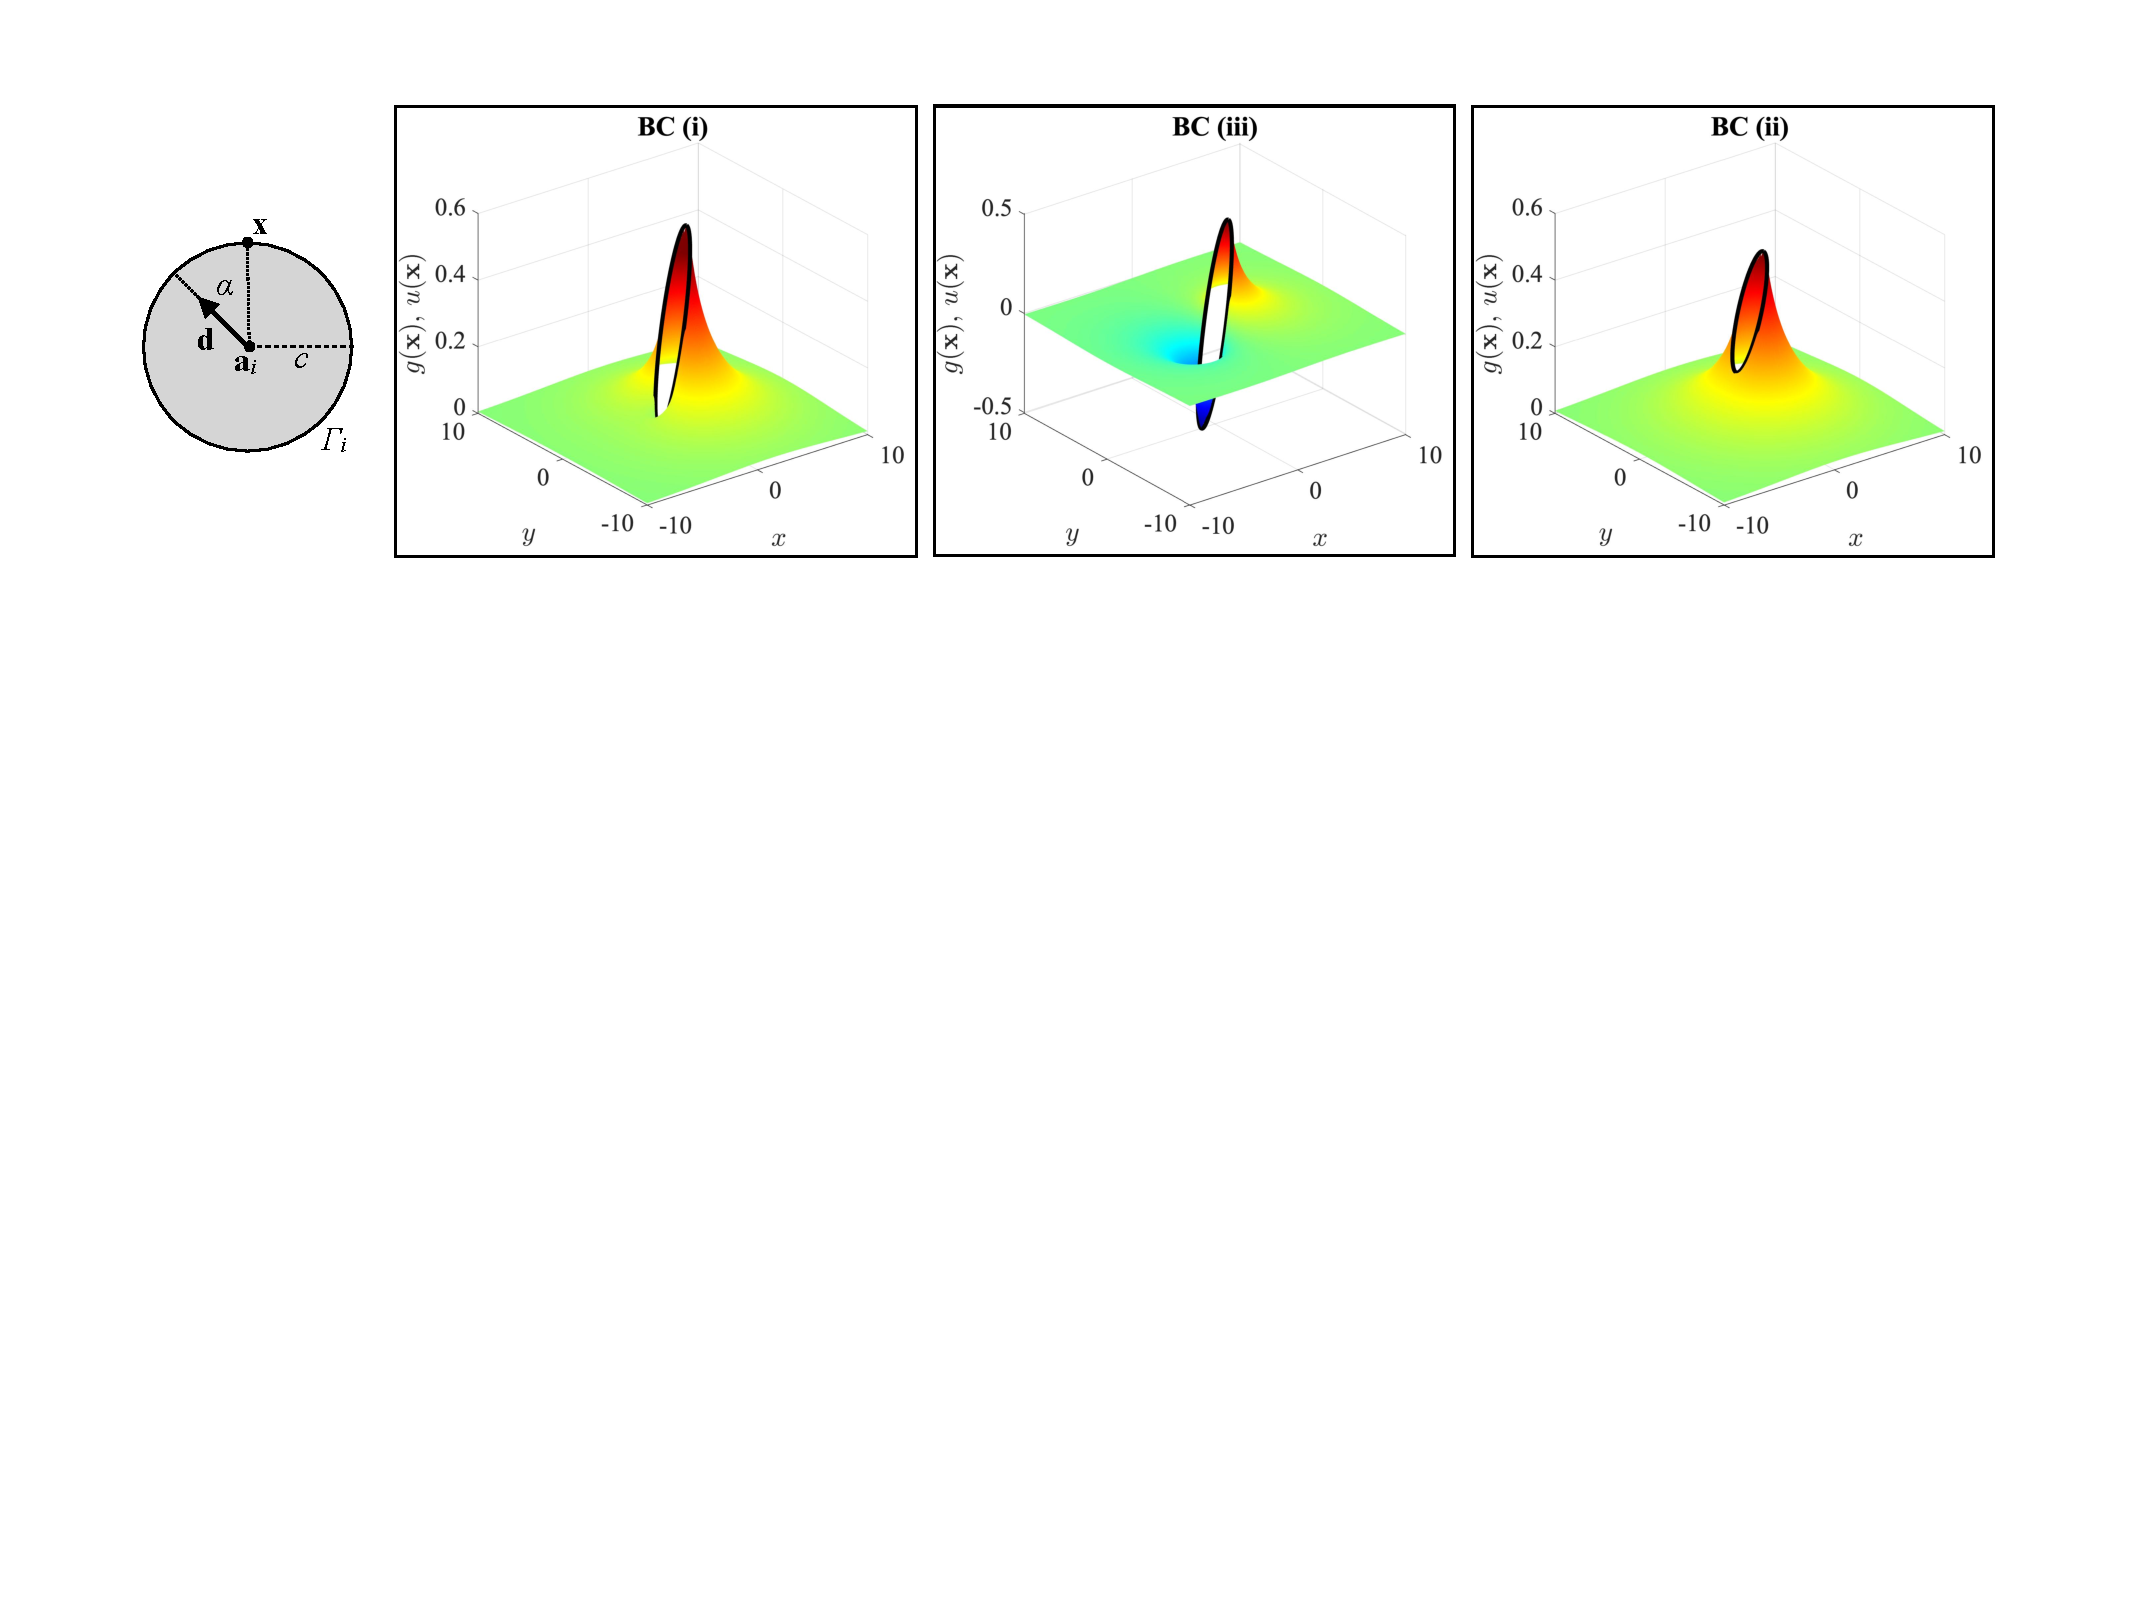
\includegraphics[width=\textwidth]{Figures/Figure0.pdf}
\end{center}
\begin{caption}{\label{fig:boundary_conditions}
    The leftmost diagram illustrates the particle
    $\Gamma_i$ with center $\aa_i$, radius $c$, and director $\dd$,
    along with the angle $\alpha$ used to define $g(\xx)$ in \eqref{eq:bc-type}.
    The three righ plots show $g(\xx)$ (black curve) for BC (i), (ii), and (iii)
    when $\dd = (1,0)$. The surfaces are the respective solutions
    $u(\xx)$ of \eqref{eq:SL} for a single, isolated particle.  
  }
\end{caption}
\end{figure}


\subsection{Boundary conditions and equilibrium configurations}
The boundary condition $g(\xx)$ in
\eqref{eq:SLbc} defines the spatial distribution of
hydrophobicity and hydrophilicity.  On a hydrophobic region of the
particle surface, representing a hydrocarbon-water interface,
for example, $g(\xx)$ takes relatively large values.
On an apolar, hydrophilic region, $g(\xx)$ is close to zero.

In the present work, we consider boundary conditions of the form
\begin{align}
  \label{eq:bc-type}
g(\xx) = a(b + \cos \alpha),\quad a = (\pi c(2b^2 + 1))^{-1/2},\quad \xx \in \Gamma_i,
\end{align}
where $\alpha$ is the angle between the vector $\xx - \aa_i$ and 
the particle director $\dd_i = (\cos \theta_i, \sin \theta_i)$.
The parameter $a$ normalizes the boundary conditions 
so that $\int_{\Gamma_i} g^2(\xx) \, \dif s =  1$.
The motivation for this normalization is that the hydrophobic attraction
part of the free energy converges to the integral of the square of the boundary
data in the zero-screening length limit.  
We refer to the side of the particle where $\alpha = 0$
as the tail and the side where $\alpha = \pi$ as the head. 


We set $\max g>0$ to guarantee at least partial hydrophobicity of the JP
surface.  Then, the boundary condition (BC) can be classified into three
categories: $\min g(\xx) = 0$, $\min g(\xx) >0$, and $\min g(\xx) <0$
where the extrema are taken for $\xx \in \Gamma_i$.  These three
categories correspond to three characteristic values of $b$ in
\eqref{eq:bc-type}: $b=1$, $b=2$ and $b=0$, respectively. 
%
To see the effect of the shift parameter $b$, we simulate the dynamics
of 198 particles and 60 particles in a quiescent flow as shown in
Figure~\ref{fig:relax}. Three distinct configurations emerge: (i)
bilayer for $b = 1$, (ii) multilamellar for $b = 2$, and (iii) striated
for $b = 0$.


\begin{figure}[h!]
\begin{center}
  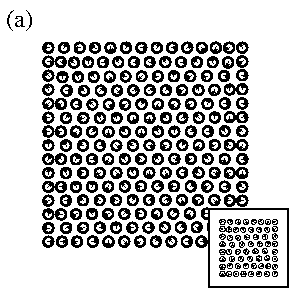
\includegraphics[height=0.3\textheight]{Nb198a_inset.pdf}
  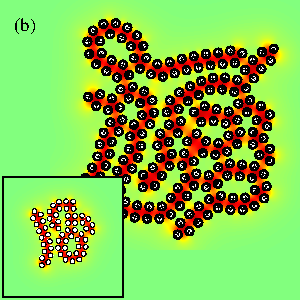
\includegraphics[height=0.3\textheight]{Nb198b_eta_inset.pdf}\\
  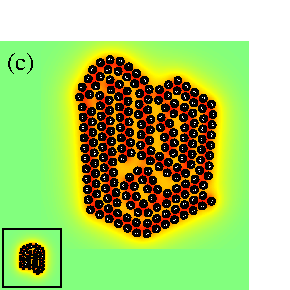
\includegraphics[height=0.3\textheight]{Nb198c_eta_inset.pdf}
  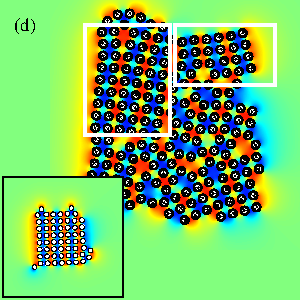
\includegraphics[height=0.3\textheight]{Nb198d_eta_inset.pdf}
\end{center}
\begin{caption}{\label{fig:relax}
  Panel (a) shows $N_b = 198$ particles confined to a square with random
  positions and orientations and the inset shows a $N_b=60$ particles
  configuration. The particles self-assemble into distinct
  configurations, depending on the boundary
  condition~\eqref{eq:bc-type}. Panel (b) is for $b=1$ and the boundary
  condition mimics that of an amphiphilic particle giving bilayer
  structures. Panel (c) is for $b=2$ which gives rise to a
  multilamellar configuration. In panel (d), the case $b = 0$ is for a
  water structure with positive/negative charge. The false color maps
  use blue for $u < 0$, green for $u = 0$, and yellow then red for $u >
  0$. The inset in panels (b)--(d) are configurations using $N_b=60$ and
  share the same color map as the main panels.}
\end{caption}
\end{figure}


Figure~\ref{fig:relax}(a) shows the initial configurations with
orientations of the 198-particle and 60-particle cases, respectively.
BC (i) with $b = 1$ mimics an amphiphilic particle. The boundary data
$g$ is everywhere nonnegative, and takes the maximum value $a$ on the
hydrophobic tail (red) the value $0$ on the hydrophilic head (green).
The interaction is attractive, and particles collectively orient their
hydrophobic sides to form bilayers (Figure~\ref{fig:relax}(b)). The
inset shows the equilibrium state for the 60-particle run. Both
$N_b = 60$ and $N_b = 198$ cases
form bilayers with multiple components.

In BC (ii) with $b = 2$, the boundary data is everywhere positive. It
takes the maximum value $3a$ on the tail (red) and the minimum value $a$
on the head side (yellow). Both sides of the Janus particle are
hydrophobic but more so on the $\alpha = 0$ side. Over a short time
scale, these particles also self-assemble into bilayers. But unlike for
BC (i), the heads are also hydrophobic and so in the long-time dynamics
these bilayers form multilamella structures~\cite{C9NR05885K}. The
number of folds depends primarily on the number of particles.
Figure~\ref{fig:relax}(c), for example, shows a multilamellar structure
with four layers and one with two layers in the inset.

Finally, BC (iii) with $b=0$ corresponds to a water structure with
positive/negative charge~\cite{MaRa76, Ma77}. Here, the head repels the
tail of other particles and the particles initially form chains with
their directors perpendicular to the length of the chain. The chains
form stria where the particles lie on a square grid and the orientations
alternate between layers (Figure~\ref{fig:relax}(d)).

\begin{figure}
  \begin{center}
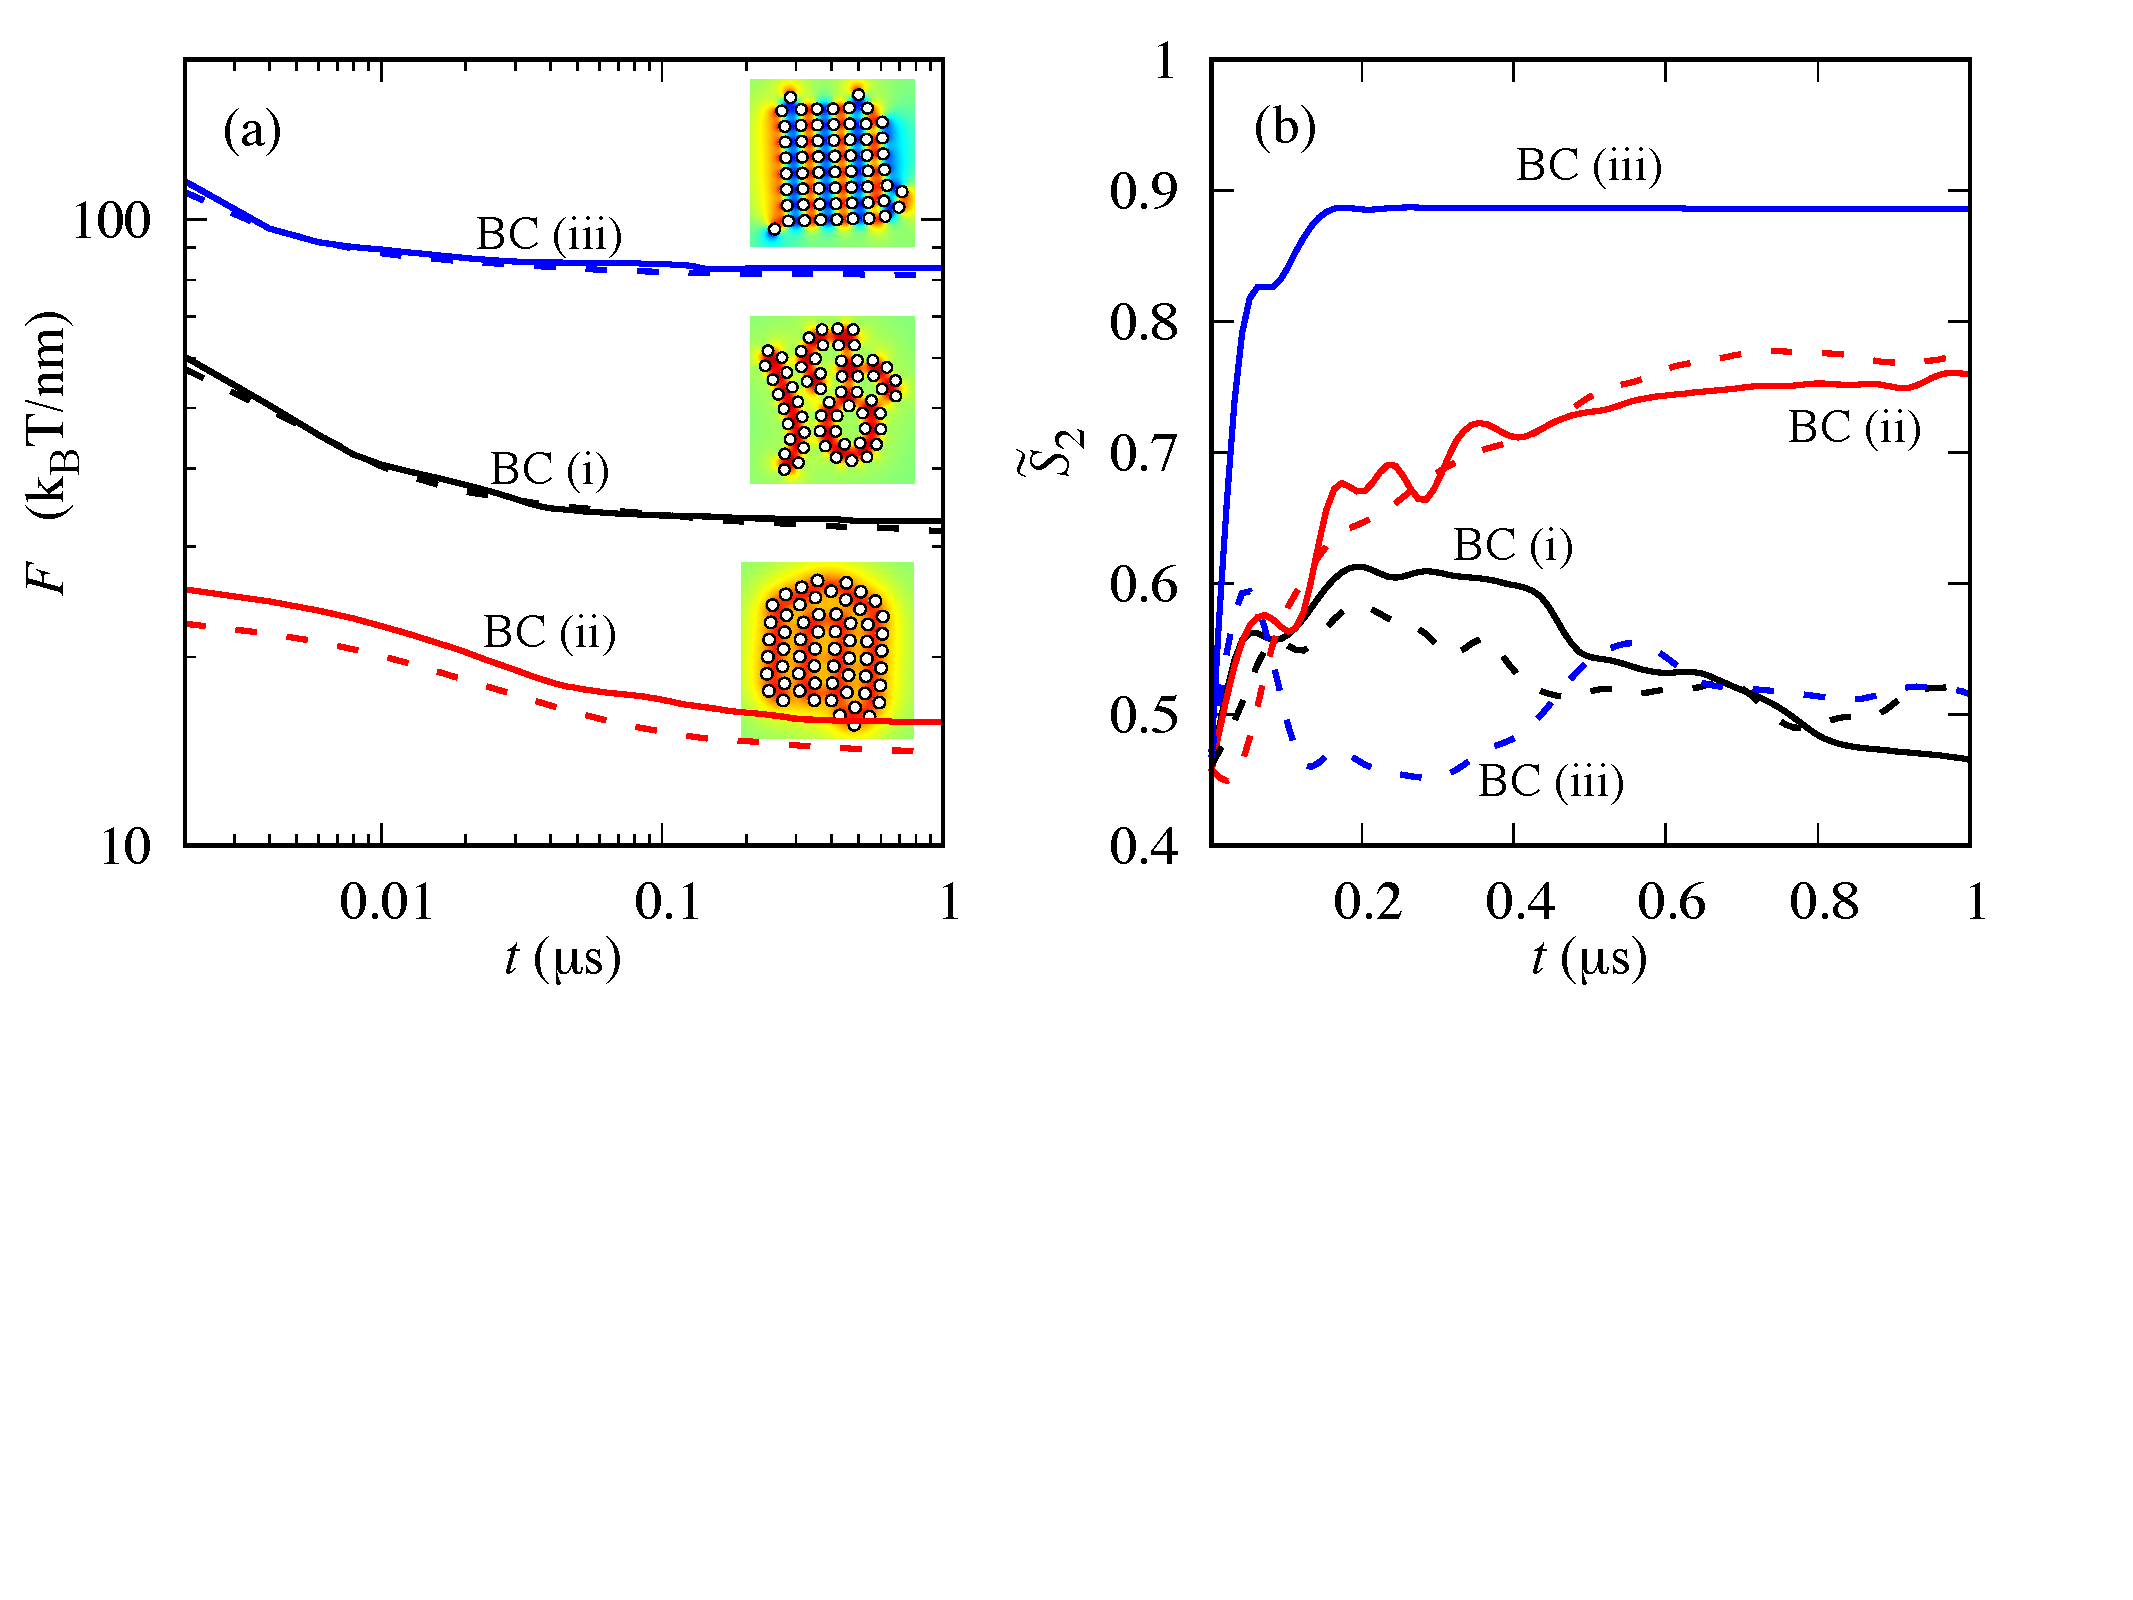
\includegraphics[width=1.0\textwidth]{Figures/Figure2.pdf}
  \end{center}
  \vspace{-20pt}
  \caption{\label{fig:relax_energy}
  Panel (a) shows that the free energy~\eqref{eq:free_energy} decreases
  in the mobility problem formulation. The initial energies are for the
  configuration in Figure~\ref{fig:relax}(a) and the final energies are
  for the near-equilibrium configurations shown in
  Figures~\ref{fig:relax}(b)--(d). The solid curves are the energies for
  the $N_b=60$ cases and the dashed curves are the energies for the $N_b
  = 198$ cases normalized by $60/198$, showing that the energy
  approximately scales with the number of particles.  Panel (b) shows
  the orientational parameters $\tilde{S}_2$ for all 6 relaxation runs.
  The curve styles are identical those in panel (a). The
  near-equilibrium configurations depend on the initial configurations
  and the results show that for both $N_b=60$ and $N_b=198$ cases,
  bilayer and multi-lamellar configurations have similar trends in
  orientational parameters. The results of the striated configuration,
  however, depend on the initial geometrical setup.}
\end{figure}

\section{Measuring deformation}
We use the free energy $F$, a strain parameter $E$, and two scalar order
parameters $S_{2}$ and $\tilde S_2$ to measure the deformation of
particle configurations under background flows. 

First we simplify the form of the free energy~\eqref{eq:free_energy}.
Using integration by parts and~\eqref{eq:SL}, we obtain
\begin{equation}
\label{eq:free_energy2}
F = -\gamma
\int_{\Gamma} \rho g \nabla u \cdot \nnu \,\dif s
+ \frac{M}{2}
\sum_{j \neq i} 
P\left(\frac{|\aa_i - \aa_j|-2c}{\rho_0}\right).
\end{equation}
%
Here, we have substituted $g$ for $u$ since the boundary values are
given. However, evaluating $\nabla u \cdot \nnu$ on $\Gamma$ based
on~\eqref{eq:SL_BIE} involves calculating a quadruple layer potential
which has a well-known obstacle in numerical implementation.  To
overcome this obstacle, we use
%
\begin{equation}
\label{eq:normal_deriv}
\nabla u(\xx) \cdot \nnu(\xx)=
%\frac{\partial}{\partial \nnu_\xx} \DD[\sigma](\xx) =
-\frac{1}{\rho^2} {\bf t}_\xx\cdot \SSS[\sigma{\bf t}](\xx)
+ \frac{\dif}{\dif s}\SSS\left[\frac{\dif \sigma}{\dif s}\right](\xx), \quad \xx \in \Gamma.
\end{equation}
%
Here, $\tt(\xx)$ is the tangent vector and $\dif/\dif s$ is the
arclength derivative. See the Appendix in \S\ref{sec:appendix} for the
proof and details. Substituting~\eqref{eq:normal_deriv}
into~\eqref{eq:free_energy2} for the normal derivative leads to the
single layer, $\SS$, which is more straightforward to evaluate and we
compute the arclength derivative using spectrally accurate Fourier
transform. We have validated the form of~\eqref{eq:normal_deriv} by
extrapolating the primal energy~\eqref{eq:free_energy} along test curves
placed slightly outside the particles.

Figure~\ref{fig:relax_energy}(a) tracks the free energy profiles for all
relaxation runs.  For the 198-particle cases, we normalized the energies
by 60/198 and the results show that all energies decrease with good
agreements in all boundary conditions (dashed curves).  This can be
considered as evidence that the free energy per particle with specified
boundary conditions is independent of the total particle number $(N_b)$.

To measure positional order, we use a number, which we call the strain
parameter, 
\begin{equation}
\label{eq:SP}
E = \frac{1}{N_b} \sum_{i=1}^{N_b}
\left\|\frac{1}{2}(\mathsf{F}_i^T \mathsf{F}_i - I)\right\|,
\end{equation}
where $\mathsf{F}_i$ is an approximate deformation gradient at particle
$i$. The argument inside the Frobenius norm $\| \cdot \|$ is the
Green-Lagrange strain tensor. The motivation for~\eqref{eq:SP} is as
follows. For relatively weak background flow strengths, the
near-equilibrium particle configurations behave as an elastic solid.
There is a map $\ff(\xx,t)$ from the reference (equilibrium)
configuration with $\ff(\aa_i(0),t) = \aa_i(t)$ for $i = 1,\ldots,N_b$.
Using linear approximation,
\begin{align}
\aa_j(t) - \aa_i(t) = \ff(\aa_j(0),t) - \ff(\aa_i(0),t)
\approx \nabla \ff(\aa_i(0),t)(\aa_j(0) - \aa_i(0)).
\end{align}
To approximate the deformation gradient $\nabla \ff(\aa_i(0),t)$ we
solve the overdetermined system 
\begin{align}
\aa_j(t) - \aa_i(t) = \mathsf{F}_i(\aa_j(0) - \aa_i(0)),\quad j =
  1,\ldots, N_b,
\end{align}
for $\mathsf{F}_i$ by weighted least squares. The weights $w_i =
\exp(-\|\aa_j(0) - \aa_i(0)\|/4c)$ with particle radius $c$ ensure that
the linear approximation is valid for particles near $\aa_i$.

Finally, we use the scalar order parameter for orientational order:
\begin{equation}
  \label{eq:S2}
S_2 = \frac{1}{N_b} \sum_{i=1}^{N_b} \frac{1}{2}(3\cos^2(\theta_i - \bar \theta) - 1).
\end{equation}
Here $\bar \theta$ is a circular mean defined as the orientation of the
principal eigenvector of the matrix $\dd_1\dd_1^\top + \cdots +
\dd_{N_b}\dd_{N_b}^\top$. A value $S_2(t) = 1$ indicates that all
particle directors lie on a common axis e.g., two parallel vectors with
possibly opposite direction are ordered. A value far from 1 indicates
disorder.

We modify $S_2$ to account for the bilayer and multilamellar structures.
In these cases, the directors are more or less uniformly distributed
along a circle, even though there is orientational order between
neighboring particles. To account for local order, we instead use
\begin{equation}
  \label{eq:localS2}
\tilde{S}_2(t) = \frac{1}{N_b} \sum_{i=1}^{N_b}
\frac{1}{2}(3\cos^2(\theta_i - \bar \theta_i) - 1),
\end{equation}
where $\bar \theta_i$ is the circular mean restricted to particles
indexed by $j$ with $\|\aa_i - \aa_j\| < 4c$.
This cutoff distance was chosen empirically
so that the average includes nearest neighbors
but excludes next nearest neighbors.
In practice, if a particle
is isolated and has no neighbors within a distance $4c$, then we exclude
it from the sum~\eqref{eq:localS2}. 

Figure~\ref{fig:relax_energy}(b) tracks the orientational order
parameter $\tilde{S}_2$. Both bilayer and multilamellar structures show
similar trends in the small and large particle number systems
(Figure~\ref{fig:relax_energy}(b) black curves and red curves,
respectively). The multilamellar structures are highly ordered in all
cases (Figure~\ref{fig:relax}(c)) whereas the bilayer structures are
disordered because they consist of several components forming isolated
bilayers, micelles, and vesicles (Figure~\ref{fig:relax}(b)).

The aggregation for striated configurations forms more than one pattern
when the number of particles is varied (Figure~\ref{fig:relax}(d)). We
observe that when the number of particles is fewer, there is only a
single pattern in particle orientations where the directors are more or
less parallel and alternate directions (Figure~\ref{fig:relax}(d),
inset). Larger number of particles results in two different patterns:
the alternating sign pattern as in the small particle number case
(Figure~\ref{fig:relax}(d), top right rectangle) and one where the
directors reflect across the lines parallel to the stria and across the
lines perpendicular to the stria (Figure~\ref{fig:relax}(d), top middle
rectangle). As a result, there are different trends in orientational
order (Figure~\ref{fig:relax_energy}(b), solid and dashed blue curves,
respectively).

In the Results section, the equilibrium configurations for BCs (i),
(ii), and (iii) (Figure~\ref{fig:relax}, insets) are used as initial
data in the background flow simulations. For the bilayer case BC (i),
we include an alternate initial condition consisting of a single,
circular vesicle (c.f., Figure~\ref{fig:Ves_shear}).


%%%%%%%

\begin{figure}
  \begin{center}
   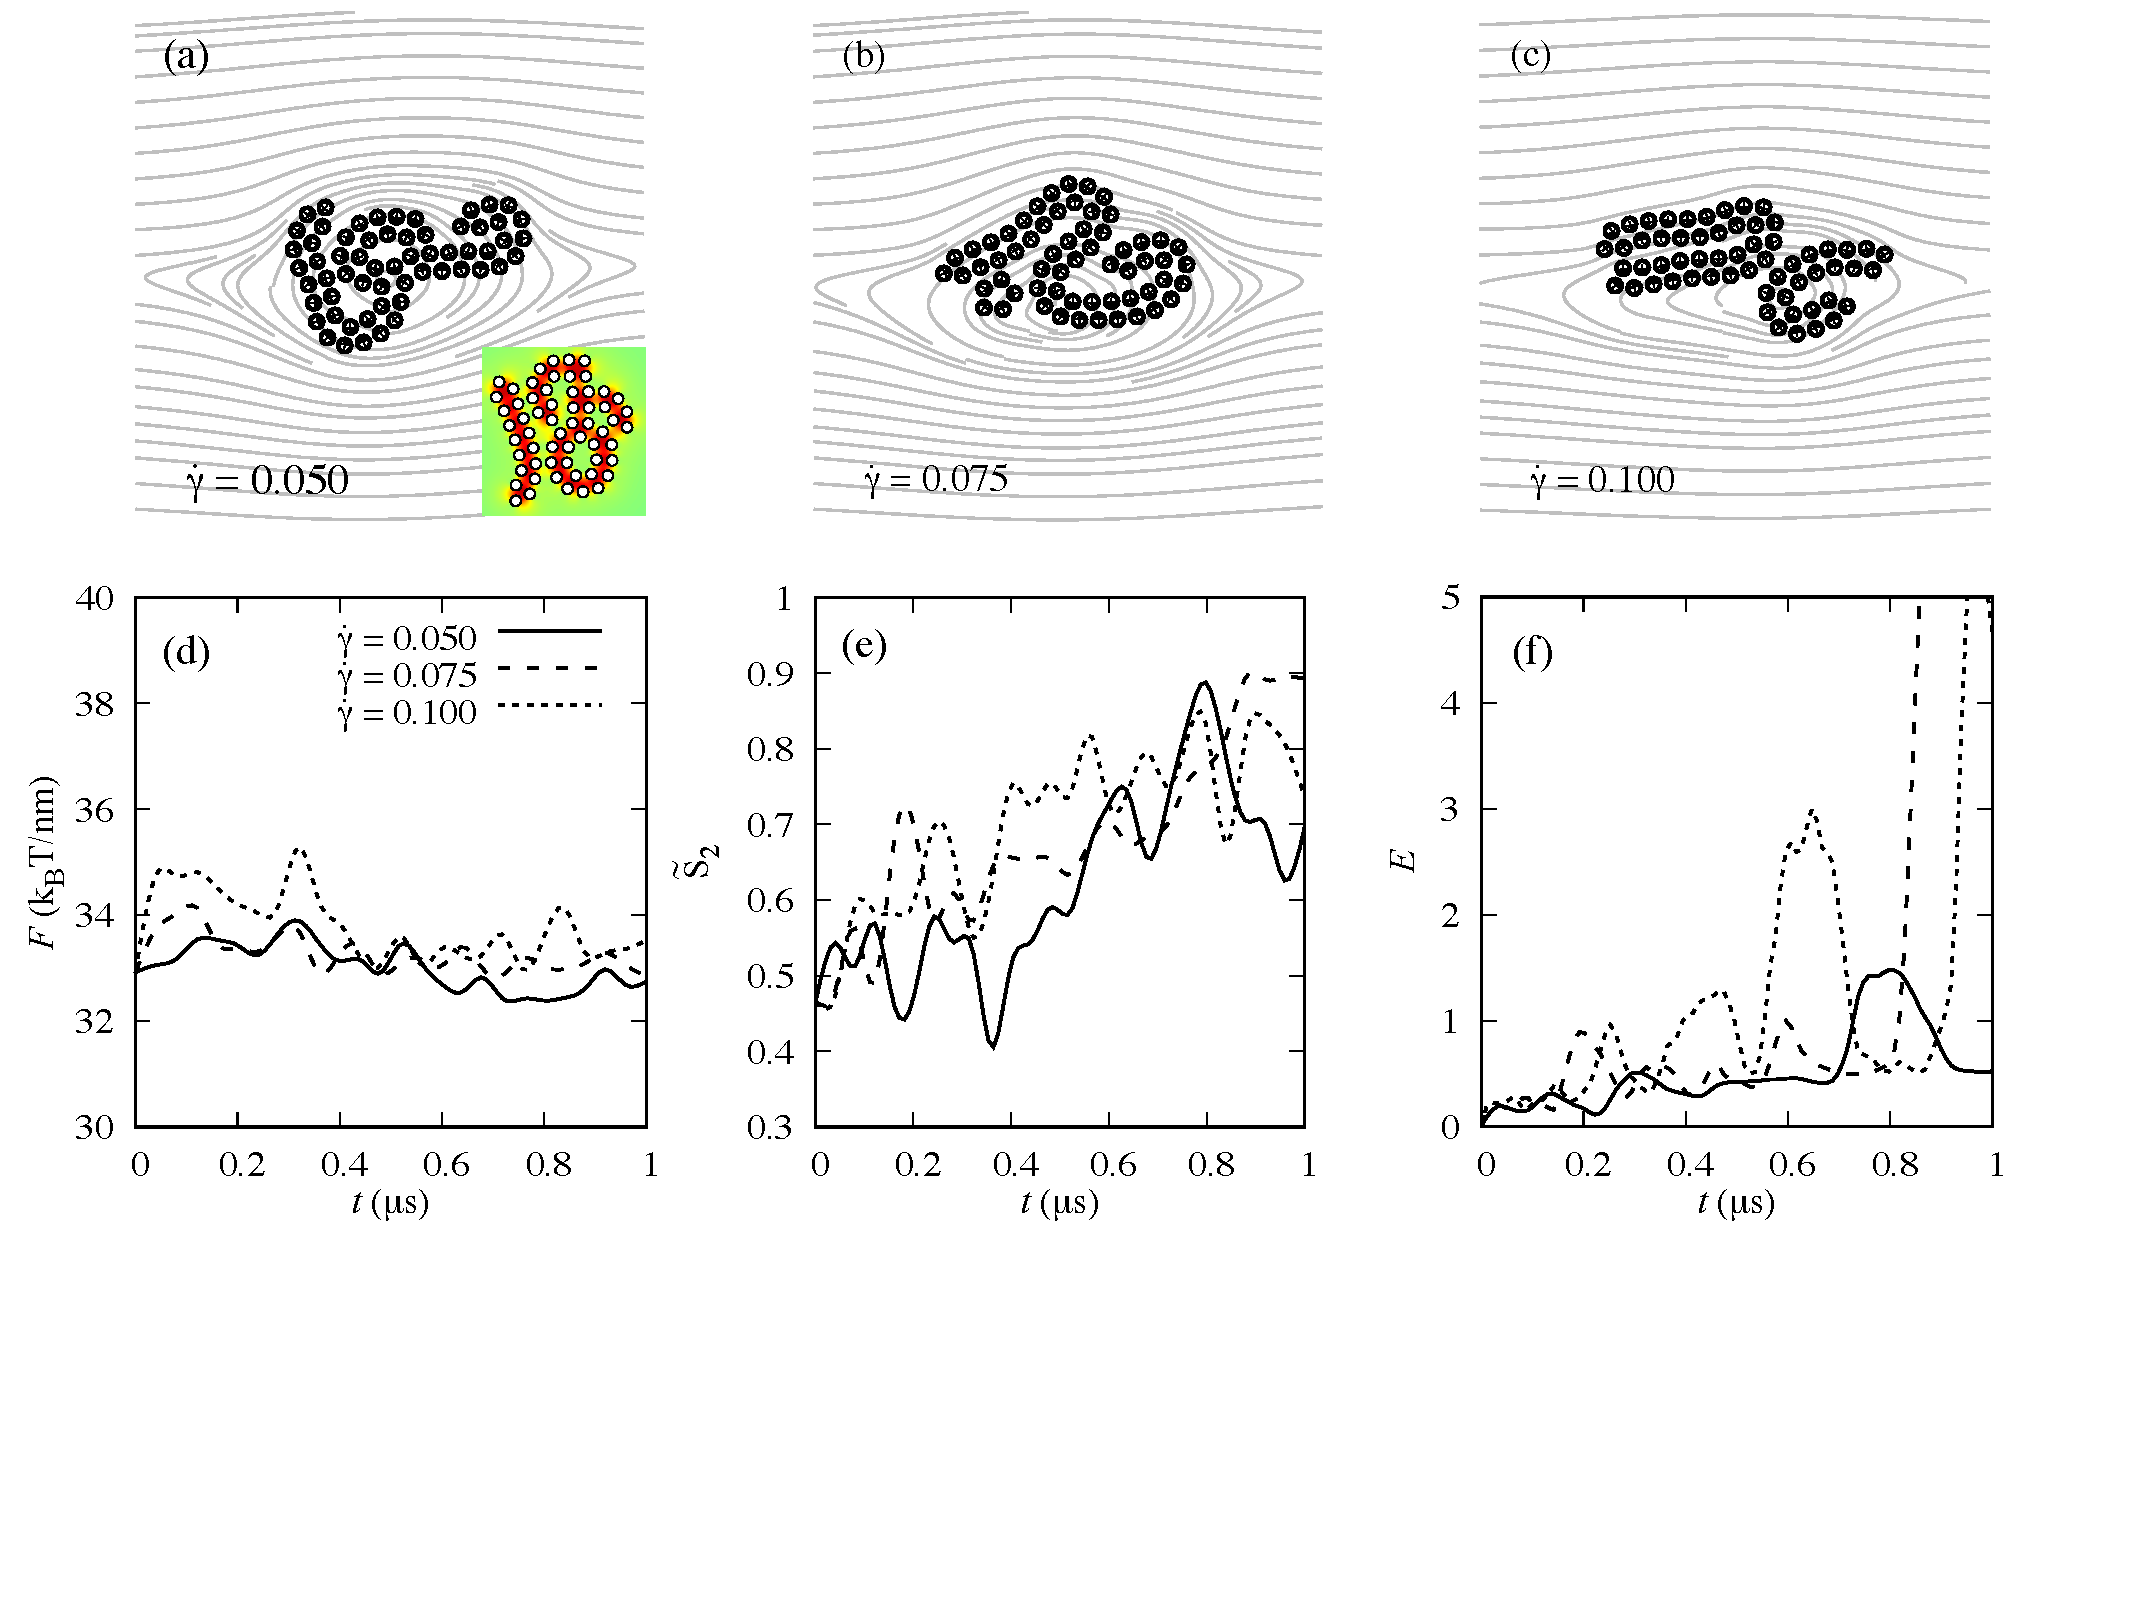
\includegraphics[width=1.0\textwidth]{Figures/Figure3.pdf}
  \end{center}
  \caption{
    \label{fig:BC1_shear}
    Panels (a)--(c) are a snapshot at $t=0.5\ \upmu$s of the
    multiple-component bilayer with shear rate $\dot \gamma = \{0.05,
    0.075, 0.1\}$. The initial configuration is shown in inset of panel
    (a). The streamlines are plotted in the background. Panel (d) shows
    the free energies, panel (e) shows the orientational parameter
    $\tilde{S}_2$, and panel (f) shows positional parameter E.}
\end{figure}



\section{Results}
\label{sec:results}
In this section, we subject the JP structures to various
background flows. The purpose is to understand how the self-assemblies
respond to external forcing. We then compare effective
properties of materials comprised of JPs as a function of
their amphiphilic properties.
%%%

\subsection{Bilayer configurations (BC (i)) in a linear shear flow}
To begin, we place the bilayer structure (with BC (i)) from the inset of
Figure~\ref{fig:relax}(b) in a linear shear flow
\begin{equation}
\uu_\infty(\xx) = \dot\gamma \text{ ns }^{-1} ({\bf e}_y \cdot \mathbf{x}) {\bf e}_x,
\end{equation}
%
where $\dot\gamma$ is the dimensionless shear rate, and ${\ee}_x$ and
${\ee}_y$ are horizontal and vertical unit vectors, respectively. The
initial bilayer structure consists of a small self-enclosing bilayer
(vesicle) and several pieces of bilayers.
Figure~\ref{fig:BC1_shear}(a)--(c) shows a snapshot at $t = 0.5$
$\upmu$s of the bilayer for different shear rates $\dot\gamma=
0.05,0.075,0.01$. The dynamics of the bilayer can be found in
Supplementary Movie S2, which shows
that the initial pieces of bilayers
merge and form a worm-like shape under a linear shear flow. At a low
shear rate, the bilayer constantly goes through rotation and extensional
deformation with the whole bilayer remaining intact
(Figure~\ref{fig:BC1_shear}(a)). As the shear rate increases to a
moderate value (Figure~\ref{fig:BC1_shear}(b)), the bilayer is observed
to shed a small piece of bilayer, similar to the asymmetric breakup of a
viscous drop in confinement \cite{DuFuZhuMaLi2016_AICHEJ}.
%\todo[inline]{missing citation}. 
In Figure~\ref{fig:BC1_shear}(c) the high shear rate gives rise to two
separate, nearly equal bilayers, similar to the symmetric drop breakup
under a linear shear flow \cite{Stone1994_ARFM}. 
Refer to Supplementary Movie S4.

%\todo[inline]{missing citation}.
%%
%\begin{figure}
%  \begin{center}
%    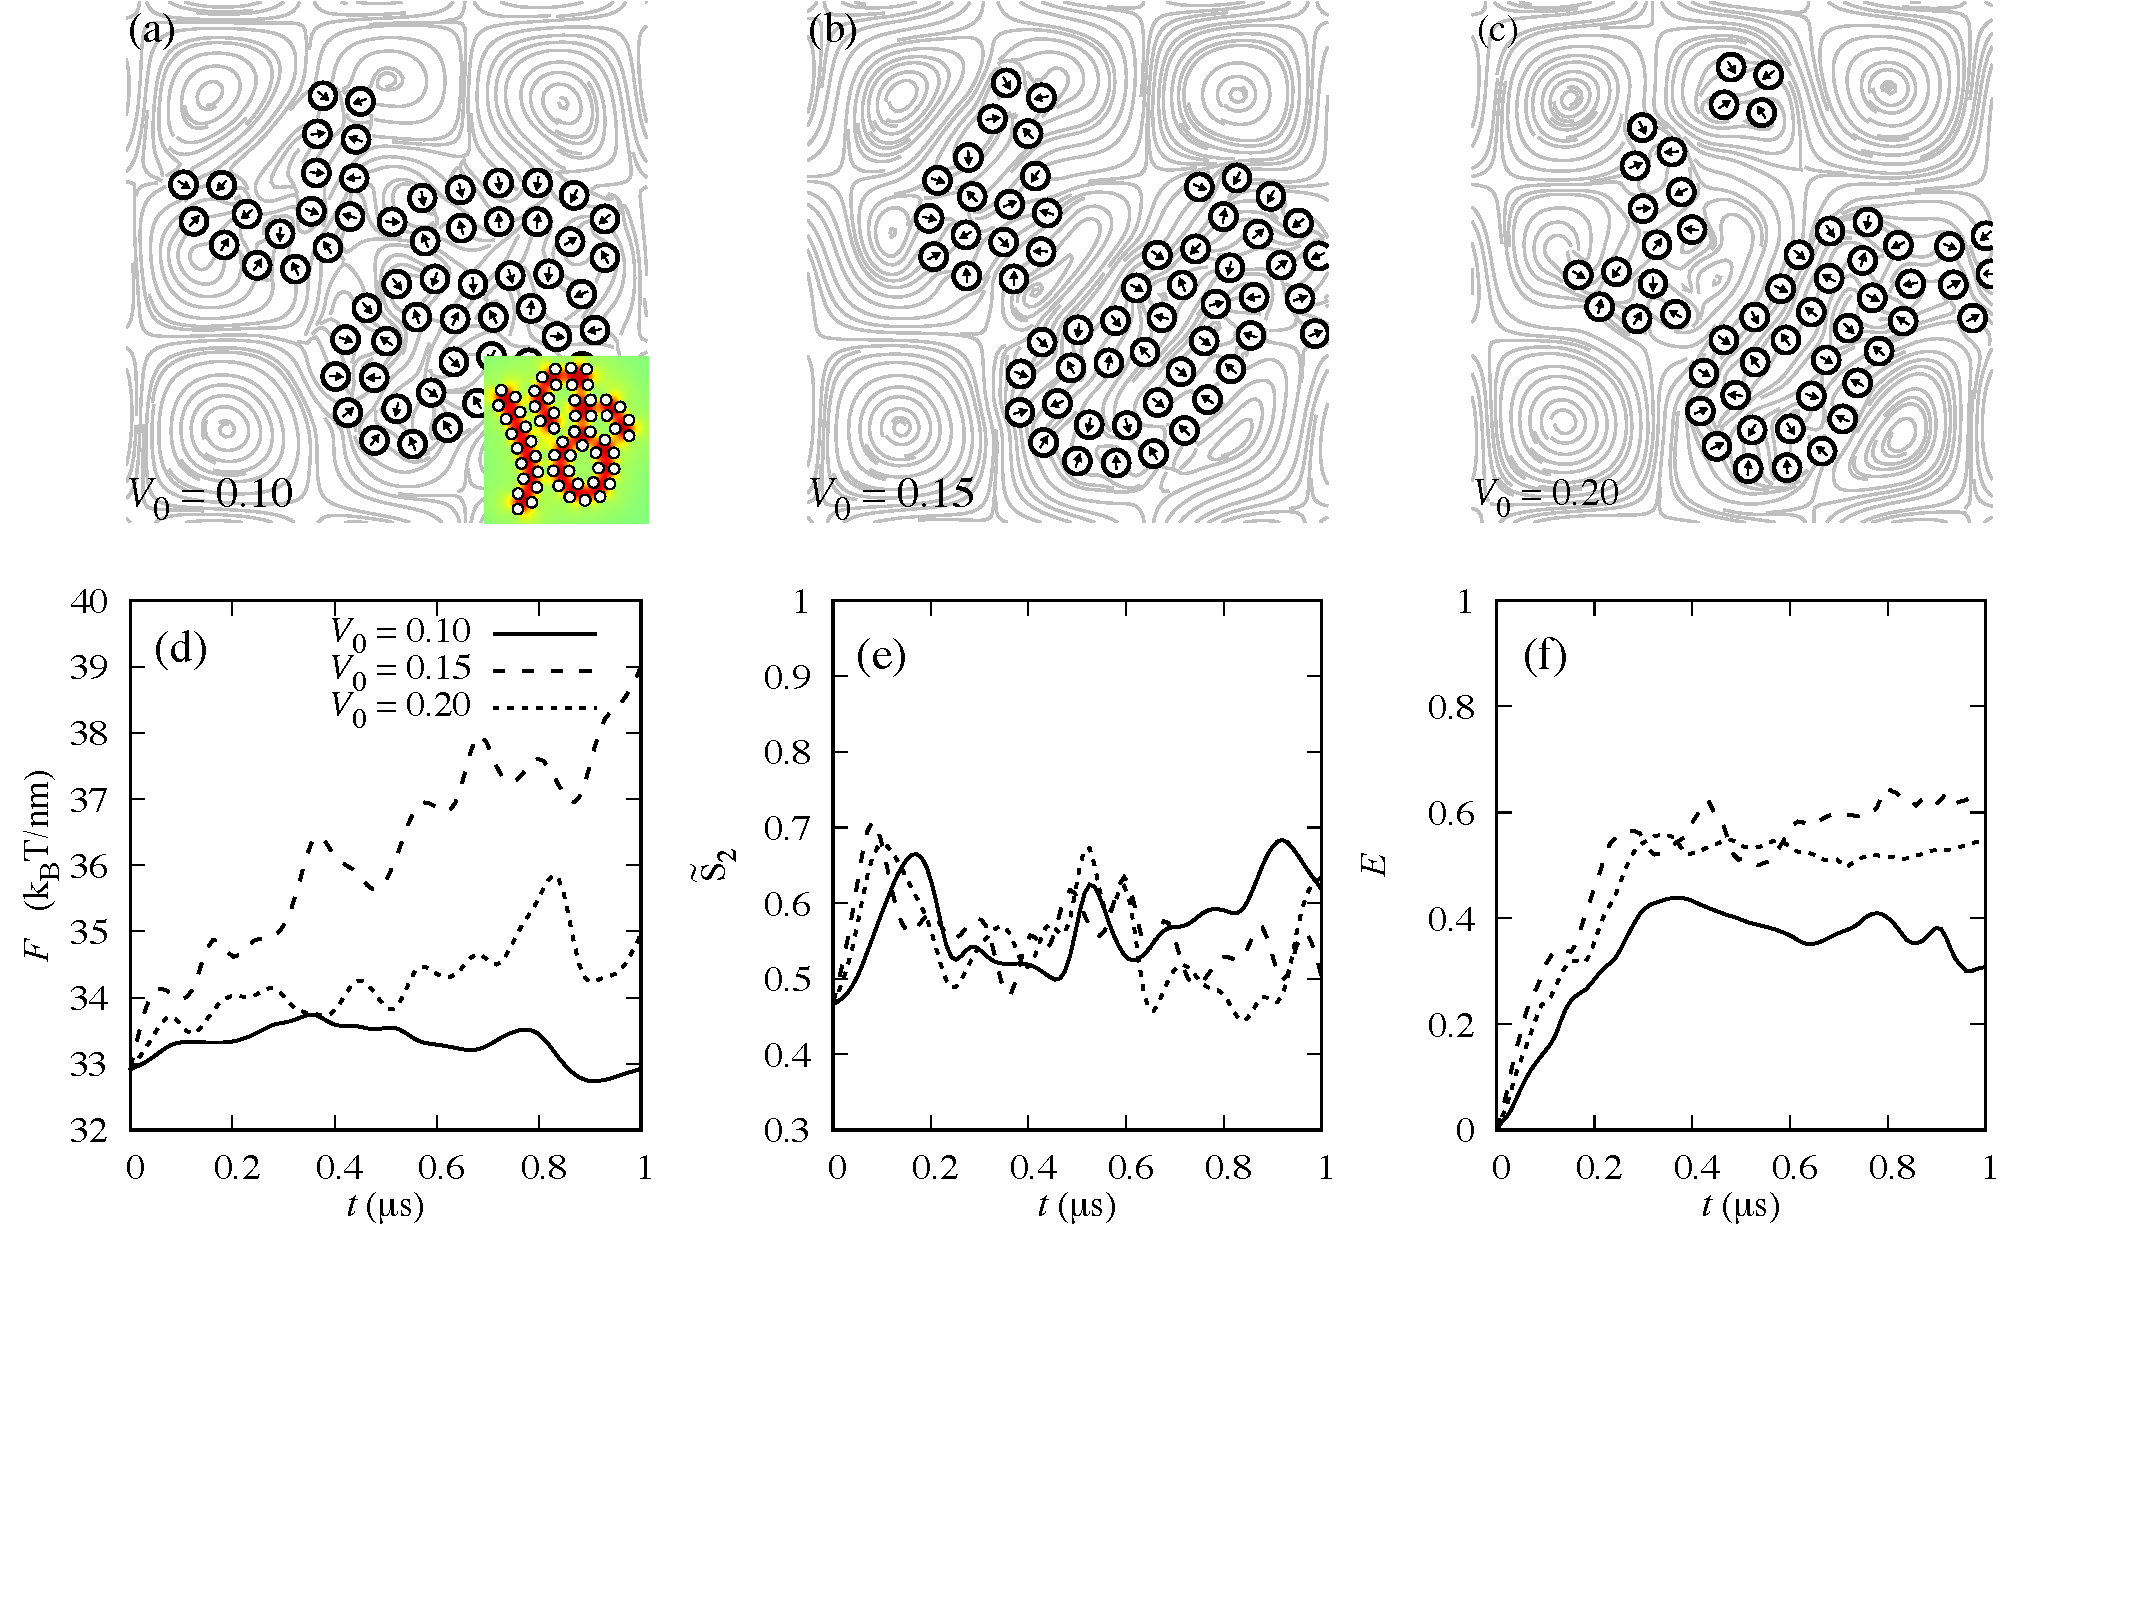
\includegraphics[width=1.0\textwidth]{Figures/Figure5.pdf}    
%  \end{center}
%  \vspace{-20pt}  
%  \caption{\label{fig:BC1_TG} Multiple component bilayers in a Taylor-Green when $V_0 = \{0.1, 0.15, 0.2\}$ at $t=0.2\ \mu$s. The pre-relaxed initial configuration is shown in inset of panel (a). 
% The streamlines are plotted in the background. 
%Panel (d) plots the free energies; panel (e) shows orientational parameter $\tilde{S}_2$; panel (f) shows positional parameter E.
%  }
%\end{figure}

We observe that the order parameter $\tilde S_2$ in
Figure~\ref{fig:BC1_shear}(e) is on average increasing. In the initial
configuration, the structure has three or four components.
%
Under the shear flow, the shedding and merging of bilayers results in an
overall decrease in distinct bilayer structures. Similarly, the free
energies are slightly decreasing (Figure~\ref{fig:BC1_shear}(d)), with
the overall changes occurring in the range of a few $\mathrm{k_BT}$/nm.
This suggests that the shear flow changes the energy landscape to move
the local equilibrium obtained from a random initial condition to an
alternate local equilibrium with less free energy and greater
orientational order  (Supplementary Movie S2).  Note that the free energy $F$ in
Figure~\ref{fig:BC1_shear}(d) has the unit of force ($\mathrm{k_BT}$/nm $\approx$ 4.114 pN)
because our system
is two dimensional.
%
%\begin{figure}
%  \begin{center}
%    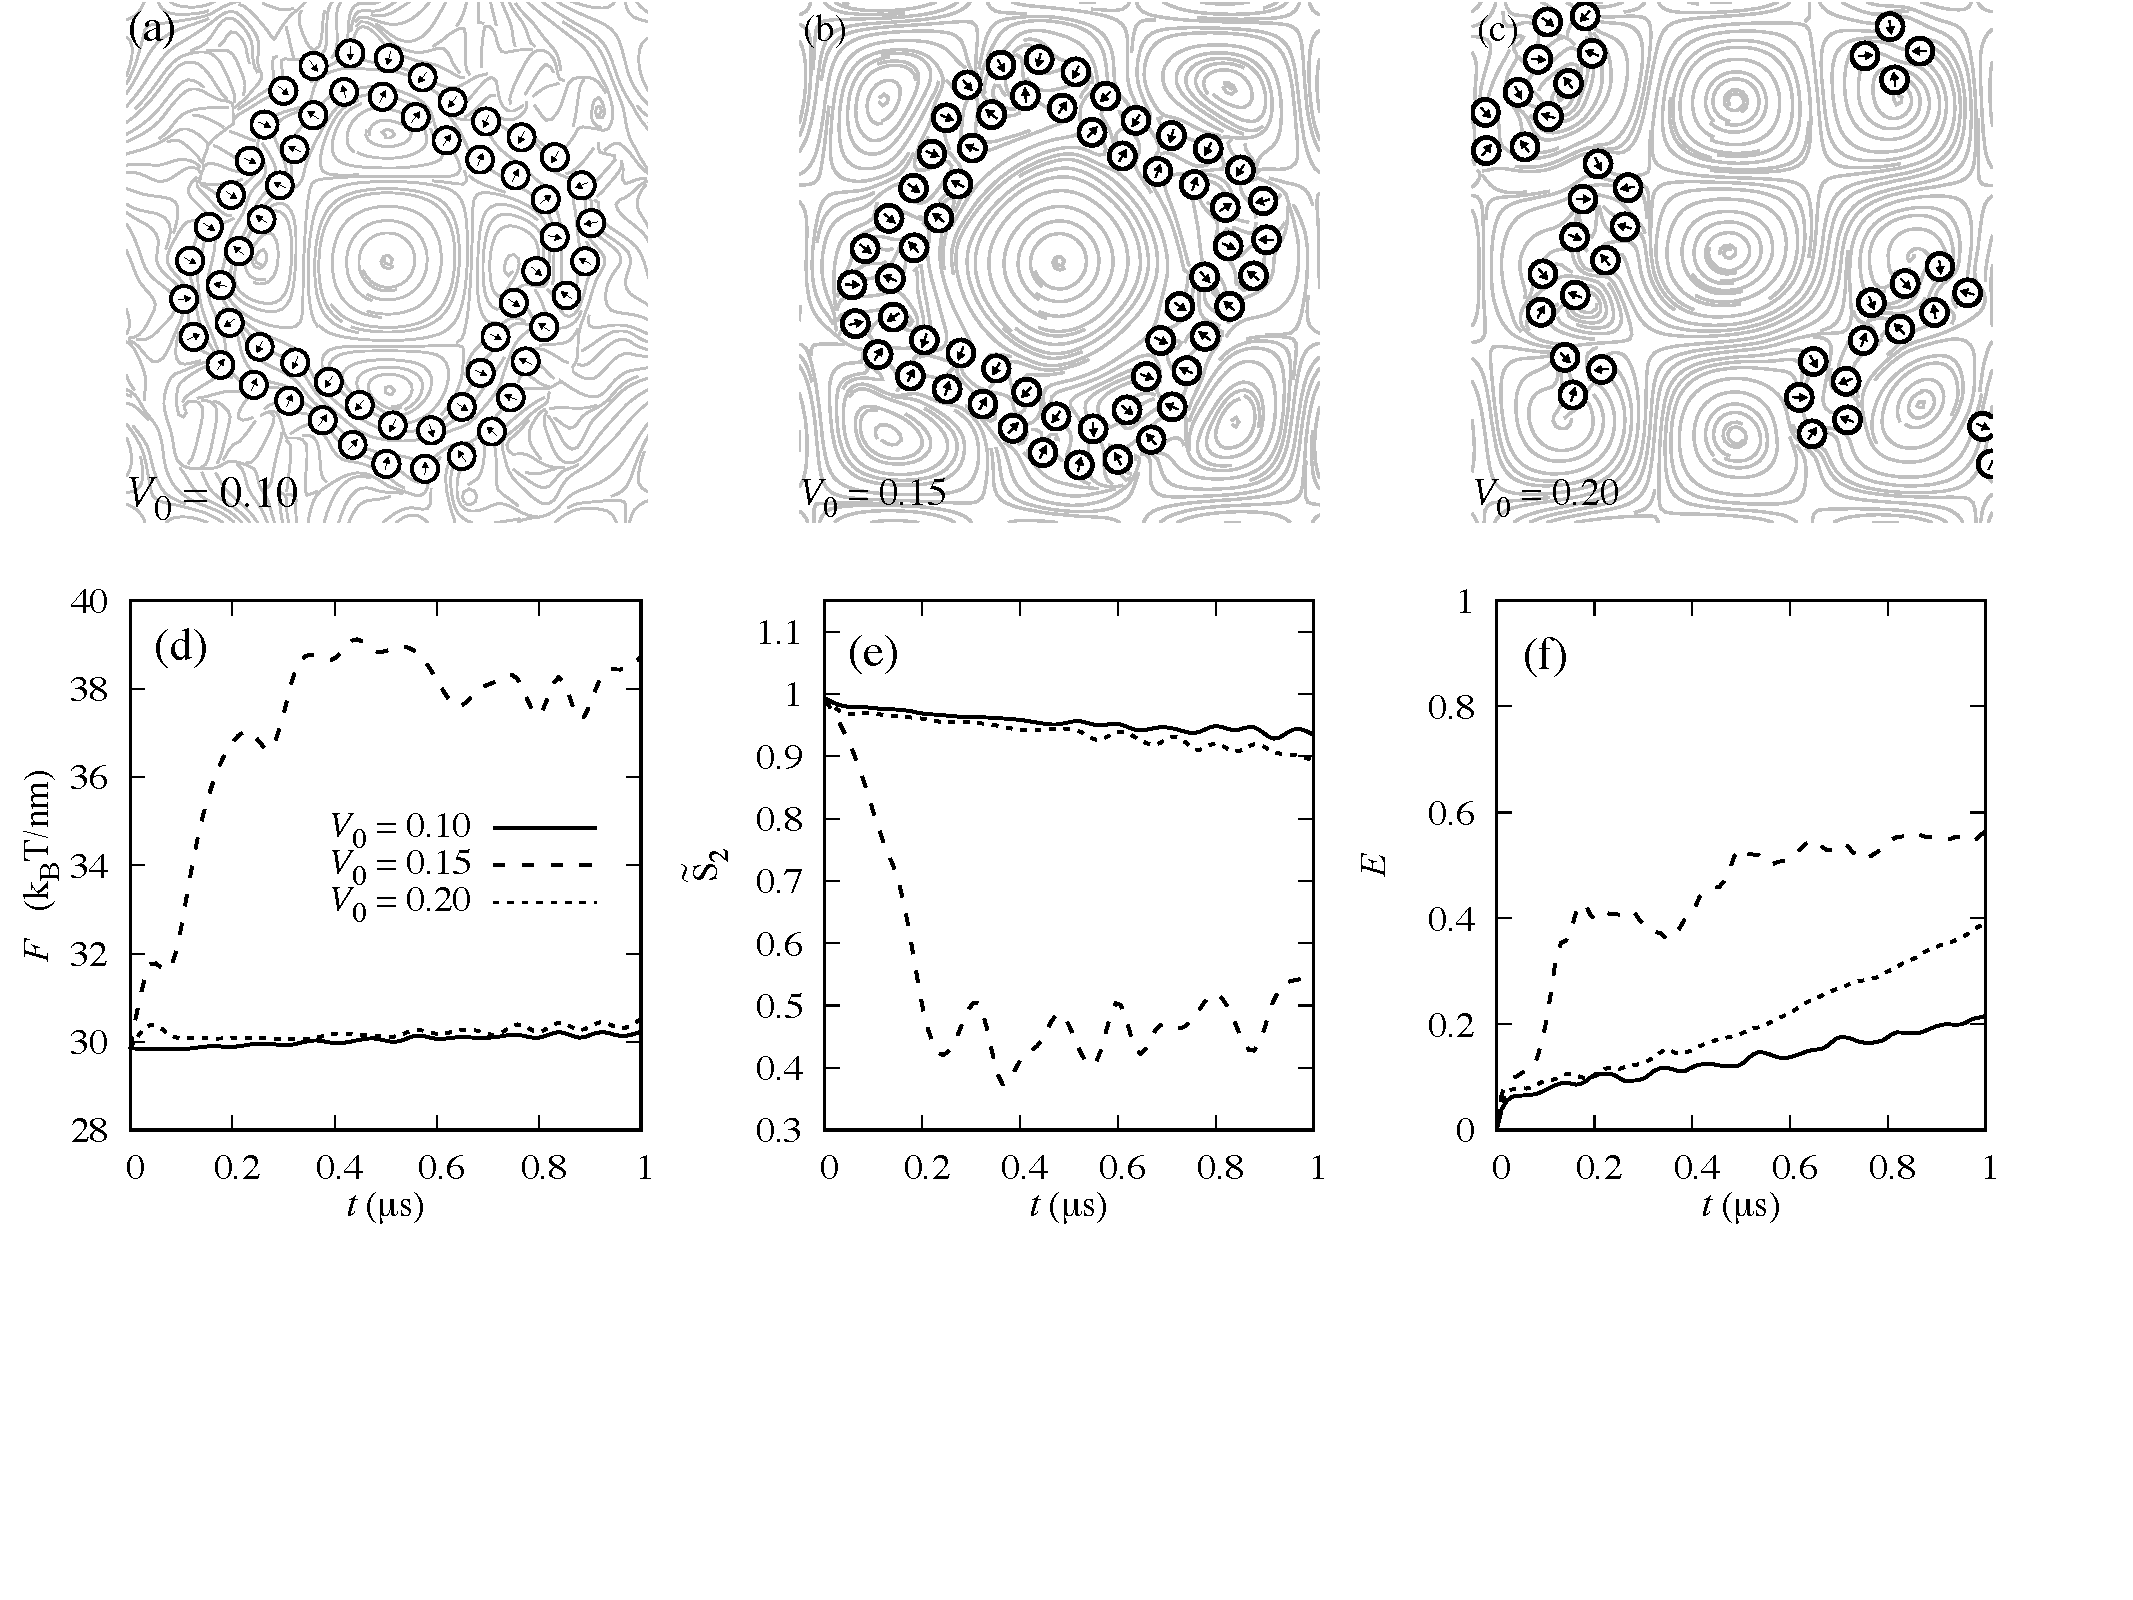
\includegraphics[width=1.0\textwidth]{Figures/Figure6.pdf}        
%  \end{center}
%\caption{\label{fig:ves_TG} Single vesicle in a TG flow. Panels (a)-(c) are snapshots for $V_0=\{0.1, 0.15, 0.2\}$ at $t=0.6\ \mu$s where the pre-relaxed initial configuration is shown in inset of panel (a). The streamlines are plotted in the background.
%Panel (d) plots the free energies; panel (e) shows orientational parameter $\tilde{S}_2$; panel (f) shows positional parameter E.
%}
%\end{figure}
%
Finally, the strain parameter diverges in the large shear rate cases
(Figure~\ref{fig:BC1_shear}(f))
because the components eventually completely separate and move away from one another
under the shear flow.

%%%
\begin{figure}
  \begin{center}
    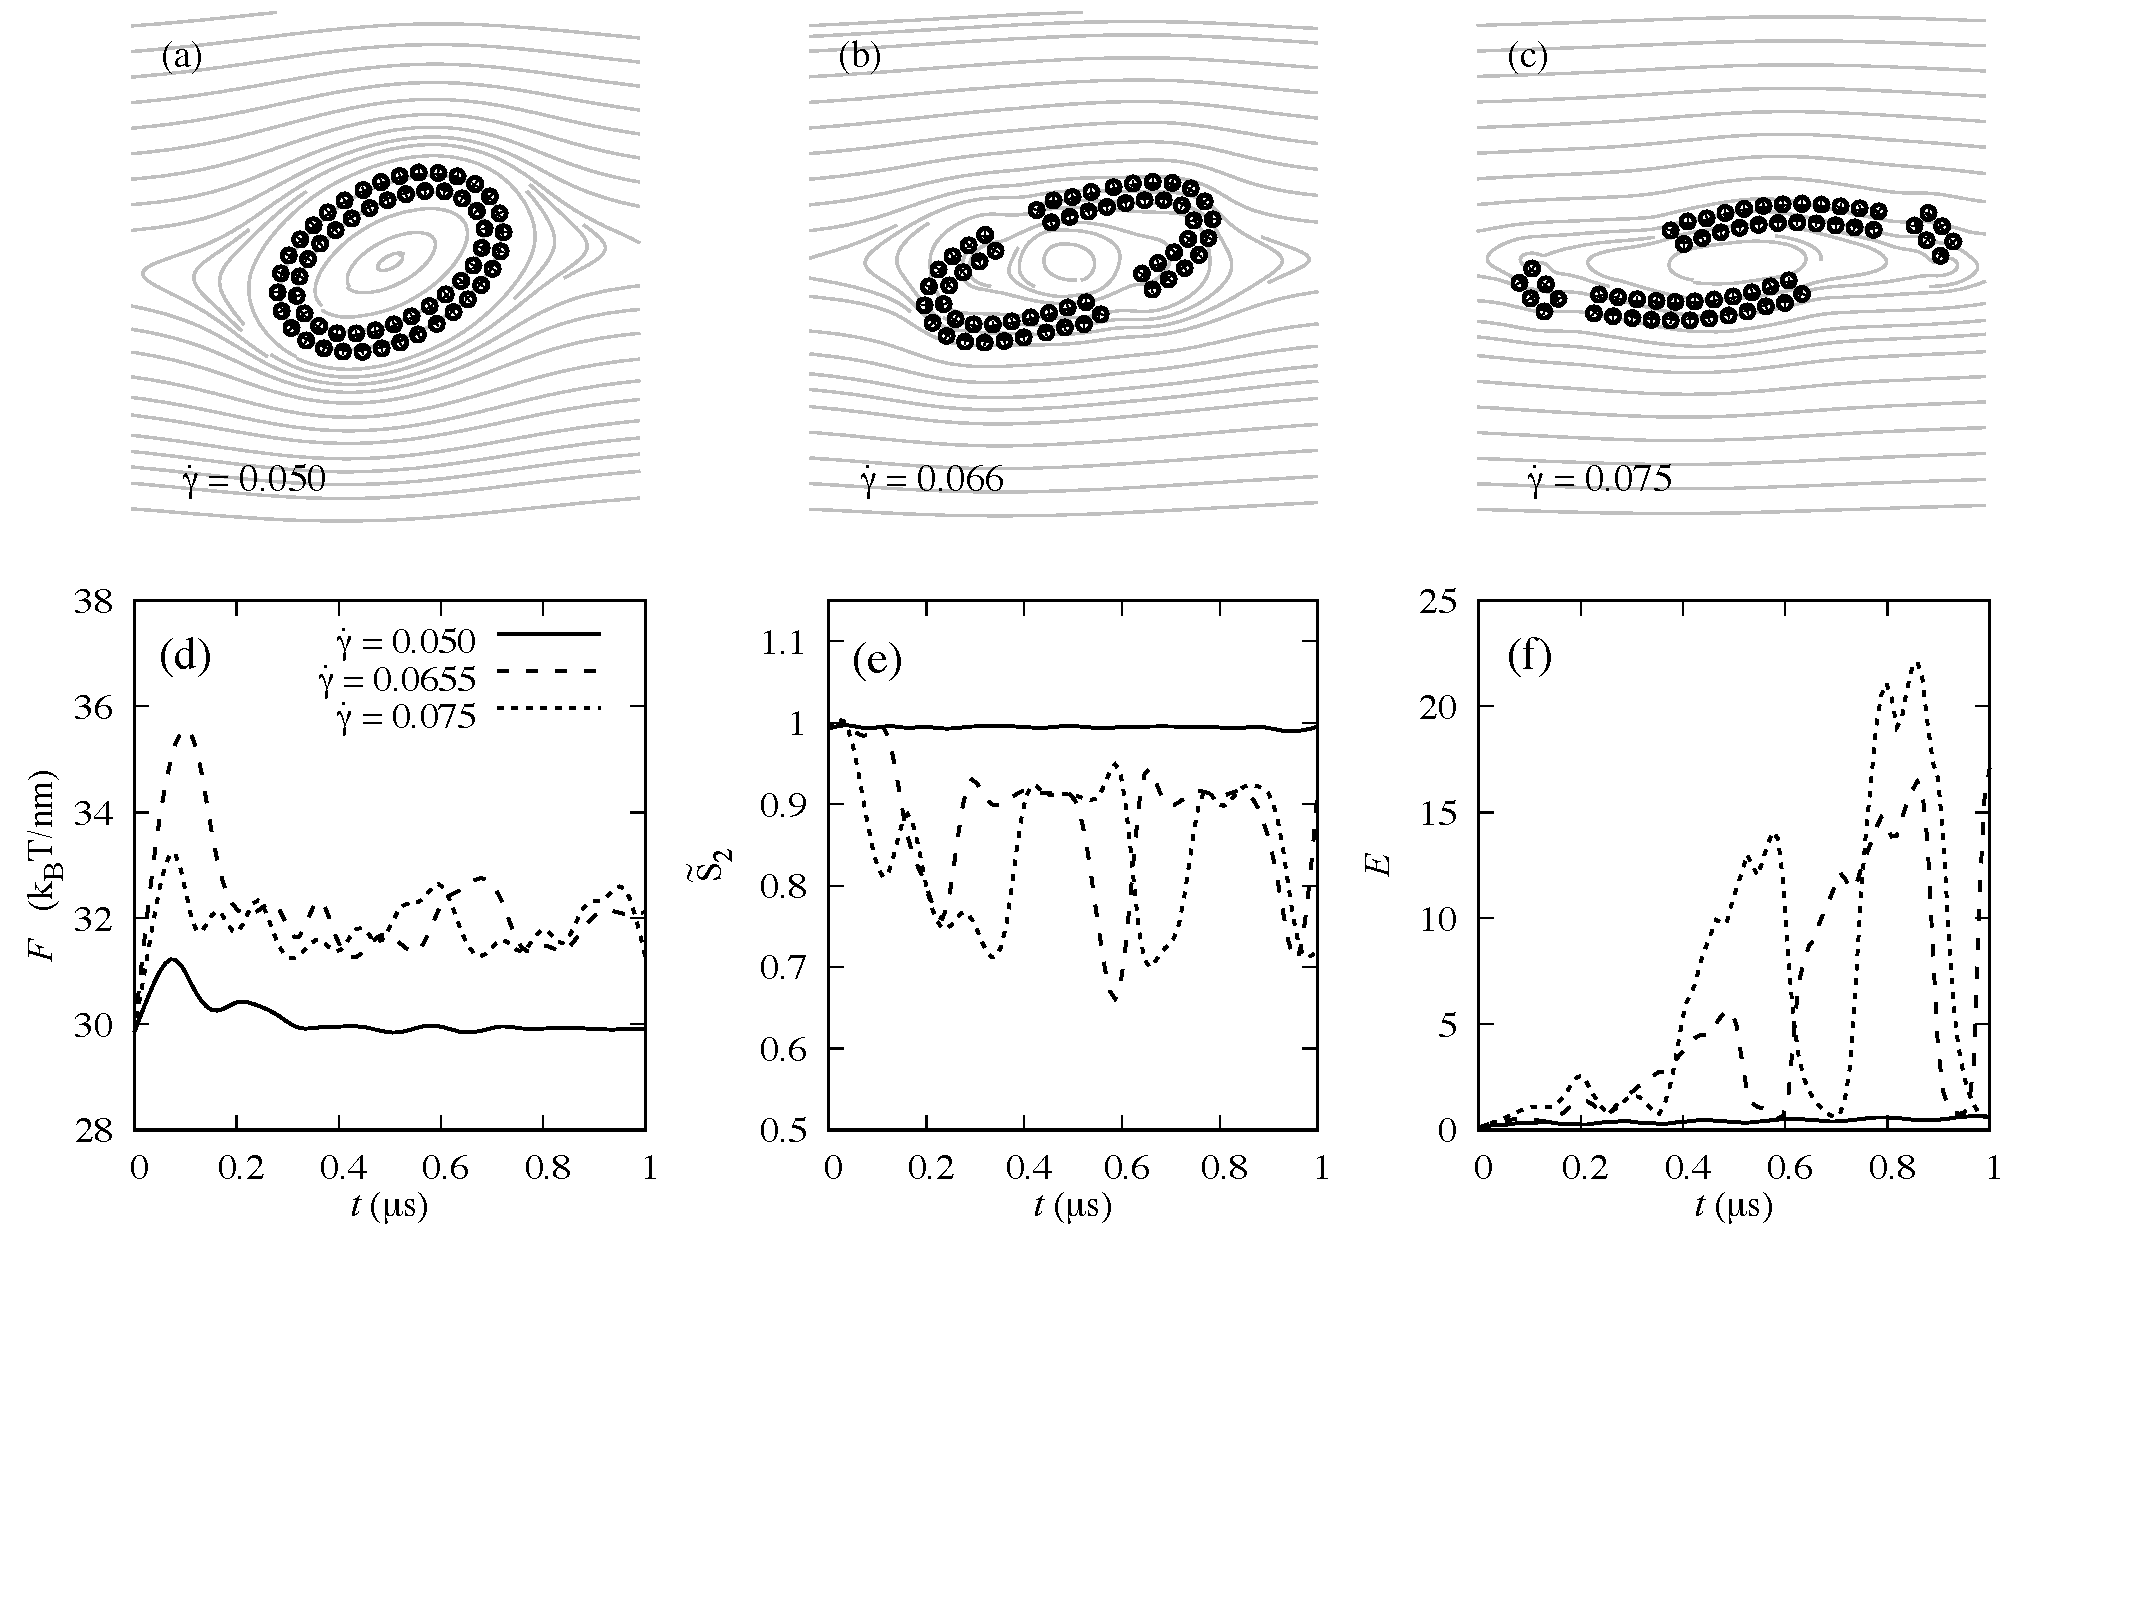
\includegraphics[width=1.0\textwidth]{Figures/Figure4.pdf}
  \end{center}
  \caption{
    \label{fig:Ves_shear}
A single vesicle in a shear flow. Panels (a)--(c) are snapshots for
  $\dot \gamma = \{0.05, 0.0655, 0.075\}$ at $t=0.16\ \upmu$s where the
  pre-relaxed initial configuration is shown in inset of panel (a). The
  streamlines are plotted in the background. Panel (d) shows the free
  energies; panel (e) shows orientational parameter $\tilde{S}_2$; panel
  (f) shows positional parameter E.}
\end{figure}
\citet{Fu2022_JFM} studied the hydrodynamics of a JP vesicle under a
linear shear flow. Focusing on drawing analogies to hydrodynamics of a
vesicle in continuum modeling (such as
tank-treading~\cite{keller_skalak_1982,Finken08,Shaqfeh11}, bilayer
slip~\cite{sch-vla-mik2010,denOtter2007,Zgorski2019}, and
permeability~\cite{chabanon2017, qua-gan-you2021}), our previous work
demonstrated the existence of a critical shear rate above which the JP vesicle
ruptures~\cite{grandmaison_brancherie_salsac_2021,D2SM00179A}. Based on
the these early results, we reinitialized the BC (i) configuration in
the form of a single, circular vesicle (rather than several bilayer
components) and illustrate how the three measures of structural
deformation correlate to the dynamics of a JP vesicle.

At shear rates $\dot\gamma=0.05, 0.066, 0.075$, the vesicle undergoes
familiar hydrodynamics, such as elongation along the extensional axis
and tank-treading motion, as shown in
Figure~\ref{fig:Ves_shear}(a)--(c)
and Supplementary Movie S2.
%
The circular shape is also a local equilibrium, with somewhat less
energy than the disordered state c.f., Figure~\ref{fig:BC1_shear}(d) and
Figure~\ref{fig:Ves_shear}(d). But unlike the dynamics of bilayers in
Figure~\ref{fig:BC1_shear}, the energies of the JP vesicle in
Figure~\ref{fig:Ves_shear}(d) jump from the baseline value 30
$\mathrm{k_BT}$/nm to about 32 $\mathrm{k_BT}$/nm, signaling the rupture
of the vesicle into disconnected bilayers (see
Figure~\ref{fig:Ves_shear}(d), long and short dashed curves).  After the
rupture, each piece circles around the vorticity at the center without
reconnection while the energies fluctuate slightly around a constant.

For the lowest shear rate case, the vesicle has nearly constant
orientational order $\tilde S_2 = 1$ (see Figure~\ref{fig:Ves_shear}(e),
solid curve). After the JP vesicle ruptures with $\dot\gamma= 0.066$ and
$\dot \gamma= 0.075$, we observe a greater variation in the order
parameter $\tilde{S}_2$ with a baseline value around $0.7$ (see
Figure~\ref{fig:Ves_shear}(e), dashed curves). The oscillations occur
due to the orbit of the two bilayer components, and $\tilde{S}_2$
increases to about $0.9$ when the components slide past one another and
are nearly parallel.
%
As in the previous case, peaks in the strain parameter $E$ correlate
well with changes in structural topology in the bilayer dynamics (dashed
curves in Figure~\ref{fig:Ves_shear}(f)).


%%%%%%%
%
\begin{figure}
  \begin{center}
    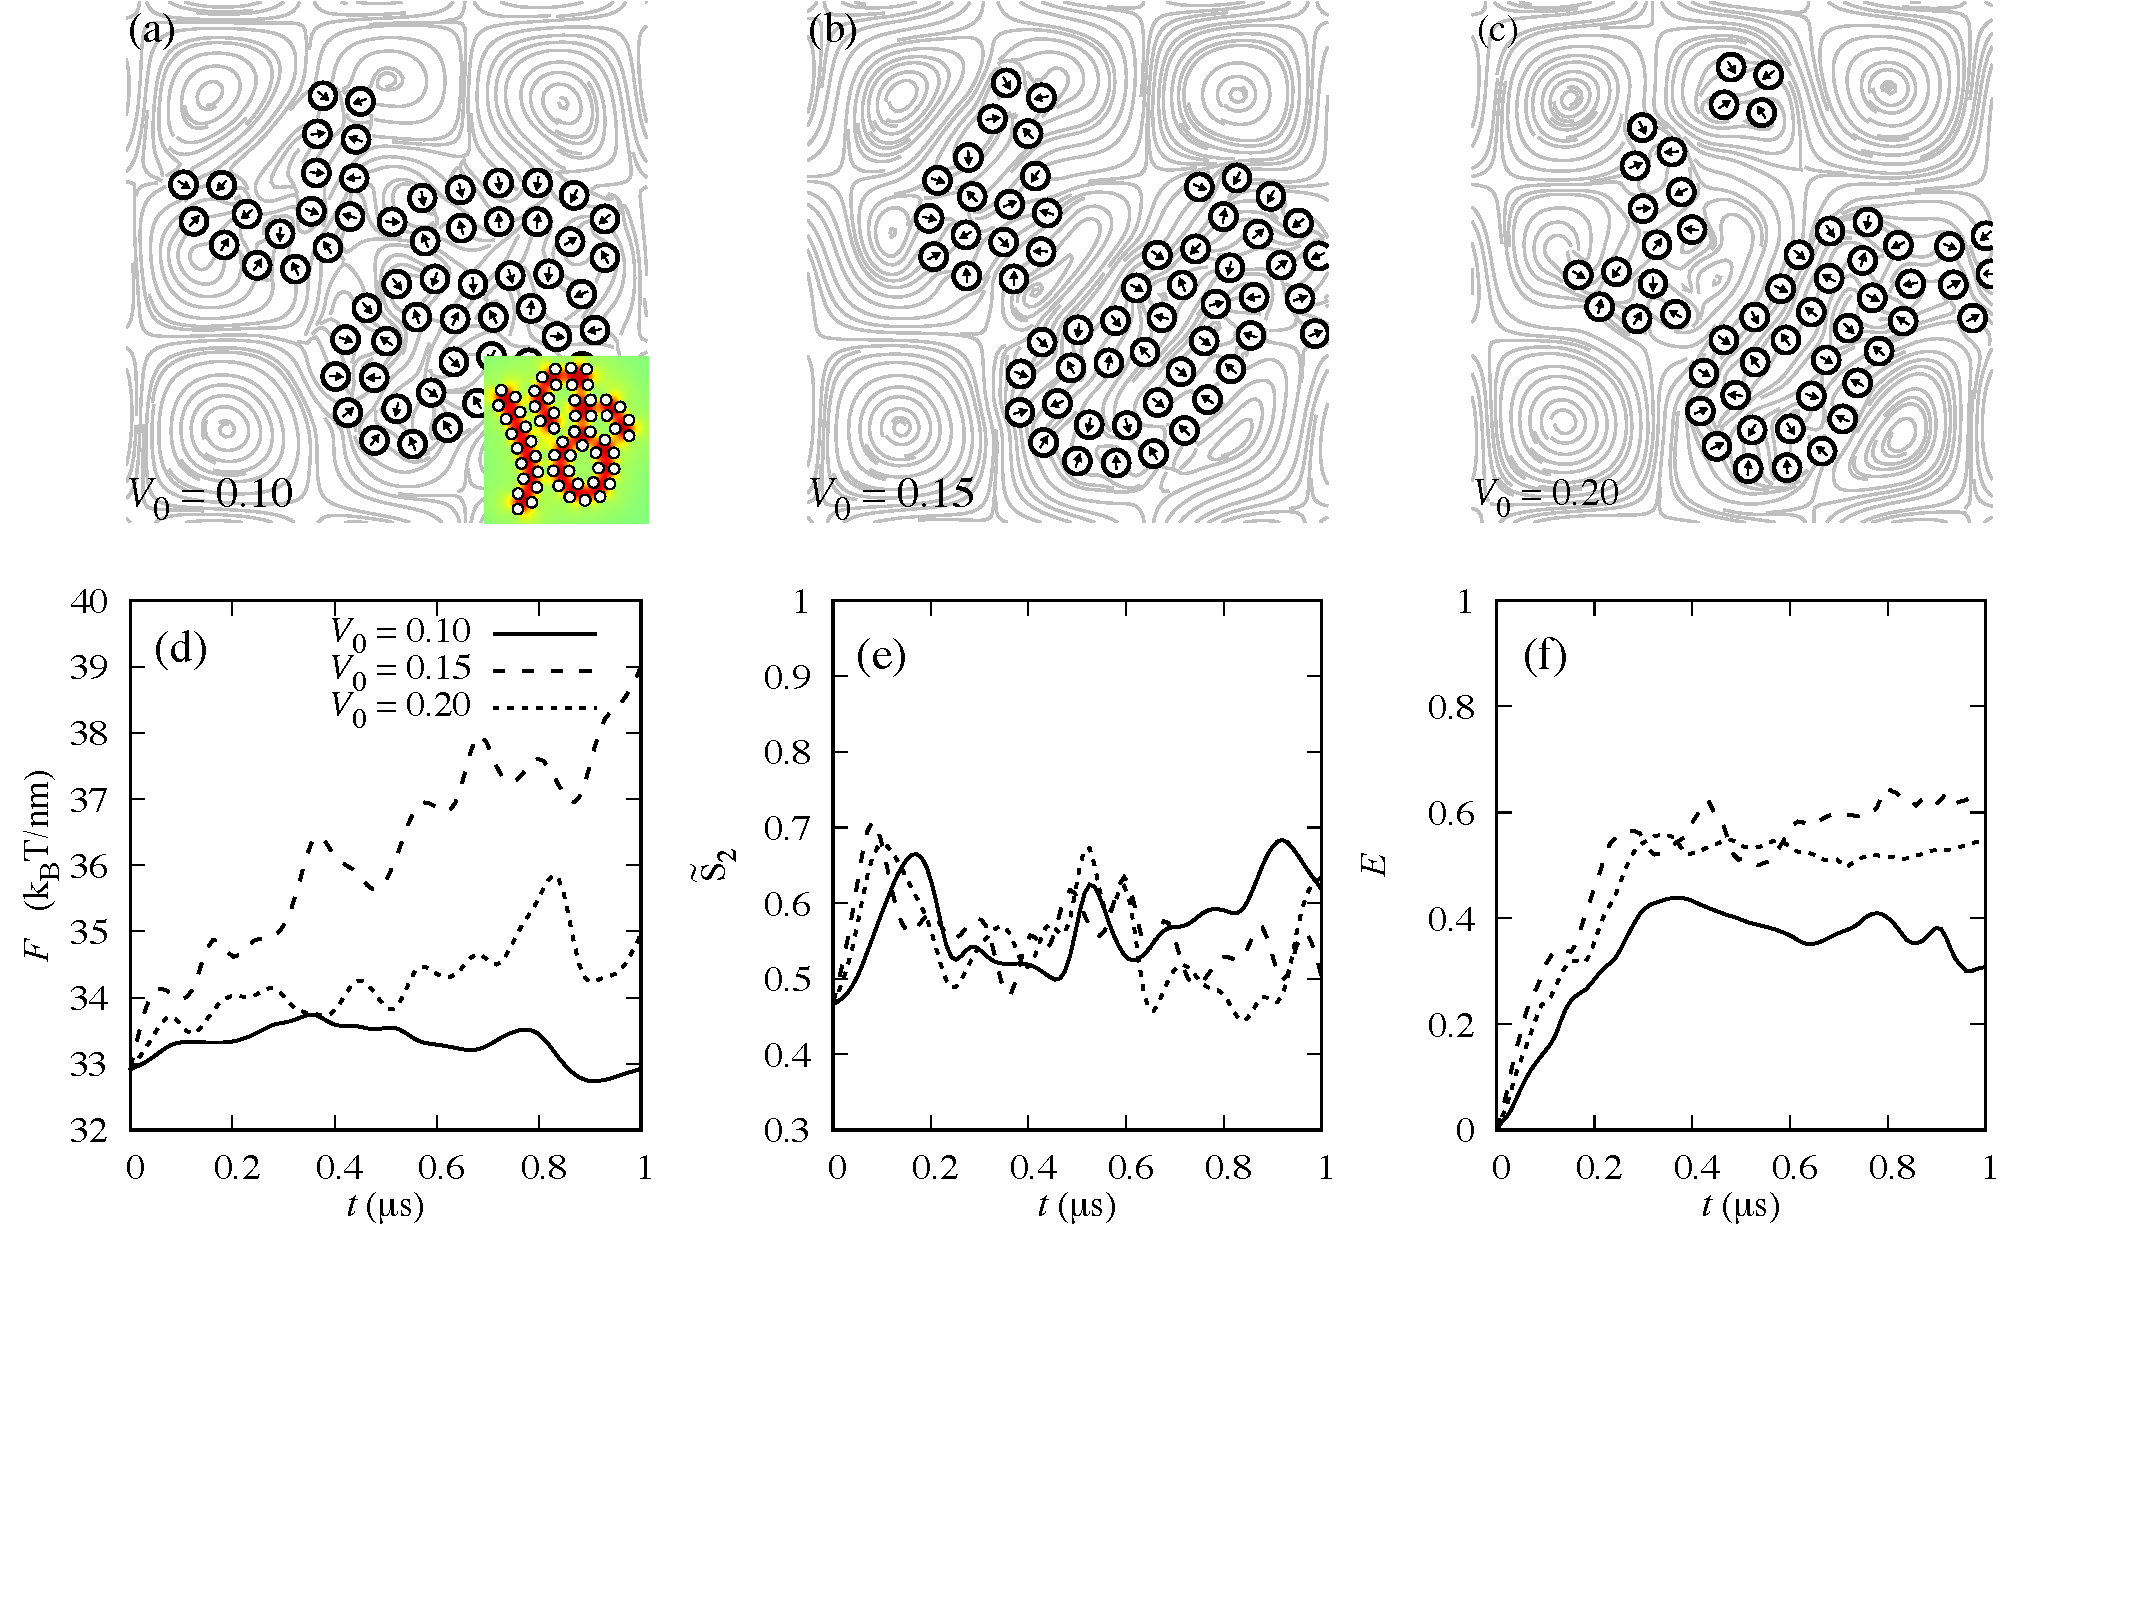
\includegraphics[width=1.0\textwidth]{Figures/Figure5.pdf}    
  \end{center}
  \vspace{-20pt}  
  \caption{\label{fig:BC1_TG} Multiple component bilayers in a
  Taylor-Green when $V_0 = \{0.1, 0.15, 0.2\}$ at $t=0.2\ \upmu$s. The
  pre-relaxed initial configuration is shown in the inset of panel (a).
  The streamlines are plotted in the background. Panel (d) shows the
  free energies; panel (e) shows the orientational parameter
  $\tilde{S}_2$; panel (f) shows the positional parameter $E$.}
\end{figure}
%
\subsection{Bilayer and vesicle configurations in a Taylor-Green flow}
Next, we subject the JP structures to the Taylor-Green (TG) background
flow
\begin{equation}
\label{eq:tg_flow}
\uu_\infty(\xx) = V_0\; \frac{\text{nm}}{\text{ns}}\;
\left(
-\cos\left(x/\lambda\right)
 \sin\left(y/\lambda\right)
         {\bf e}_x
         +\sin\left(x/\lambda\right)
         \cos\left(y/\lambda\right)
             {\bf e}_y\right),
\end{equation}
where $x = {\bf e}_x \cdot \xx$ and $y = {\bf e}_y \cdot \xx$
are the horizontal and vertical coordinates, respectively. 
The TG flow is a confining flow consisting of a checkerboard pattern
of cells with alternating circulation. We control the flow by the
dimensionless flow strength $V_0$ and the dimensionless cell size $l$
defining $\lambda = l$ nm. For most of the results in this subsection,
we use the parameter $l=2$.
%

\begin{figure}
  \begin{center}
    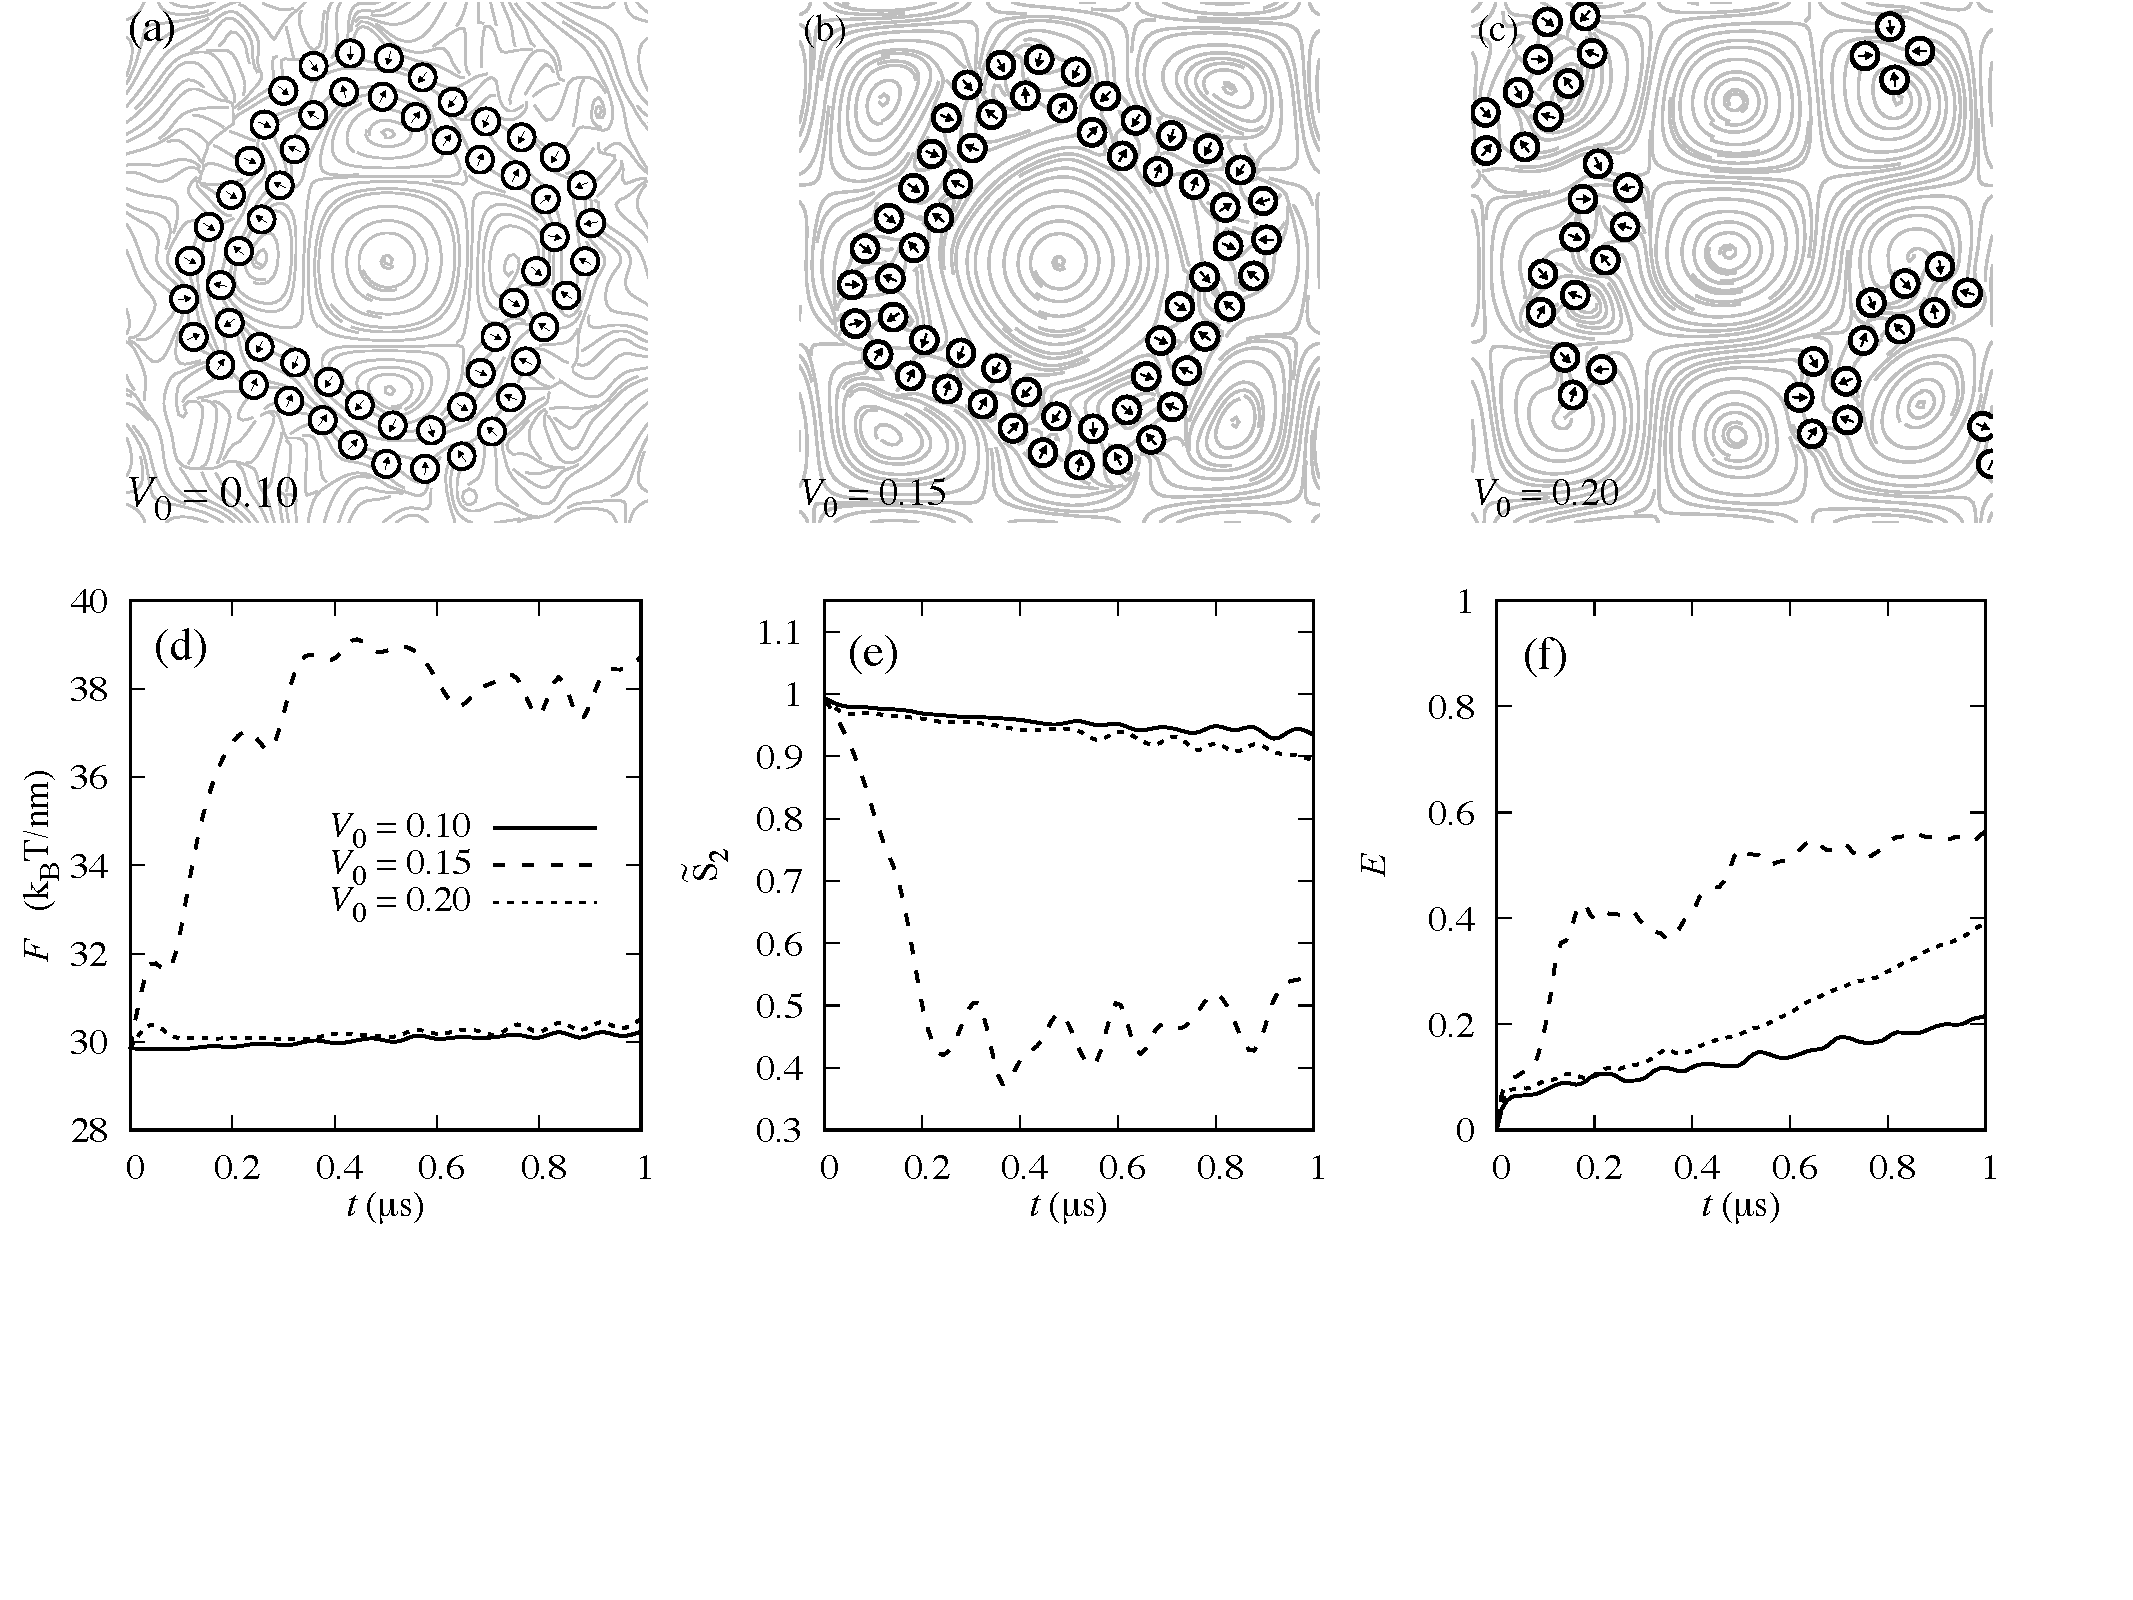
\includegraphics[width=1.0\textwidth]{Figures/Figure6.pdf}        
  \end{center}
\caption{\label{fig:ves_TG} A single vesicle in a TG flow. Panels
  (a)-(c) are snapshots for $V_0=\{0.1, 0.15, 0.2\}$ at $t=0.6\ \upmu$s
  where the pre-relaxed initial configuration is shown in inset of panel
  (a). The streamlines are plotted in the background. Panel (d) shows
  the free energies; panel (e) shows orientational parameter
  $\tilde{S}_2$; panel (f) shows positional parameter E.}
\end{figure}


There is no appreciable pattern in the deformation for the
multicomponent bilayer case in TG flow
(Supplementary Movie S3, right panel).
Figure~\ref{fig:BC1_TG}(a)--(c)
are the snapshots when $V_0=0.1,0.15,0.2$ at $t = 0.2$ $\upmu$s. At all
flow strengths, the bilayer components are separated and mixed by the
flow in neighboring cells. In the $V_0 = 0.2$ case, the flow breaks off
components consisting of only a few particles, leading an increase in
energy (Figure~\ref{fig:BC1_TG}(d), long dashed curve). There is no
apparente structure to the change in the orientational order. There is an initial
increase in the strain parameter due to component mixing, but the
strains remains bounded since the particles stay confined to the
neighbors of the central cell.


Patterns in the deformation, however, do emerge in the case of a vesicle
in TG flow (Supplementary Movie S3, left panel). For a vesicle in a Taylor-Green flow,
Figure~\ref{fig:ves_TG}(a)--(c) are configurations at $t=0.2\ \upmu$s
where $V_0=0.1,0.15,0.2$. Here, the circular vesicle takes on a steady
square shape for moderate flow rates $V_0 = 0.1$ and $V_0 = 0.15$. In
these cases, there is little change in the vesicle free energy and order
(Figure~\ref{fig:ves_TG}(d)--(f)). The vesicle disintegrates for $V_0 =
0.2$ (Supplementary Movie S5, left panel), leading to a jump in energy, drop in order, and increase in
strain, suggesting that the vesicle has a critical TG flow strength in
the interval $0.15 < V_0 <  0.2$ separating the intact and ruptured
end-states.

\begin{figure}
  \begin{center}
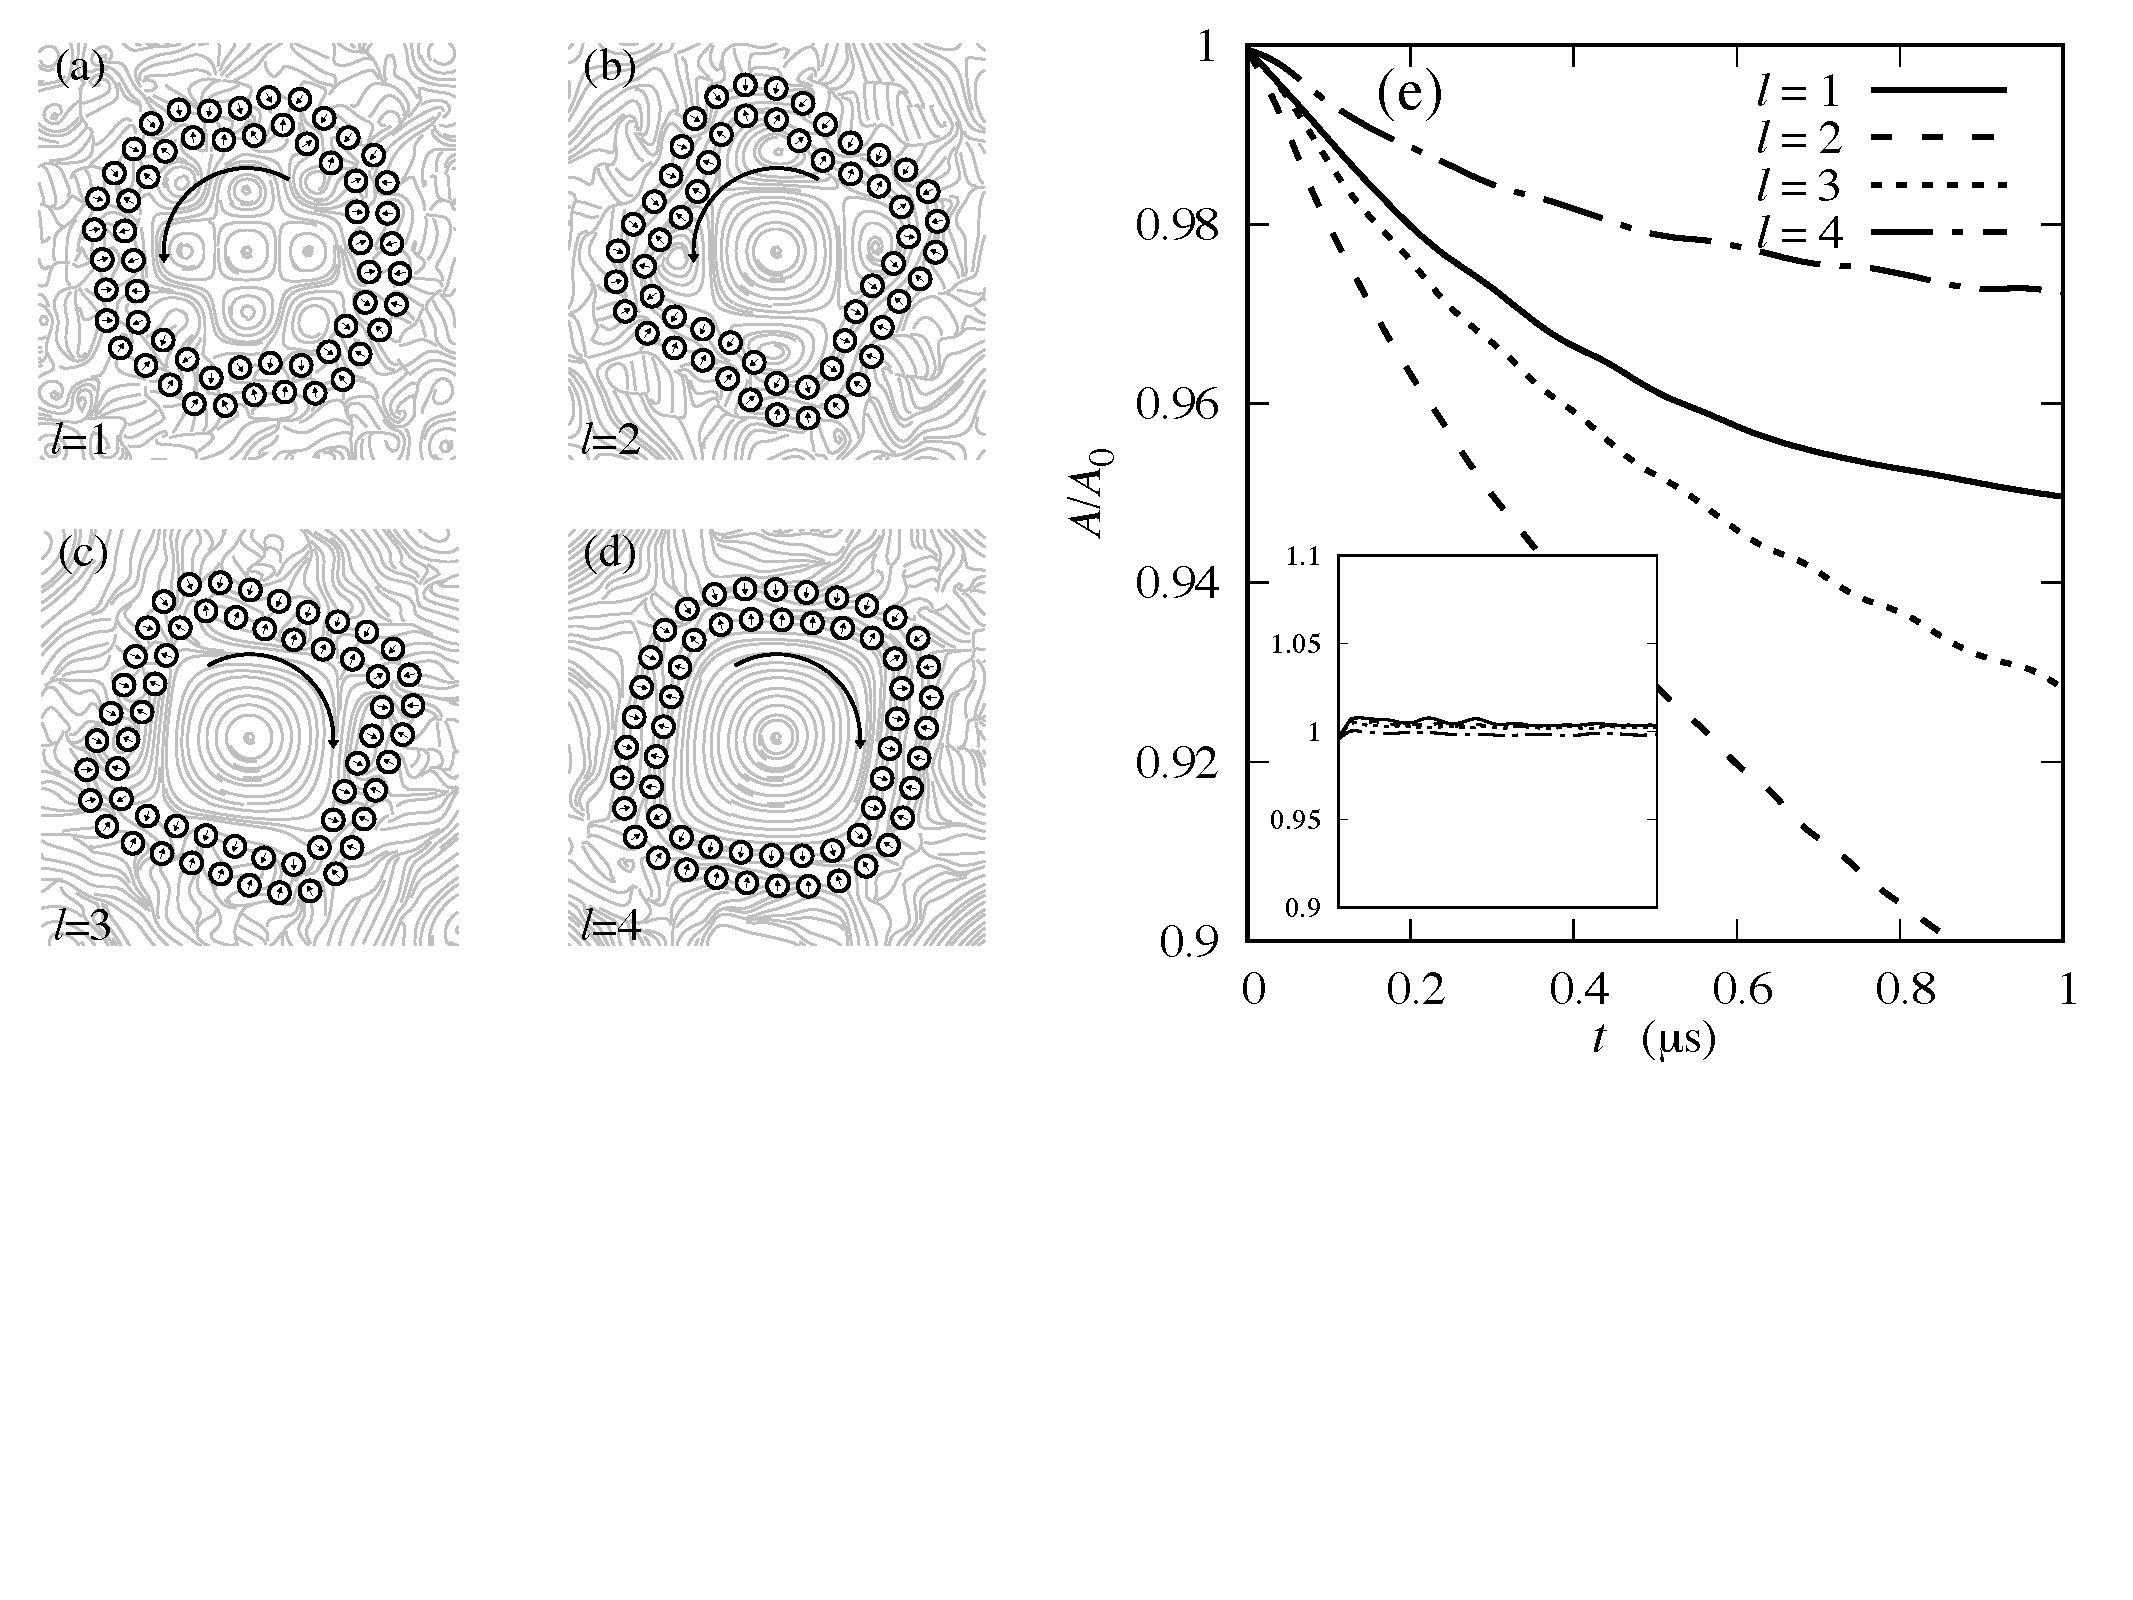
\includegraphics[width=1.0\textwidth]{Figures/Figure7.pdf}
  \end{center}
  \vspace{-20pt}  
  \caption{\label{fig:BTG_Scale} With $V_0=0.1$, panels (a)--(d) show
  the configurations with streamlines of a vesicle is in a TG flow at
  $t=1$ $\upmu$s with $l= 1,2,3,4$, respectively. In panel (e), the
  relative enclosed area $A/A_0$ calculated from the bilayer midplane
  decreases over time. The inset shows the relative length $l/l_0$ which
  remains nearly constant with small magnitude of oscillations. The
  inset and main panel have the same horizontal axis.}
\end{figure}

The vesicle shape is also related to the cell size $l$.
Figure~\ref{fig:BTG_Scale}(a)--(d) show the deformation of a vesicle in
a TG flow for $V_0=0.1$ when $t = 1$ $\upmu$s. For the smallest cell
size $l = 1$ tested, the vesicle is somewhat octagonal and passes
through multiple cells (Figure~\ref{fig:BTG_Scale}(a)). For the largest
cell size $l = 4$, the vesicle is rhomboid and surrounds a single cell. 

In all cases, the vesicle tank-treads like in the shear flow case. The
direction of the tank-treading, however, varies with the cell size
(Figure~\ref{fig:BTG_Scale}(a)--(d), directed arcs). We attribute this
change in rotational orientation to the total rotational moment of the
cells that the vesicle passes through.

We calculate the vesicle area $A$ and length $L$ (initial area $A_0$,
initial length $L_0$) by averaging the area and length of the inner and
outer leaflets. As shown in Figure~\ref{fig:BTG_Scale}(e), the relative
area $A/A_0$ decreases during the simulations, with the rate depending
nonmonotonically on $l$. The relative length $L/L_0$, however, is
constant in $t$ for all cell sizes (Figure~\ref{fig:BTG_Scale}(e),
inset). This implies that the vesicle behaves as an inextensible,
permeable membrane. In previous work, \citet{Fu2022_JFM} determined the
permeability constant of particle-based vesicles in the context of shear
background flow~\cite{chabanon2017, qua-gan-you2021}.



%%%
\begin{figure}
  \begin{center}
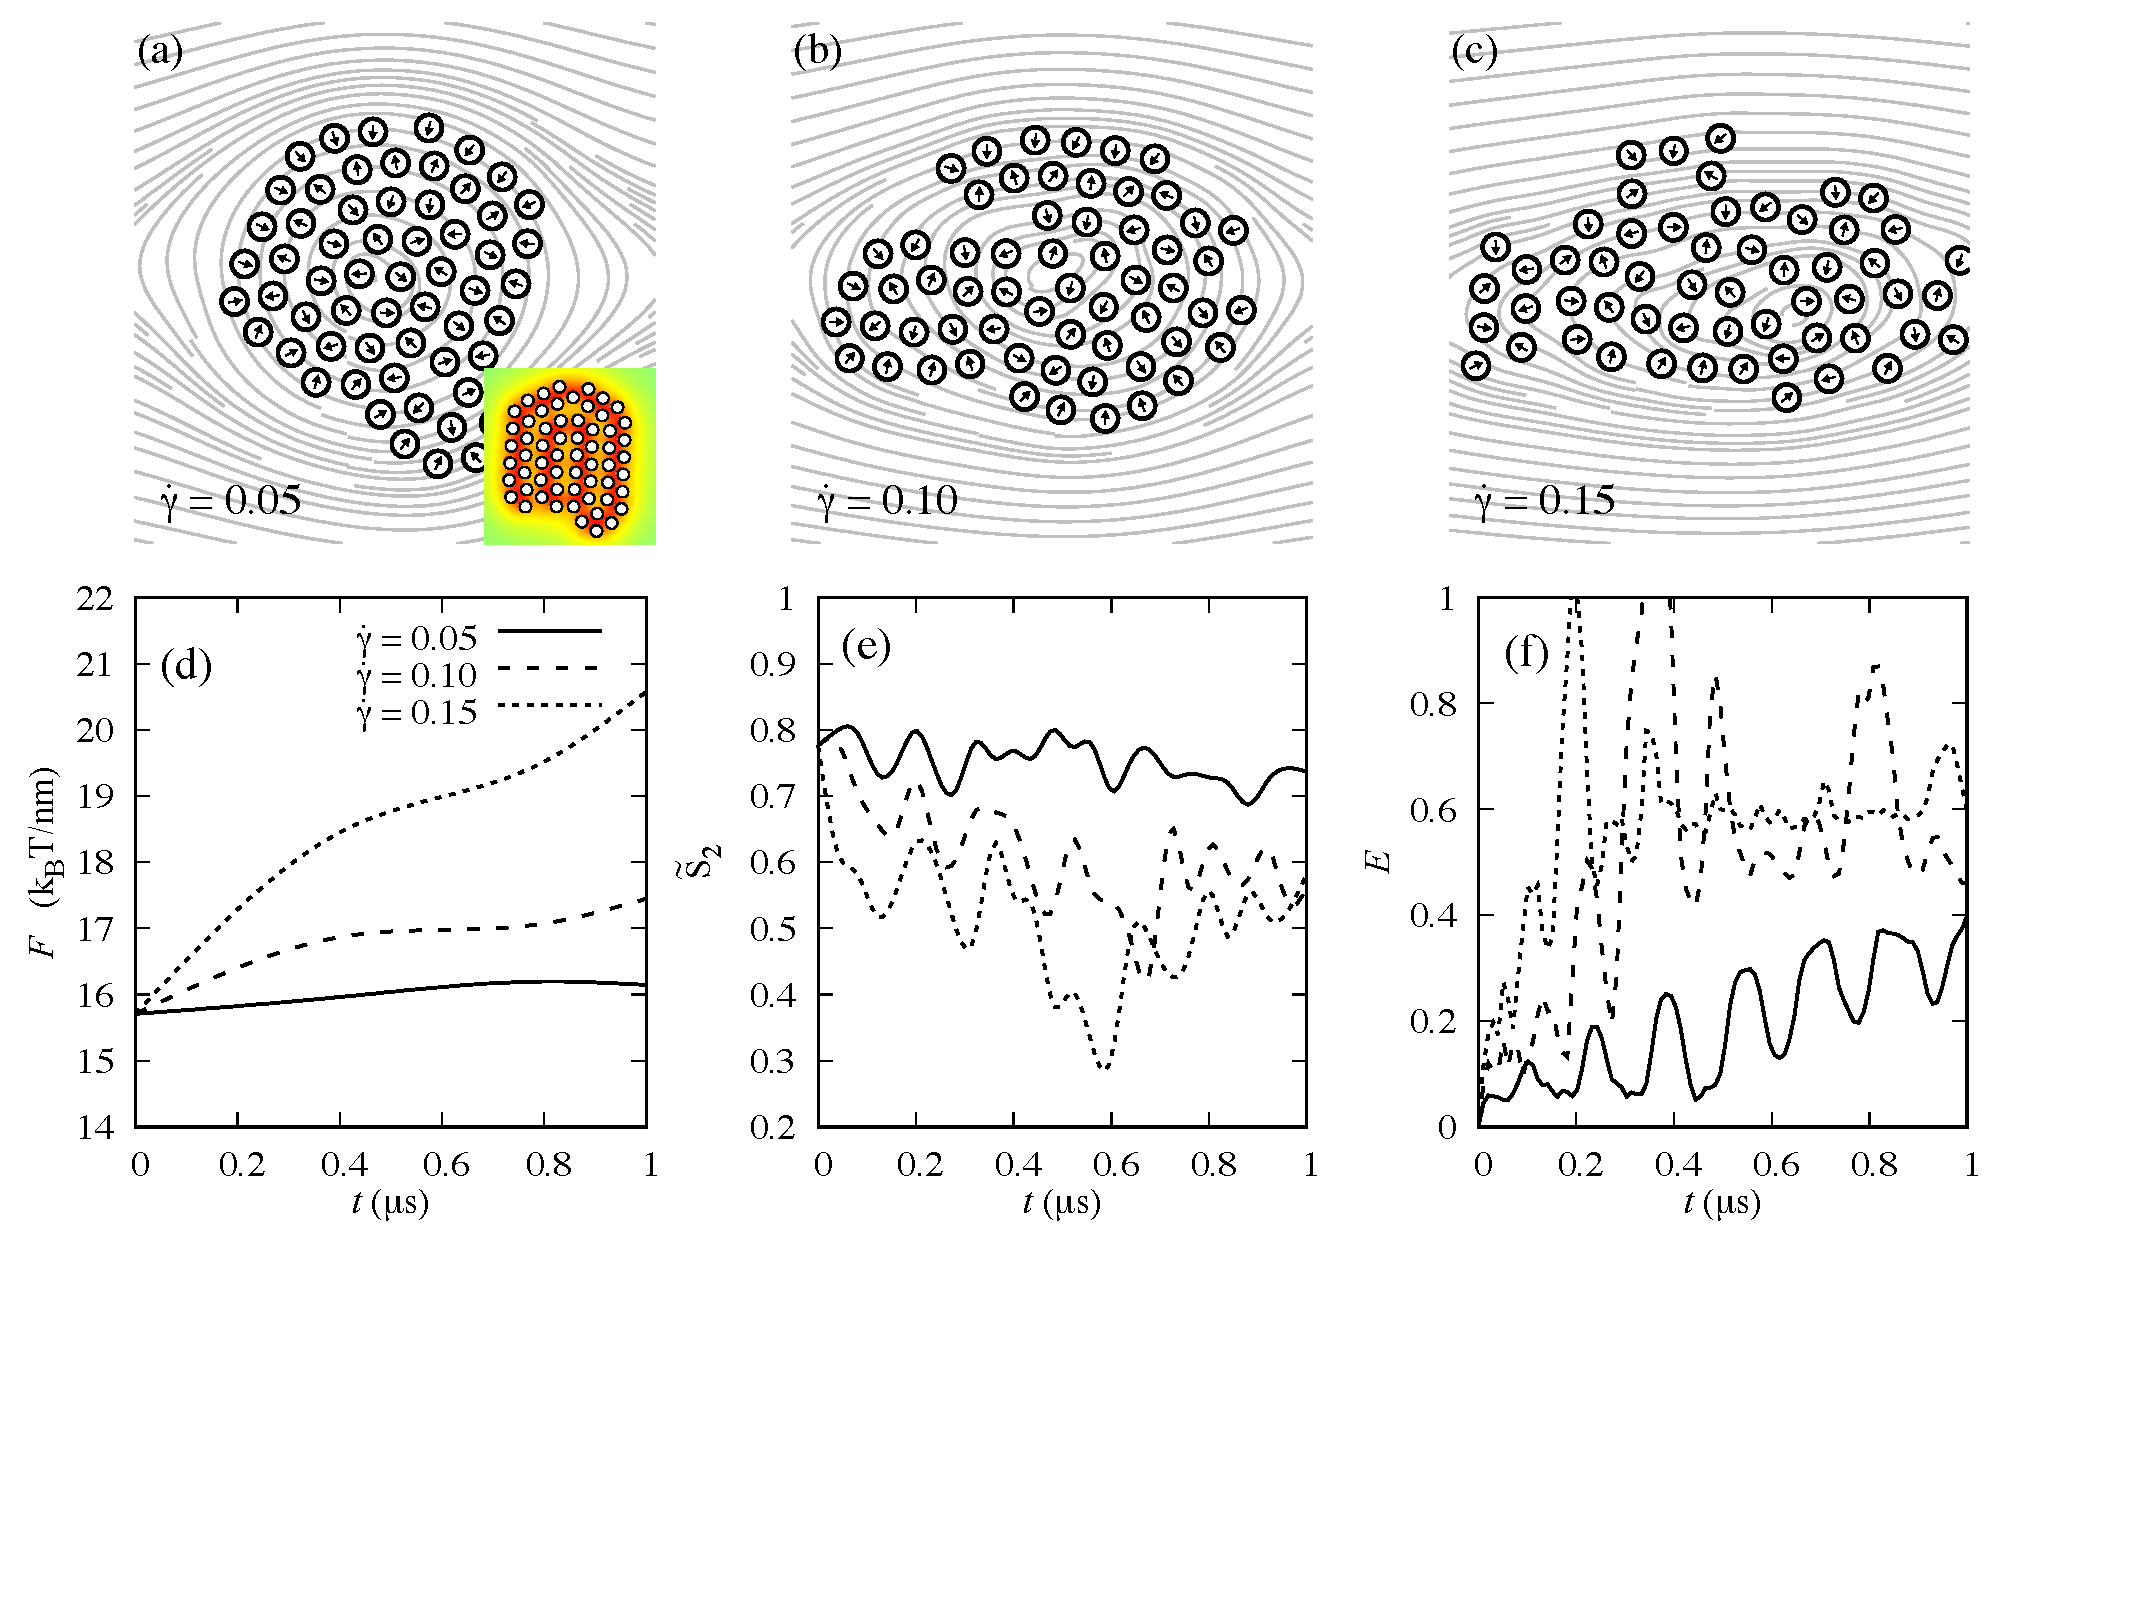
\includegraphics[width=1.0\textwidth]{Figures/Figure8.pdf}
  \end{center}
  \vspace{-20pt}  
  \caption{\label{fig:BC2_shear} A multilamellar structure in a shear
  flow. Panels (a)--(c) are snapshots for $\dot \gamma = \{0.05, 0.1,
  0.15\}$ at $t=0.6\ \upmu$s where the pre-relaxed initial configuration
  is shown in inset of panel (a). The streamlines are plotted in the
  background. Panel (d) shows the free energies; panel (e) shows
  orientational parameter $\tilde{S}_2$; panel (f) shows positional
  parameter E.}
\end{figure}



\subsection{Multilamellar and striated configurations in shear and TG flow}
We have simulated particles for the multilamellar (BC (ii)) and striated
(BC (iii)) boundary conditions, in both shear and TG background flow.
The results are qualitatively similar and will be presented in tandem.
For the multilamellar case, we place a 60-particle configuration (inset
of Figure~\ref{fig:BC2_shear}(a)) in shear flows with $\dot\gamma=0.05,
0.1, 0.15$ and in TG flow with flow rates $V_0=0.1, 0.15, 0.2$. For the
striated case, we also place a 60-particle configuration (inset of
Figure~\ref{fig:BC3_shear}(a)) in shear and TG background flows. Here,
somewhat larger rates are required to see appreciable deformations for
this boundary condition: $\dot\gamma=0.1, 0.125, 0.15$ and $V_0=0.2,
0.25, 0.3$, respectively.
The BC (ii) and BC (iii) in shear flow cases are visualized in
the latter half of 
Supplementary Movie S2 (low shear rate) and 
Supplementary Movie S4 (high shear rate), respectively.
The low and high flow rates for TG flow are shown in
the latter half of
Supplementary Movie S3 and 
Supplementary Movie S5, respectively. 


In terms of shear flow, the free energies are steady at the lowest shear
rates (Figure~\ref{fig:BC2_shear}(d), Figure~\ref{fig:BC3_shear}(d)).
The free energy of the striated configuration oscillates by $\pm 1$
$\mathrm{k_BT}$/nm due to a square reference region deforming into a
rhomboidal shape under shear flow (Figure~\ref{fig:BC3_shear}(d), solid
curve). No such oscillation is present for the multilamellar
configuration since this shape is circularly isotropic
(Figure~\ref{fig:BC2_shear}(d), solid curve). At the lowest shear rates,
there is, however, oscillation in the strains of both configurations,
while the order parameter $\tilde S_2$ is nearly constant
(Figure~\ref{fig:BC2_shear}(e),(f), Figure~\ref{fig:BC3_shear}(e),(f),
solid curves). In summary, both multilamellar and striated
configurations behave as nearly rigid bodies under shear flow when the
shear rate $\dot \gamma$ is low.

In the high shear rate cases ($\dot\gamma=0.15$), both the multilamellar
and striated configurations become disordered. For BC (ii), the lamella
break apart so that individual bilayers are no longer discernible
(Figure~\ref{fig:BC2_shear}(c)). For BC (iii), the stria peel away from
the main body, but remain individually intact
(Figure~\ref{fig:BC3_shear}(c)). Overall, the particles in BC (ii) and
BC (iii) remain bounded and do not drift away in the shear background
flow like for the BC (i) (Figure~\ref{fig:BC1_shear}(c),
Figure~\ref{fig:Ves_shear}(c)).


\begin{figure}
  \begin{center}
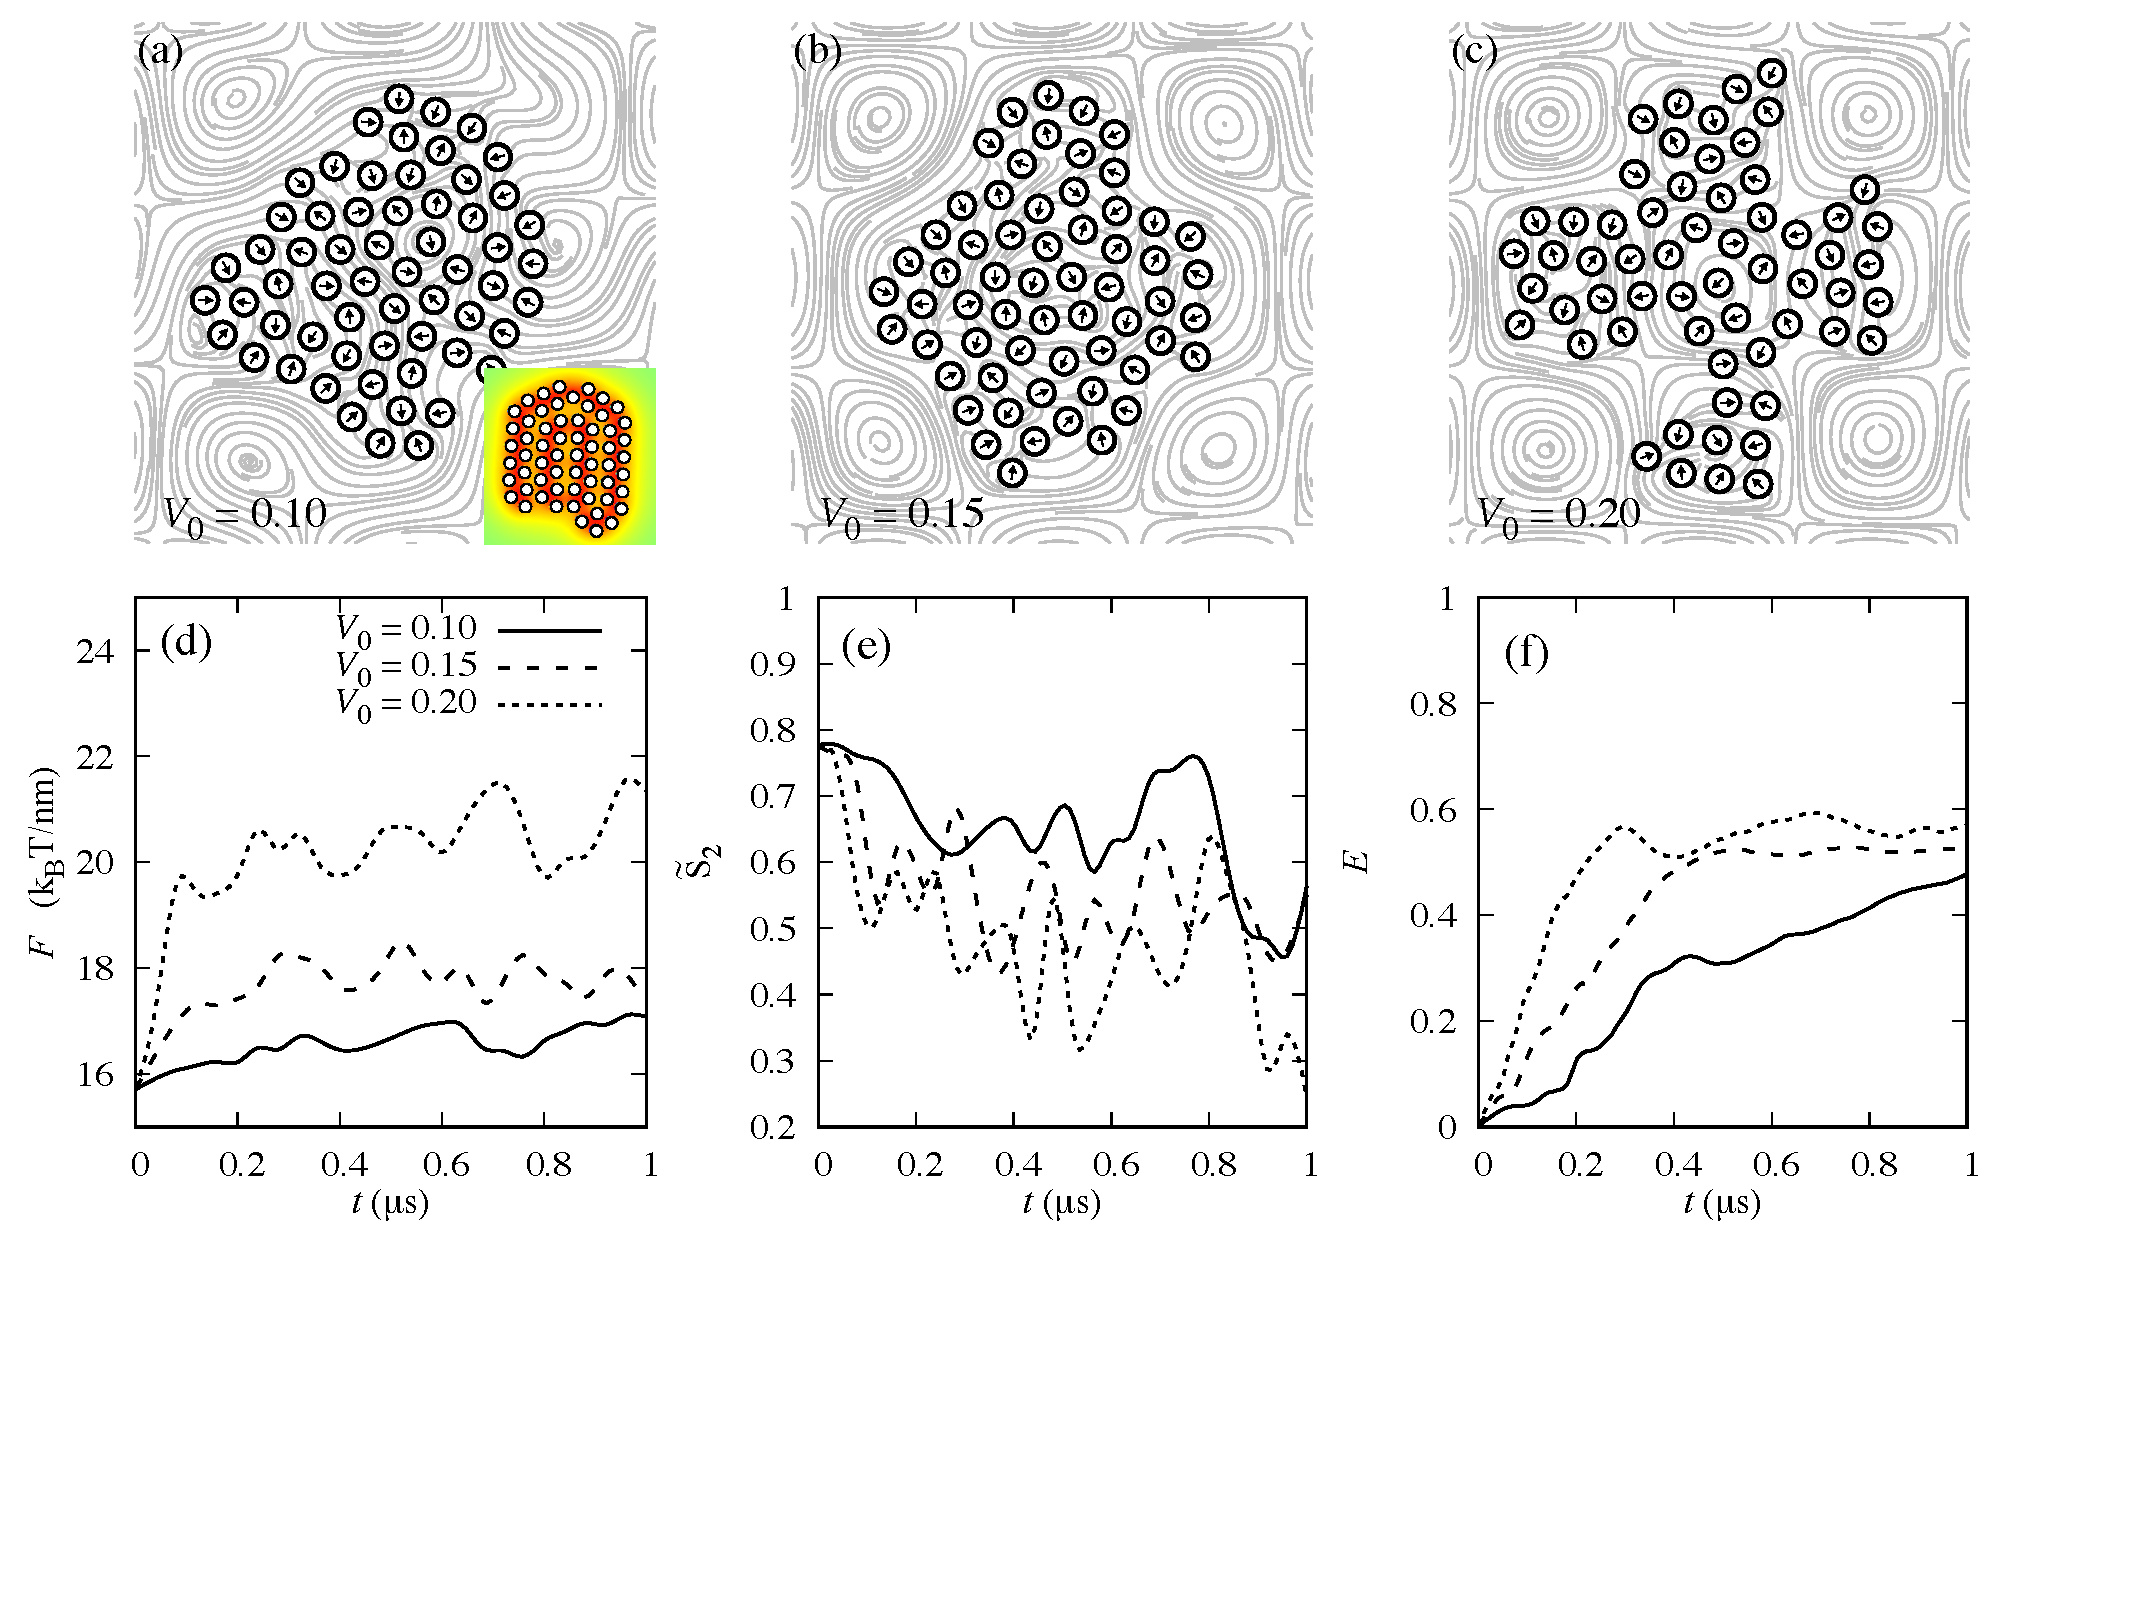
\includegraphics[width=1.0\textwidth]{Figures/Figure9.pdf} 
  \end{center}
  \vspace{-20pt}
  \caption{\label{fig:BC2_TG} A multilamellar structure in a
  Taylor-Green flow. Panels (a)-(c) are snapshots for $V_0 = \{0.1,
  0.15, 0.2\}$ at $t=0.6\ \mu$s where the pre-relaxed initial
  configuration is shown in inset of panel (a). The streamlines are
  plotted in the background. Panel (d) shows the free energies; panel
  (e) shows orientational parameter $\tilde{S}_2$; panel (f) shows
  positional parameter E.}
\end{figure}


Under a TG background flow, the free energy $F$ is also basically
constant for the lowest flow rates $V_0$ (Figure~\ref{fig:BC2_TG}(d),
Figure~\ref{fig:BC3_TG}(d), solid curves). The striated configuration is
unperturbed by the flow, and is engulfed by a single, larger, rotating
flow cell (Figure~\ref{fig:BC3_TG}(a)). The multilamellar configuration
is perturbed by the flow, as seen in the increase in the strain
parameter $E$ (Figure~\ref{fig:BC3_TG}(f), solid curve). The difference
in response to the background flow suggests that the multilamellar
configuration allows for local rearrangement of the particles while
retaining the overall shape.

At large flow rates $V_0$, both configurations depart significantly from
their local equilibrium. The lamella bilayers from BC (ii) break apart,
forming several unlayered bilayer components
(Figure~\ref{fig:BC2_TG}(c)). In BC (iii), the stria also break apart,
but neighboring particles form 'X'-like arrangements
(Figure~\ref{fig:BC3_TG}(d)), resembling the doubly alternating director
equilibrium (Figure~\ref{fig:relax}(d), center, top white rectangle).


%%%

\begin{figure}
  \begin{center}
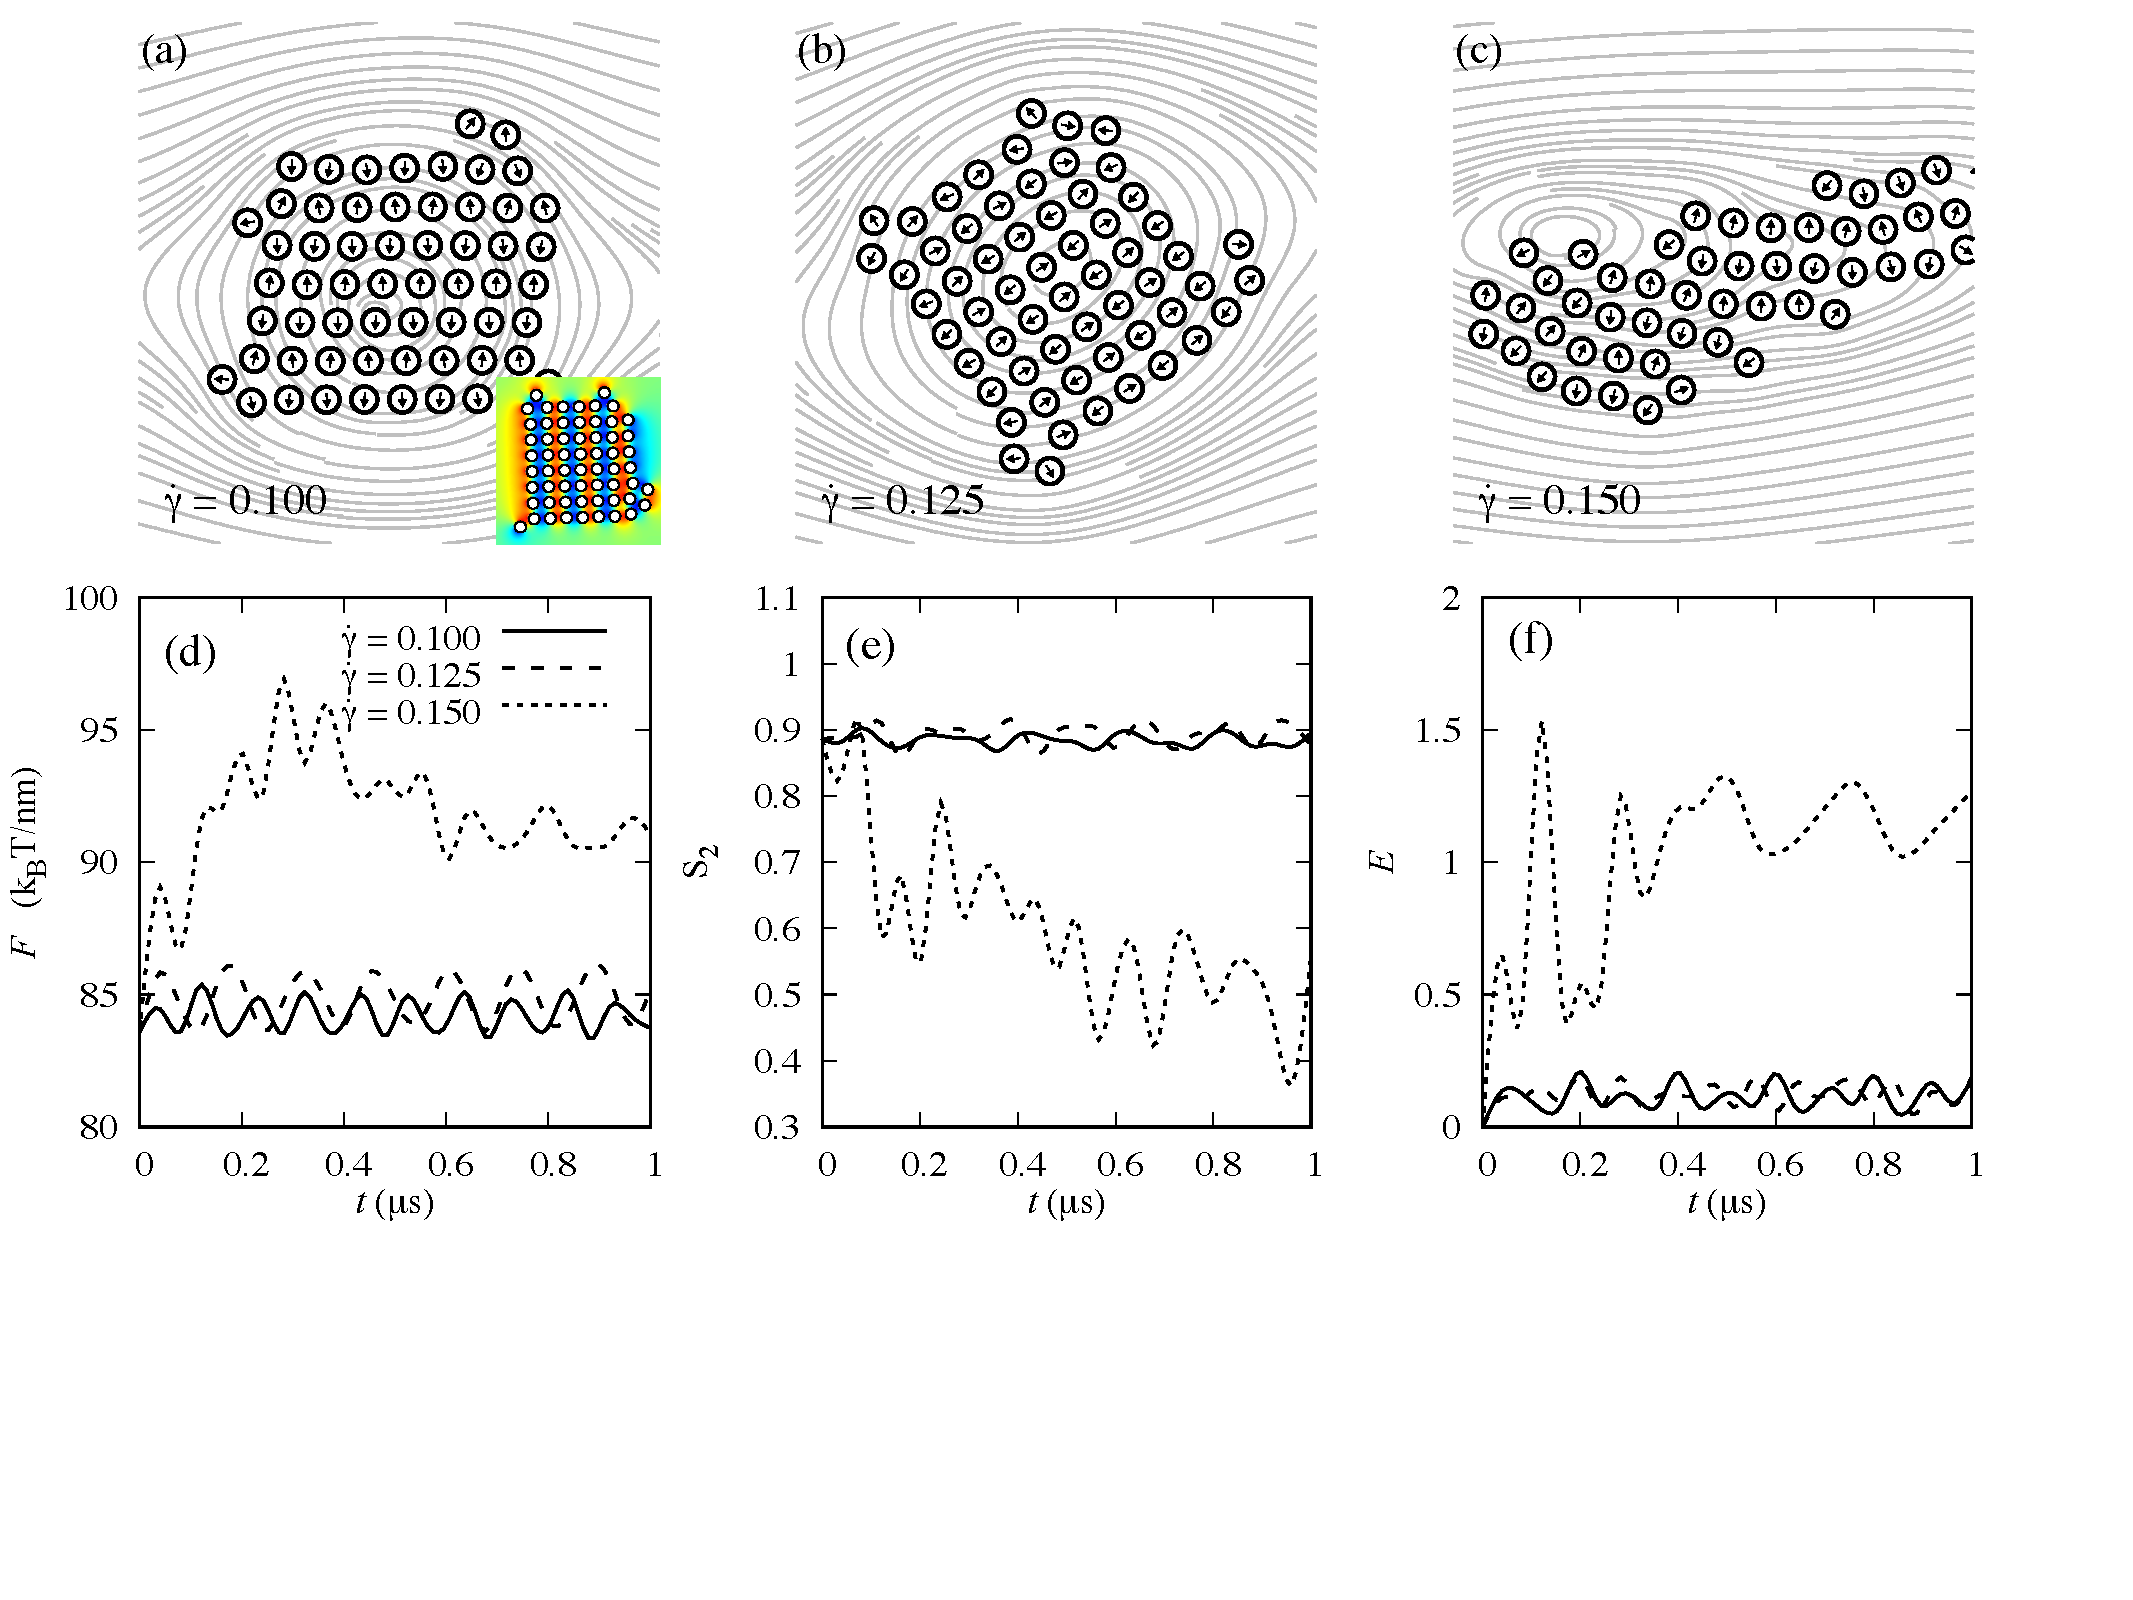
\includegraphics[width=1.0\textwidth]{Figures/Figure10.pdf}        
  \end{center}
  \caption{\label{fig:BC3_shear} A striated configuration in a shear
  flow. Panels (a)-(c) are snapshots for $\dot \gamma = \{0.1, 0.125,
  0.15\}$ at $t=0.1\mu$s where the pre-relaxed initial configuration is
  shown in inset of panel (a). The streamlines are plotted in the
  background. Panel (d) shows the free energies; panel (e) shows
  orientational parameter $\tilde{S}_2$; panel (f) shows positional
  parameter E.}
\end{figure}


\begin{figure}
  \begin{center}
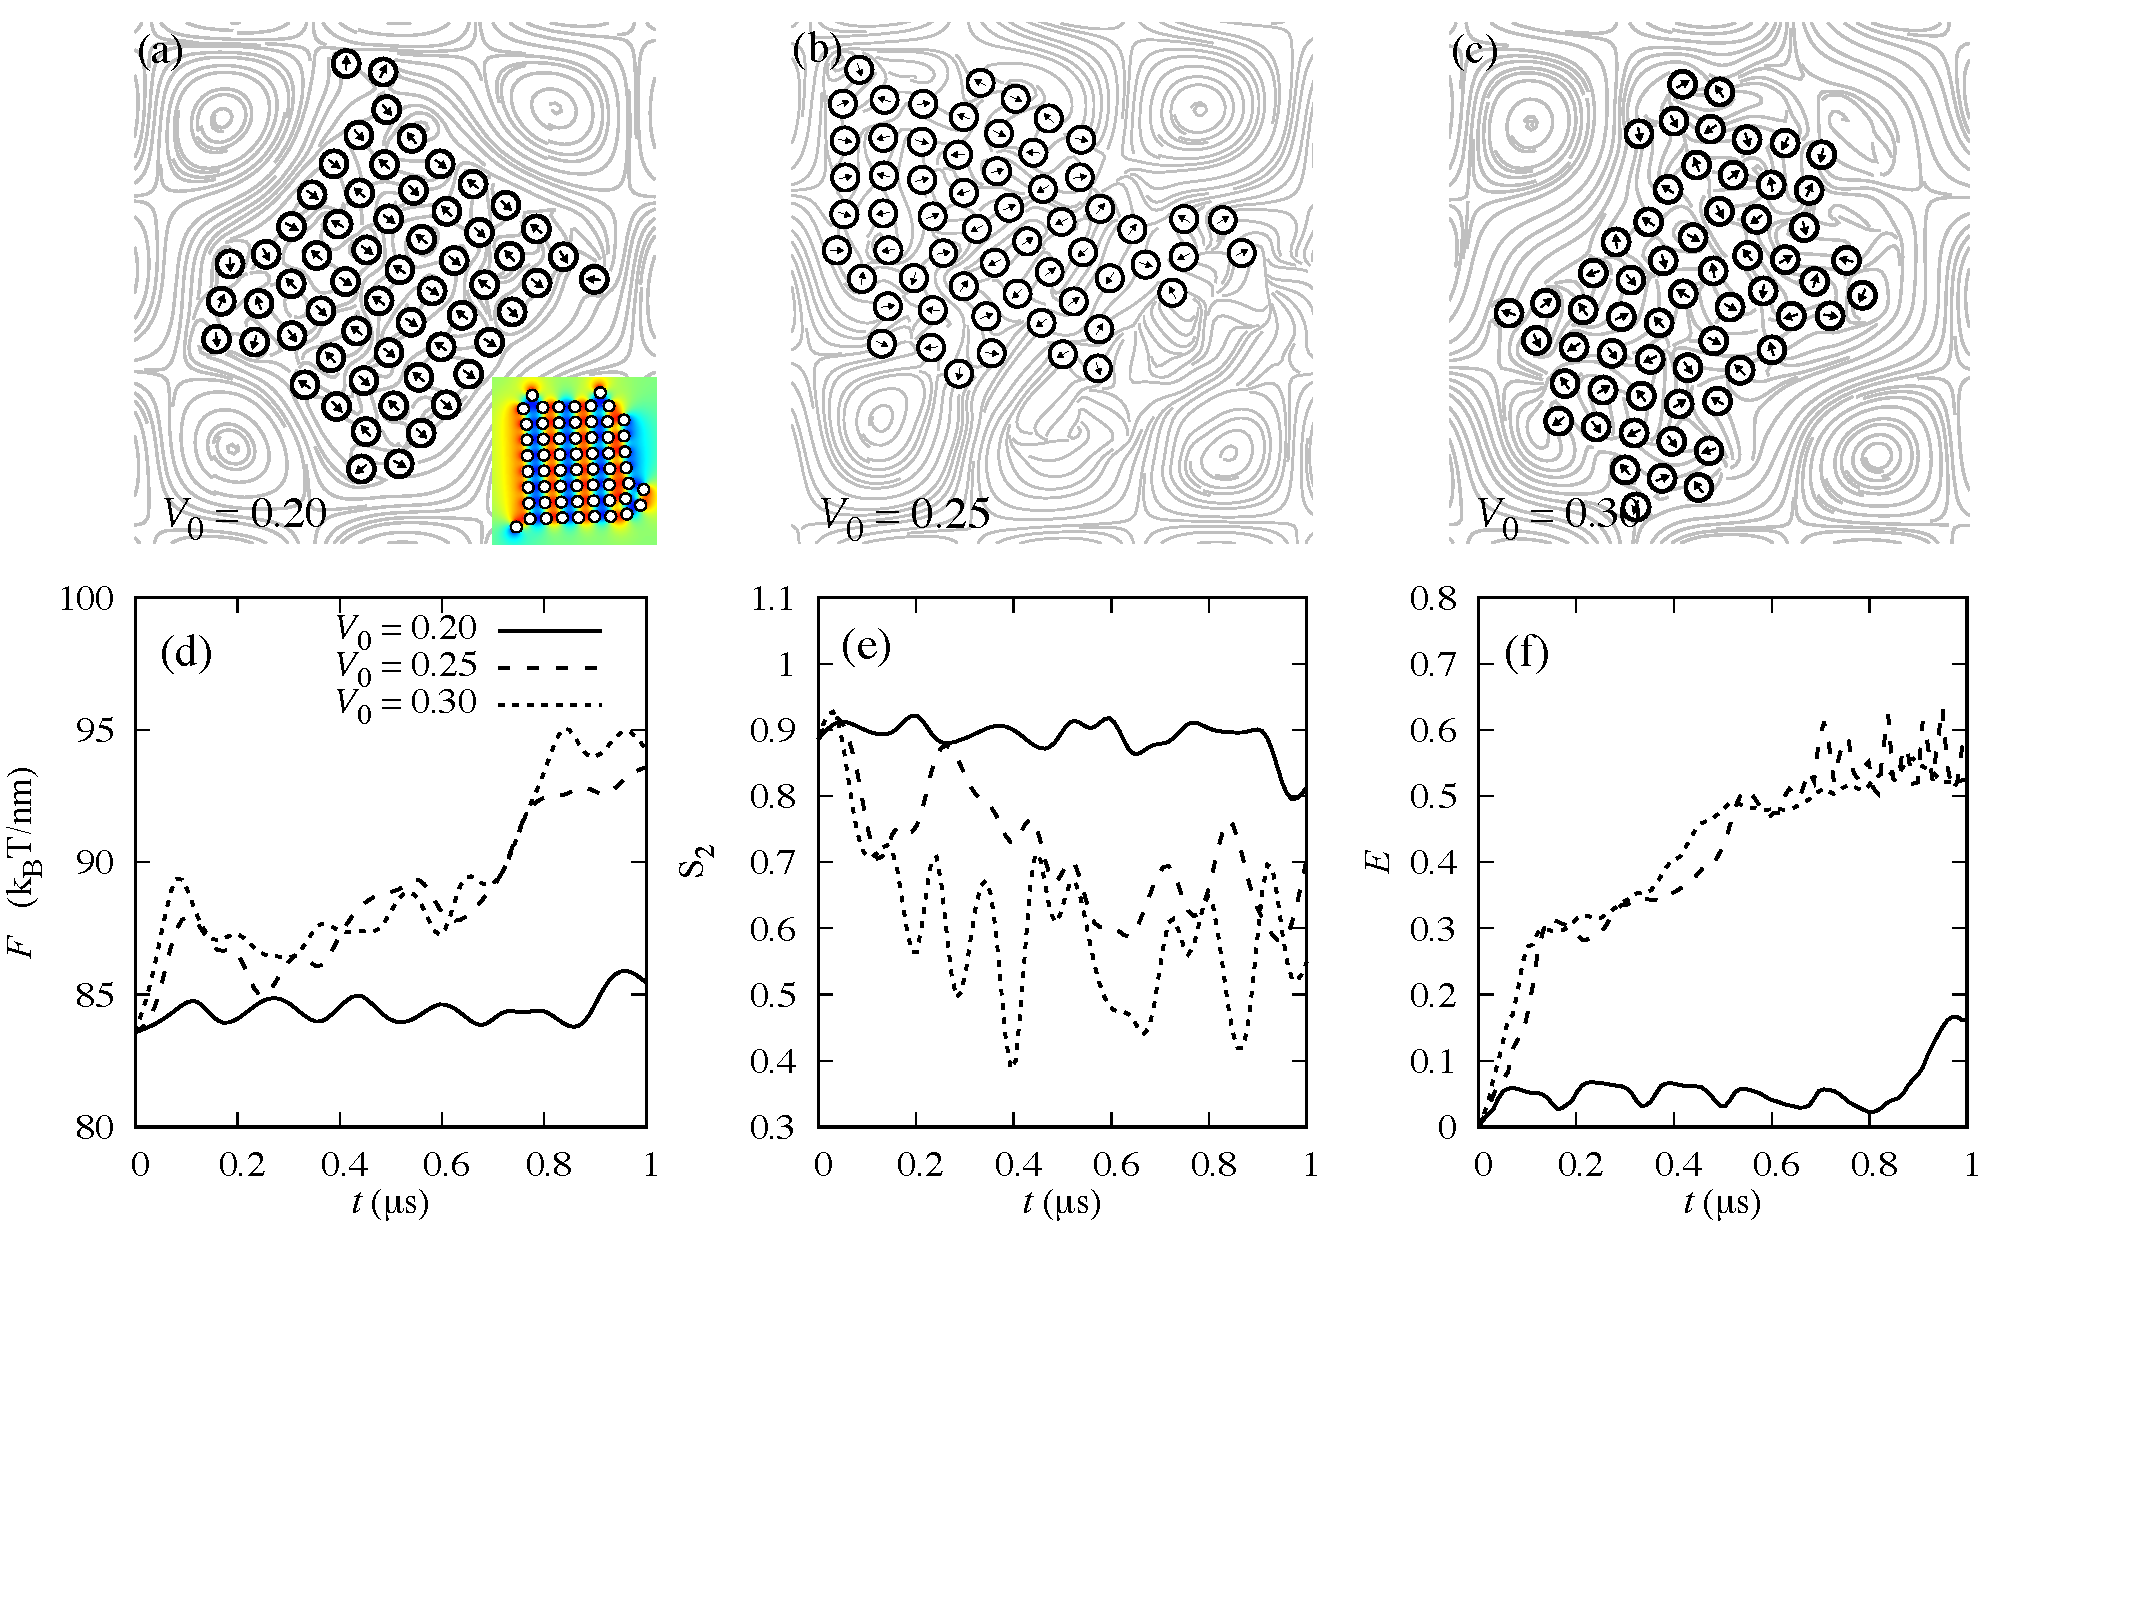
\includegraphics[width=1.0\textwidth]{Figures/Figure11.pdf}            
  \end{center}
  \vspace{-20pt}  
  \caption{\label{fig:BC3_TG} A striated configuration in a Taylor-Green
  flow. Panels (a)-(c) are snapshots for $V_0=\{0.2, 0.25, 0.3\}$ at
  $t=0.4\mu$s where the pre-relaxed initial configuration is shown in
  inset of panel (a). The streamlines are plotted in the background.
  Panel (d) shows the free energies; panel (e) shows orientational
  parameter $\tilde{S}_2$; panel (f) shows positional parameter E.}
\end{figure}



\section{Discussion}
Our results were for $N_b = 60$ particles. This particle number was
large enough for the JP to form measurable structures while giving
manageable simulation times (days) on a single computing processor. The
simulation time for $N_b = 198$ in Figure~\ref{fig:relax} and
Figure~\ref{fig:relax_energy} was several weeks, and so we avoided
simulations of this size for our results. We used $N = 16$ grid points
per particle for all simulations. We performed a convergence study and
found that using $N = 16$ or $N = 24$ grid points per particle gave
quantitatively indistinguishable results. The time courses consisted of
$O(10^3)$ time steps with $\Delta t = 0.2$ nm.

The free energy $F$ defined in~\eqref{eq:free_energy} scales with the
boundary data $g$ and repulsion modulus $M$. To remove the degree of
freedom in the boundary data, we scaled all boundary data so that the
square integral of $g$ is independent of the type of boundary condition; BC
(i), (ii), or (iii). This way, for a fixed configuration, the
hydrophobic interaction portion of the free energy (the integral
in~\eqref{eq:free_energy}) converges to $\gamma N_b$ in the limit
$\rho = 0$. This gives a free energy per particle that is independent of
the shape and intensity of the hydrophobic interface. In practice, $\rho
> 0$ is fixed and the JPs assume different configurations. As a result,
the equilibrium energies per particle in our simulations are different
and depend on the boundary condition (Figure~\ref{fig:relax_energy}).
They are about 0.26 $\mathrm{k_BT}$/nm for BC (ii), 0.55
$\mathrm{k_BT}$/nm for BC (i), and 1.4 $\mathrm{k_BT}$/nm for BC (iii).

Next, we suspended JPs in viscous background flows and observed
deformations as a function of flow strength. There were three categories
of boundary conditions---BC (i), BC (ii), and BC (iii)---that formed
bilayer, multilamellar, and striated configurations, respectively. For
BC (i), we considered both an unstructured bilayer and a vesicle
bilayer. The background flows were a linear shear flow and a TG flow.

We can characterize the effective material properties of the JP
structures based on the changes in free energy, orientational order, and
strain as a function of flow strength. Generally, $F$ increases, $\tilde
S_2$ decreases, and $E$ increases with increases in both $\dot \gamma$
and $V_0$, as expected. Structurally, the striated JP configuration for
BC (iii) behaved the most like a rigid body over the flow strengths
tested. For this structure, the deformation measures were constant in
time for shear rates $\dot \gamma$ up to $0.15$ and TG flow rate $V_0$
up to $0.25$ (Figure~\ref{fig:BC3_shear} and Figure~\ref{fig:BC3_TG}).
Conversely, a $25\%$--$50 \%$ smaller value for $\dot \gamma$ or $V_0$ was
required to observe nonrigid deformations for the BC (i) and BC (ii)
cases.

In terms of fluid behavior, the multilamellar (BC (ii)) structure
behaves as a shear thinning fluid while the striated structure (BC (iii))
has a finite yield stress. Qualitatively, the strains for BC (ii)
increases gradually with shear rate (Figure~\ref{fig:BC2_shear}(f)). In
contrast, the strains for BC (iii) are constant over a range of flow
strengths and then increase when the flow strengths are large enough to
deform the body (Figure~\ref{fig:BC3_shear}(f)). To quantify this
behavior, we form 
\begin{align}
\mu_{\text{asm}} = \frac{\dot \gamma}{\dot E} \mu 
\end{align}
as an effective dynamic viscosity of the particle assemblies. The
numerator $\dot \gamma \mu$ gives the force per area provided by the
solvent stresses where $\mu = 1$ mPa s is the solvent viscosity. The
strain rate $\dot E$ of the body is the slope of a linear fit to the
strain curves e.g., in Figure~\ref{fig:BC2_shear}(f).

Calculated viscosities of particle assemblies are shown in
Table~\ref{tbl:bcii_visc}. The middle row gives the solid area fraction
$\phi$; the sum of the rigid particle areas divided by the total area of
the solvent and particle region. We observe that for the multilamellar
structure, $\mu_{\text{asm}}$ decreases with increasing shear rate. The
predicted viscosities of the particle assemblies are on the order of
hundreds of times that of water, consistent with suspension viscosities
for noninteracting particles~\cite{KONIJN201461}. In the case of
striated structures, viscosity is effectively infinite for the lower two
of the shear rates, and then drops to a finite value $\mu_{\text{asm}} =
60$ mPa s when the shear rate reaches $0.15$ ns$^{-1}$.
\begin{table}
  \caption{\label{tbl:bcii_visc} The dynamic viscosity of assemblies
  $\mu_{\text{asm}}$ (mPa s).}
\centering
\begin{tabularx}{0.7\textwidth}{c|X|X|X||X|X|X}
&\multicolumn{3}{c||}{BC (ii)} & \multicolumn{3}{c}{BC (iii)}\\
\hline
  $\dot \gamma$ & 0.05 & 0.10 \quad & 0.15 & 0.100 & 0.125 & 0.15\\
  \hline
  $\phi$ & 0.50 & 0.47 & 0.41 & 0.47 & 0.46 & 0.45 \\
  \hline
  $\mu_{\text{sus}} $ & 401 & 66 & 42 & 2.5e3 & 1.4e3 & 60\\
\hline
\end{tabularx}
\end{table}

In the case of BC (i), our previous work~\cite{Fu2022_JFM} calculated a
friction coefficient $b$ for the intermonolayer slip between the two
leaflets of a bilayer. \citet{denOtter2007,Zgorski2019} and
\citet{doi:10.1073/pnas.2100156118} have calculated in-plane viscosities
for fully three-dimensional bilayers. Although not part of this work, it
is in principle possible to obtain an in-plane viscosity using the
hydrophobic potential~\eqref{eq:free_energy} by replacing the boundary
condition~\eqref{eq:bc-type} with one that is everywhere constant, in
effect modeling lipids in a bilayer as an array of elongated, purely
hydrophobic pillars. 

While increased flow strengths generally injected energy into the
suspension, the simulation results show that the unstructured bilayer
actually increases orientational order and has somewhat lower free
energy under low shear rates (Figure~\ref{fig:BC1_shear}(d,f)). This
effect suggests that in amphiphilic suspensions, it might be possible to
decrease the excess area of the system by subjecting the suspension to a
moderate shear flow (Supplementary Movie S2, right panel).
Not all background flows produce this
``organizing'' effect, as it is not observed in the TG background flow
case (Figure~\ref{fig:BC1_TG}, Supplementary Movie S3, right panel).
\citet{PhysRevLett.128.256102} have
shown how to drive particle clusters into arbitrary target shapes by
solving a first passage problem.

The characteristics of the self-assembly of amphiphilic JP into
onion-like dendrimersomes like for BC (ii) were previously studied by molecular dynamics
simulations~\cite{C9NR05885K}. The molecular dynamics simulations use an
anisotropic pair potential to describe the particle interactions
where a harmonic form describes the repulsive part and an anisotropic
attractive part describes the hydrophobic interactions.

\citet{kohl-cor-che-vee22} have simulated JP suspensions in three
dimensions using the same free energy formulation of hydrophobic
attraction used in the present work. They observed spontaneous
aggregation into micelles generically and formation of bilayers when the
initial configuration was chosen sufficiently close to the final
configuration. They also studied self-assembly of bipolar electric JP,
which use BC (ii) but electric potential, instead of a water order parameter,
to define the interaction.  Due to the differing interaction,
bipolar electric particles form parallel chains that
repel. In contrast, the hydrophobic interaction between stria is
attractive. The existence of 'X'-shaped local arrangements as a local
equilibrium (Figure~\ref{fig:relax}(d), top, middle rectangle) further
suggests there may be greater diversity in the set of possible
equilibria in three-dimensions when employing hydrophobic attraction.


\section{Conclusion}
\label{sec:conclusion}


In this work, we employ the newly developed JP model using BIEs ~\cite{Fu20, Fu2022_JFM} 
and tune the boundary conditions with energy normalization to study the dynamics of 
amphiphilic (BC(i)), biased hydrophobic (BC (ii)), and bipolar (BC(iii)) JPs.
To overcome the well-known 
obstacle for numerical implementations in the free energy $F$ where the gradient of 
solution to the screened Laplace equation involves hyper-singularities, we derive the normal 
derivative \eqref{eq:normal_deriv} in terms of single layer potential $\SSS$.

Simulations include the self-assembly behaviors when the flow is absent and
when JP are subject to shear and TG background flows with various 
flow strengths. The free energy profiles demonstrate that the relaxation process for 
particles confined in a certain size of box is independent of number of particles 
($N_b$). However, the final configurations highly depend on the initial particle 
directors $\dd_i$. Therefore, multiple patterns or local energy minimum states may 
appear depending on the initial setup.

We track the total free energy, the orientational order parameter,
and the strain parameter to comprehensively summarize and classify the effective properties
of all three materials. 
Observations have shown that multi-lamella and the striated structures under a relatively 
weak linear shear flow behave like a rigid body with minimal deformation. The effective 
viscosity of the material gives a quantitative validation to support the statement. High 
shear-rate cases provide a range for critical shear rates where the structures break 
apart and undergo major topological changes. As expected in all case studies,
free energy, orientationl order, and strain combined 
are good topological indicators.

Under a TG flow, we examine the same measures and simulate all structures with 
the same criteria as ones in shear flow cases. In addition, for JP vesicle under a 
TG flow, we compare the results when the size of cell is varied and a nonmonotonic 
trend in reduced area with respect to the cell size arises. One finding to be noted is 
that the TG flow with specified parameters can effectively control the structure shapes 
such as a square vesicle or a polygonal shape. 

The results reported here provide an inroad computational framework for colloidal sciences. 
The present study also helps us to understand more rheological properties of industrially 
produced JP.
This study can be extended to three dimensional systems 
and it has been included in our future goals\cite{kohl-cor-che-vee22}.
From a numerical perspective,
it is straightforward to include
random perturbations in the particle shape and
boundary condition that mimick interfacial properties
found in lab conditions\cite{Bradley2016,Bradley2017}.

\section{Appendix}
\label{sec:appendix}
Our calculation of the free energy $F$ relied on 
converting the body integral in \eqref{eq:free_energy}
into the surface
integral in \eqref{eq:free_energy2}
involving only single layer potentials and
tangential derivatives. 
This section supplies a proof of identity
\eqref{eq:normal_deriv} used in this conversion.
Let 
\begin{equation}
  \label{eq:SLP}
  \mathcal{S}[\sigma](\xx) = \int_\Gamma G(\xx-\yy) \sigma(\yy)\, \dif s_\yy
\end{equation}
be the single layer potential for a density function $\sigma.$
Fix $\xx \in \Gamma$,
let $\nnu_{\xx} = \nnu(\xx)$ and $\nnu_{\yy}$ be the unit normal at $\xx$, respectively $\yy$, in $\Gamma$,
and let $\zz \in \Omega$.  The subscripts in $\nabla_{\zz}$ and $\nabla_{\yy}$ denote
differentiation with respect to $\zz$, respectively $\yy$.

Recall from \eqref{eq:SL_BIE} that $u = \mathcal{D}[\sigma]$.
Then  
\begin{align*}
\nabla_{\zz} u(\zz) \cdot \nnu_{\xx}
&=\nnu_\xx \cdot \nabla_\zz \int_\Gamma \frac{\partial G(\zz-\yy)}{\partial \nnu_\yy}\sigma(\yy) \,\dif s_\yy\\
&=\int_\Gamma \nnu_\xx^\top \left(\nabla_\zz\nabla_\yy^\top  G(\zz-\yy)\right) \nnu_\yy\sigma(\yy)  \,\dif s_\yy\\
  &=-\int_\Gamma \nnu_\xx^\top \left(\nabla_\yy\nabla_\yy^\top G(\zz-\yy)\right)\nnu_\yy\sigma(\yy)\ \dif s_\yy,
\end{align*}
since we can interchange $\nabla_\zz$ with $-\nabla_\yy$.
Following \cite{Hsiao2008}, \S 1.2,
\[
\nnu_\xx^\top \left(\nabla_\yy\nabla_\yy^\top G(\zz-\yy)\right)\nnu_\yy
=
-\tt_{\xx}^\top \left(\nabla_\yy\nabla_\yy^\top G(\zz-\yy)\right)\tt_{\yy}
+ \Delta_{\yy}G(\zz-\yy) \tt_{\xx}\cdot \tt_{\yy}.
\]
Then, using that $\Delta_{\yy} G(\zz-\yy) = \rho^{-2} G(\zz-\yy)$,
interchanging $\nabla_\yy$ with $-\nabla_\zz$ once more,
and integrating by parts in arclength $s$,
we obtain 
\begin{align*}
\nabla_{\zz} u(\zz) \cdot \nnu_{\xx}
&=-\int_\Gamma  \Delta_\yy G(\zz-\yy) {\bf t}_\xx \cdot   {\bf t}_\yy \sigma(\yy)\ \dif s_\yy
+\int_\Gamma({\bf t}_\xx\cdot\nabla_\yy)({\bf t}_\yy\cdot\nabla_\yy G(\zz-\yy))\sigma(\yy)\ \dif s_\yy\\
&= -\int_\Gamma \frac{1}{\rho^{2}} G(\zz-\yy) {\bf t}_\xx \cdot {\bf t}_\yy \sigma(\yy)\ \dif s_\yy  
-({\bf t}_\xx\cdot\nabla_\zz)\int_\Gamma \frac{\dif}{\dif s_\yy}G(\zz-\yy) \sigma(\yy)\ \dif s_\yy\\
&= -\frac{1}{\rho^2} {\bf t}_\xx\cdot \int_\Gamma G(\zz-\yy){\bf t}_\yy \sigma(\yy)\ \dif s_\yy + 
({\bf t}_\xx \cdot \nabla_\zz)\int_\Gamma G(\zz-\yy)\frac{\dif }{\dif s} \sigma(\yy)  \dif s_\yy.
\end{align*}
%
Letting $\zz\to\xx\in\Gamma$, and noting that both sides of the equation are continuous,
we obtain \eqref{eq:normal_deriv}.


% If you have acknowledgments, this puts in the proper section head.
\begin{acknowledgments}
We thank Dr.~S\'ebastien Michelin and Dr.~Cecile Cottin-Bizzonne from LadHyX - Ecole Polytechnique Institut Polytechnique de Paris for organizing the focus-session ``interfacial active matter'' in the conference APS-DFD 2021 and the invitation of submitting a special collection paper. 

% put your acknowledgments here.
\end{acknowledgments}

% Create the reference section using BibTeX:
\bibliography{reference}


\thispagestyle{empty}

\newpage
{\Large \bf

  \noindent Supplementary Material\\

  \noindent 
 Effects of Tunable Hydrophobicity on the Collective Hydrodynamics of Janus Particles under Flows}\\

\noindent 
Szu-Pei Fu$^{1,*},$ 
Rolf Ryham$^{2},$ 
Bryan Quaife$^{3}$ and Y.-N. Young$^{4},$
\\

\noindent
$^{1}$Department of Mathematics, Trinity College, Hartford, Connecticut 06106, USA

\noindent
$^{2}$Department of Mathematics, Fordham University, Bronx, NY, USA

\noindent
$^{3}$Department of Scientific Computing, Florida State University, Tallahassee, Florida 32306, USA

\noindent
$^{4}$Department of Mathematical Sciences, New Jersey Institute of Technology, Newark, NJ 07102 USA
\\

\noindent $^*$Corresponding author. Address: Department of Mathematics, Trinity College, 
300 Summit Street, Hartford, CT 06106. email: \text{peter.fu@trincoll.edu}



\setcounter{page}{1}

\setcounter{figure}{0}
\renewcommand{\thefigure}{S\arabic{figure}}

\setcounter{equation}{0}
\renewcommand{\theequation}{S\arabic{equation}}

\setcounter{section}{0}
\renewcommand{\thesection}{S\arabic{section}} 


%-----ellipse repulsion--------------------

%\Phi_{\mathrm{rep}}

\section{Movie Captions}\mbox{} \\

\noindent
{\bf Movie S1. Relaxation} 
There are 60 circular particles with radius 1.25~nm that are initially
confined in a square box. The simulation results show the relaxation
with each of the three boundary conditions. The time step of all
simulations is $\Delta t=0.2$. The color on the boundary from blue to
red is for $\min g(\xx)$ to $\max g(\xx)$. All final configurations are
adopted in simulations with hydrodynamic flows. \\


\noindent
{\bf Movie S2. Structures in a Shear Flow without Ruptures} 
We adopt the relaxed configurations and place the JP structures in the
shear flow. For the choices of the shear rate, we pick: $\dot\gamma =
0.05$ ns$^{-1}$ for the vesicle, $\dot\gamma = 0.05$ ns$^{-1}$ for the bilayer, $\dot\gamma
= 0.05$ ns$^{-1}$ for the multi-lamellar, and $\dot\gamma = 0.1$ ns$^{-1}$ for the striated
configurations. The vesicle case undergoes tank-treading whereas the
initially disordered BC (i) case increases orientational order. The
multilamellar assemply behaves as a rigid body, and the striated
configuration moreso. No ruptures occur. \\



\noindent
{\bf Movie S3. Structures in a Taylor-Green Flow without Ruptures} 
We adopt the relaxed configurations and place the JP structures in the
Taylor-Green flow at low flow rates. For the choices of the flow
strength, we pick: $\dot\gamma = 0.05$ ns$^{-1}$ for the vesicle, $\dot\gamma = 0.05$ ns$^{-1}$ for the
disordered bilayer, $\dot\gamma = 0.05$ ns$^{-1}$ for the multi-lamellar, and $\dot\gamma = 0.1$ ns$^{-1}$
for the striated configurations. The vesicle stays inact, whereas the
dissordered bilayer is pulled apart. Like in Supplementary Movie S2, the
striated assembly is basically rigid. \\


\noindent
{\bf Movie S4. Structures in a Shear Flow with Ruptures} 
We adopt the relaxed configurations and place the JP structures in the
shear flow at a higher shear rate. For the choices of the shear rate, we
pick: $\dot\gamma = 0.075$ for the vesicle, $\dot\gamma = 0.1$ ns$^{-1}$ for the
bilayer, $\dot\gamma = 0.15$ ns$^{-1}$ for the multi-lamellar, and $\dot\gamma =
0.15$ ns$^{-1}$ for the striated configurations. The time step of all simulations
is $\Delta t=0.2$ ns$^{-1}$. In this movie, some clear structural ruptures occur
in each case. In order to observe the structure behaviors at later time,
we stabilize the frame by tracking the center of mass position of all
JP. \\


\noindent
{\bf Movie S5. Structures in a Taylor-Green Flow with Ruptures} 
We adopt the relaxed configurations and place the JP structures in the
Taylor-Green flow at higher flow rates. For the choices of the flow
strength, we pick: $\dot\gamma = 0.1$ ns$^{-1}$ for the vesicle, $\dot\gamma = 0.1$ ns$^{-1}$ for the
bilayer, $\dot\gamma = 0.1$ ns$^{-1}$ for the multi-lamellar, and $\dot\gamma = 0.15$ ns$^{-1}$ for the
striated configurations. Clear structural ruptures occur in each case.
In all cases, there is significant reduction in the orientational order
of the assemblies. While the BC (i) cases are broken into several
pieces, the main body of the BC (ii) and BC (iii) assemblies are not
pulled apart by the background flow.\\

\noindent
{\label{MovieS6}\bf Movie S6. Single Vesicle in a Taylor-Green Flow with Various $\lambda$ Values} 
A circular vesicle bilayer is placed in the Taylor-Green flow. 
The parameter $\lambda$ controls the cell size and the values are varied from 1.0 nm to 4.0 nm while the flow rate $\lambda\dot\gamma=0.1$ is fixed. There is a rotation transition from clockwise ($\lambda=1$ nm and  2 nm) to counterclockwise ($\lambda=3$ nm and 4 nm). Moreover, the resulting steady shapes of all cases are different polygons. We plot the streamlines in the background.\\





\section{Raw Data}
The following figures plot the fully resolved simulation time-courses
organized in terms of the bilayer, vesicle BL, multilamellar, and striated JP phases
under shear flow (Supplementary Figures~\ref{fig:ulshraw}--\ref{fig:stshraw})
and under TG flow (Supplementary Figures~\ref{fig:ultgraw}--\ref{fig:sttgraw}).
Throughout, panels (a) are for relative free energy $F - F_0$,
panels (b) for alignment $S_2$, and panels (c) for strain $E$ (as a percentage). 
A common ordinate is used for each of the respective panels to facilitate
comparison between data sets. 
%\newpage

\begin{figure}[h!]
\begin{center}
\textbf{\textsc{Shear Flow cases}}\par\medskip
\textbf{Type I, bilayer phase under shear flow}\par\medskip
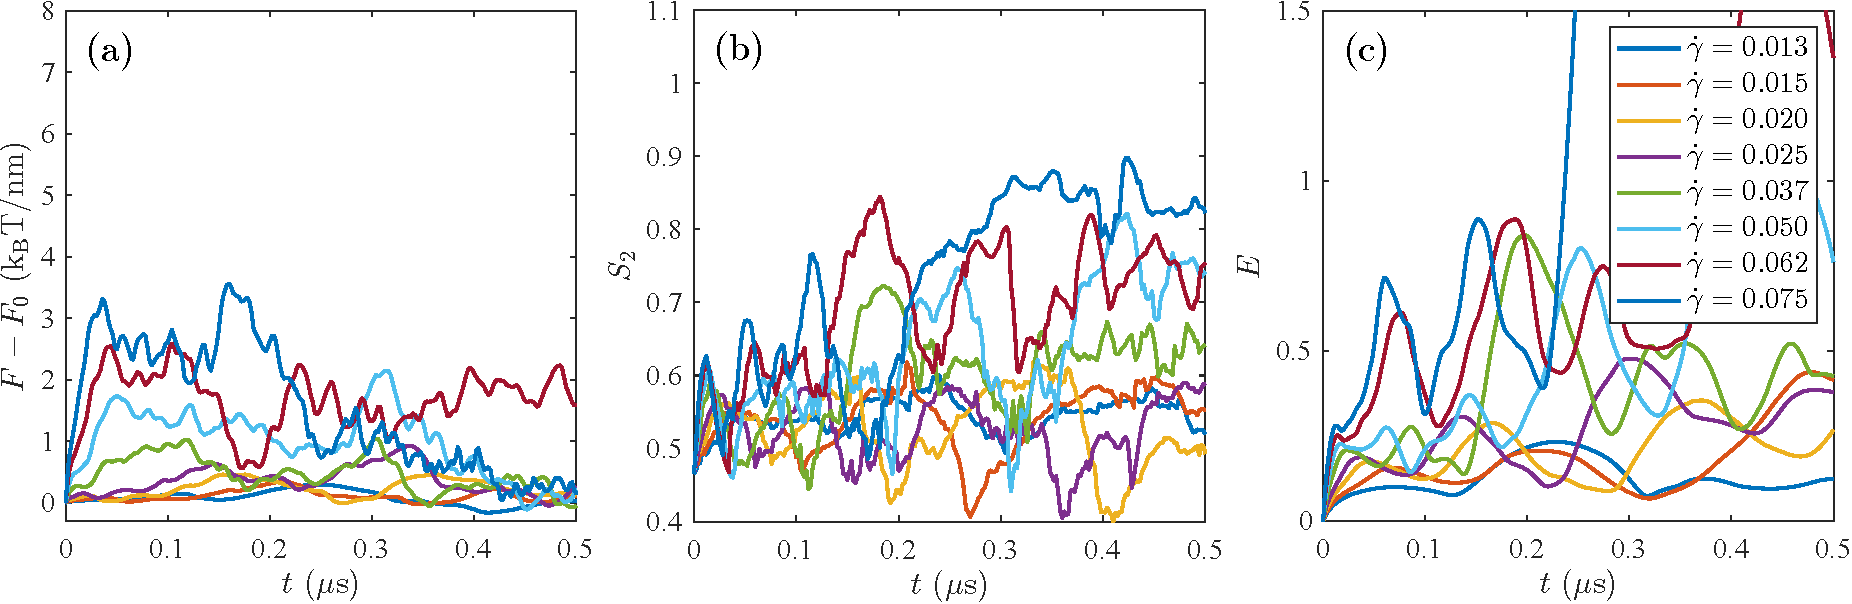
\includegraphics[width=\textwidth]{SMFigures/ULShRaw.pdf}
\end{center}
\caption{
Relative free energy $F - F_0$,
alignment $S_2$, and strain $E$ for
Type I, bilayer phase under shear flow with choices of shear rates $\dot\gamma=0.013$ -- $0.075$ ns$^{-1}$.
%The change in free energy $F$ is plotted in panel (a). Panel (b) shows the scalar order parameter $S_2$ over time $t$. Panel (c) plots the change of strain parameter $E$ in percentage over time $t$.
}
\label{fig:ulshraw}
\end{figure}


\begin{figure}[h!]
\begin{center}
\textbf{Type I, vesicle BL phase under shear flow}\par\medskip
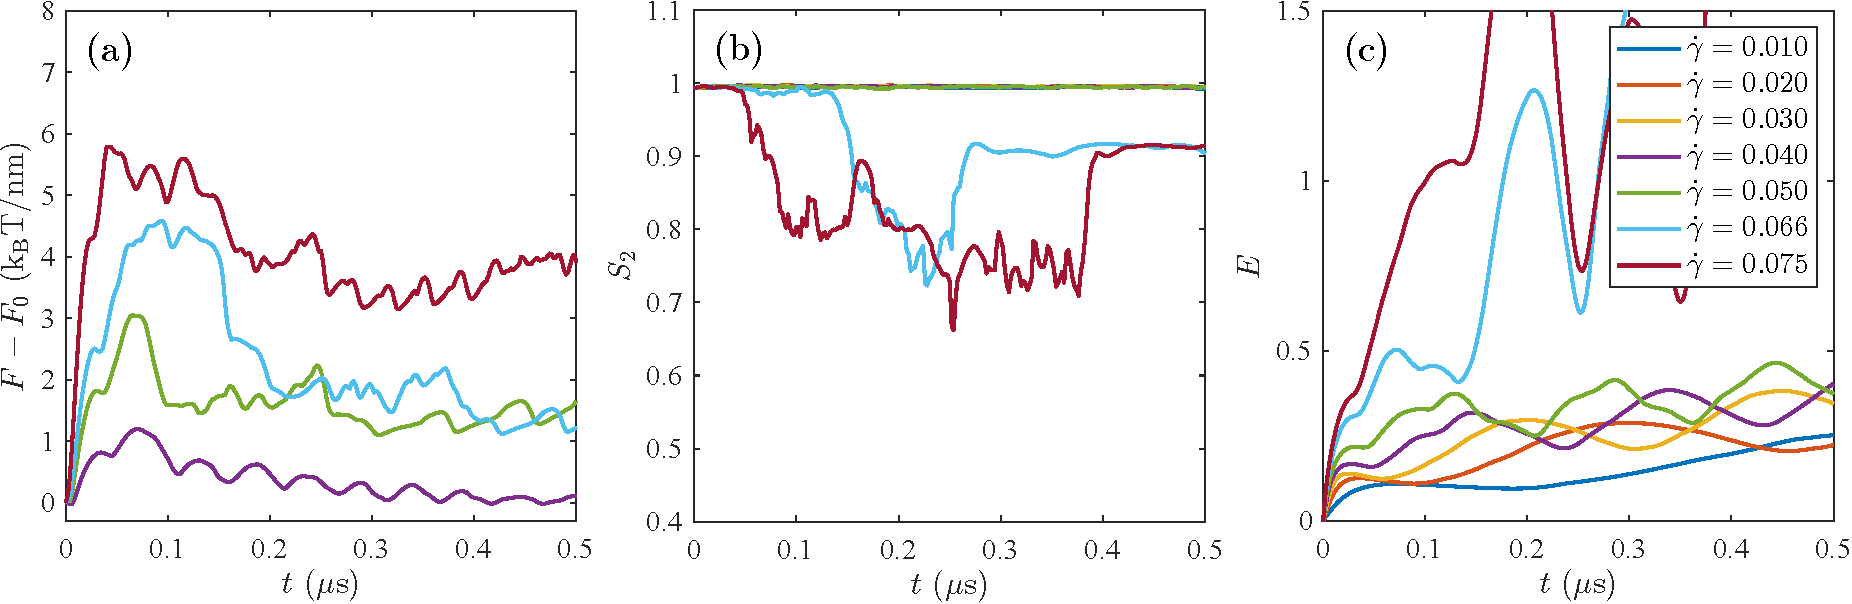
\includegraphics[width=\textwidth]{SMFigures/VeShRaw.pdf}
\end{center}
\caption{
Relative free energy $F - F_0$,
alignment $S_2$, and strain $E$ for
Type I, bilayer phase under shear flow with choices of shear rates $\dot\gamma=0.01$ -- $0.075$ ns$^{-1}$.
The JP type is the same as for Supplementary Figure \ref{fig:ulshraw} but with a
ring-shaped, rather than disordered, bilayer for initial configuration.  
%A Vesicle under a shear flow with choices of shear rates $\dot\gamma=0.01\sim0.075$. The change in free energy $F$ is plotted in panel (a). Panel (b) shows the scalar order parameter $S_2$ over time $t$. Panel (c) plots the change of strain parameter $E$ in percentage over time $t$.
}
\label{fig:veshraw}
\end{figure}


\begin{figure}[h!]
\textbf{Type II, multilamellar phase under shear flow}\par\medskip
\begin{center}
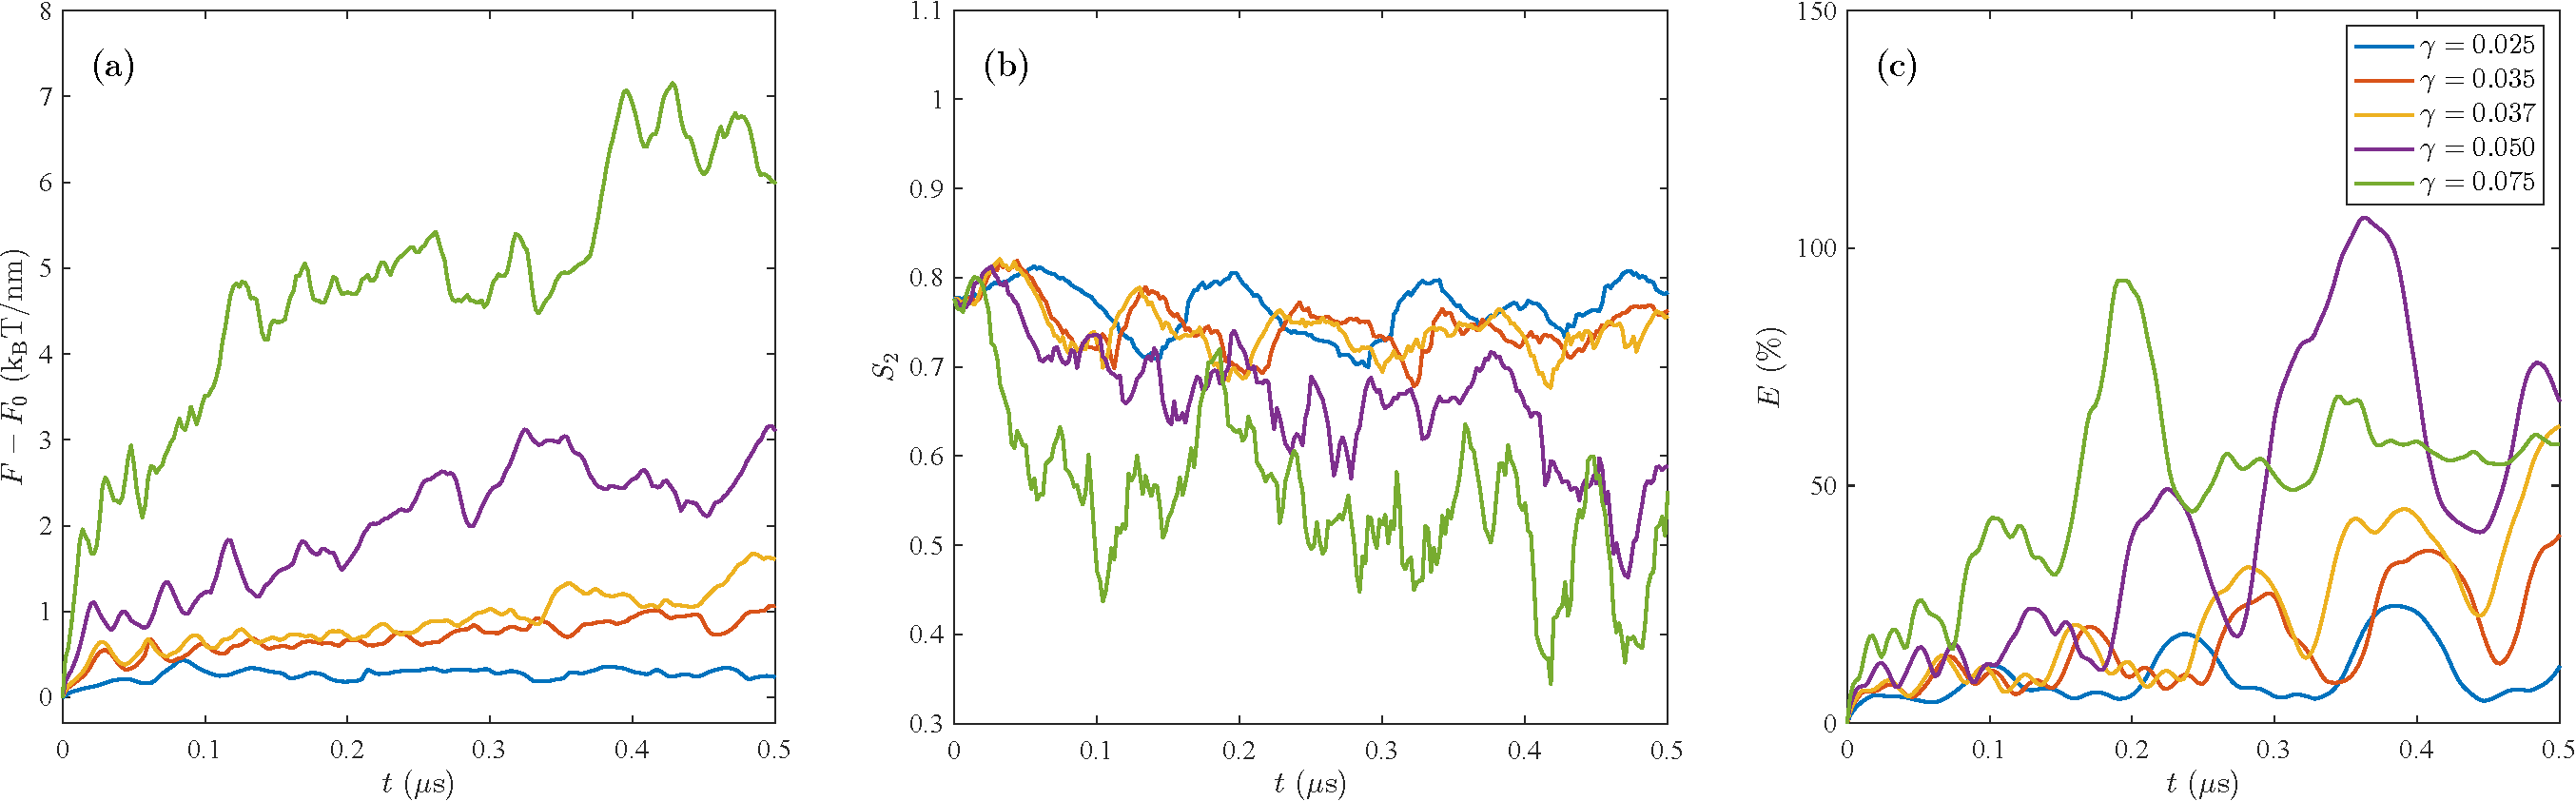
\includegraphics[width=\textwidth]{SMFigures/MLShRaw.pdf}
\end{center}
\caption{
Relative free energy $F - F_0$,
alignment $S_2$, and strain $E$ for
Type II, multilamellar phase under shear flow with choices of shear rates $\dot\gamma=0.025$ -- $0.075$ ns$^{-1}$.
%A multilamellar JP structure under a shear flow with choices of shear rates $\dot\gamma=0.025\sim0.075$. The change in free energy $F$ is plotted in panel (a). Panel (b) shows the scalar order parameter $S_2$ over time $t$. Panel (c) plots the change of strain parameter $E$ in percentage over time $t$.
}
\label{fig:mlshraw}
\end{figure}


\begin{figure}[h!]
\textbf{Type III, striated phase under shear flow}\par\medskip
\begin{center}
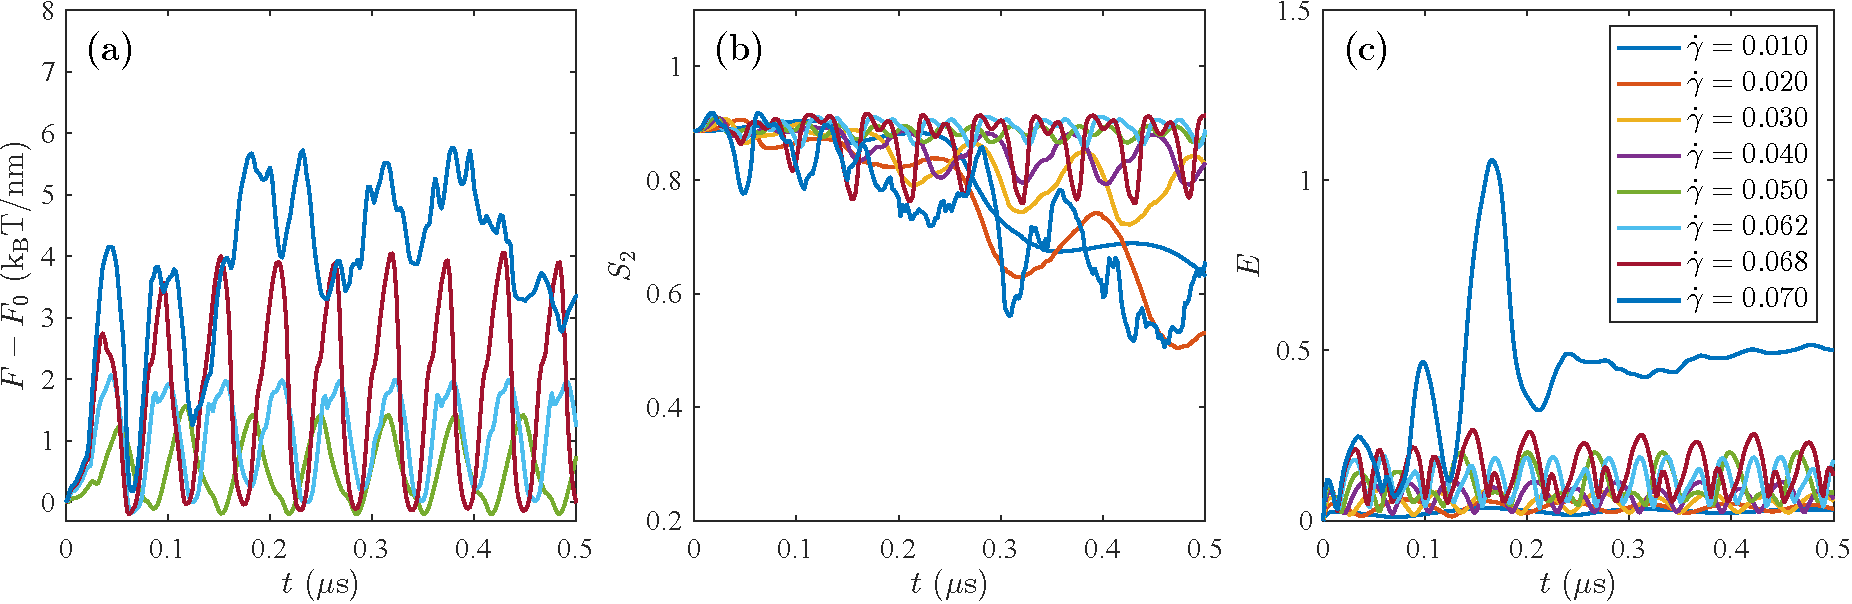
\includegraphics[width=\textwidth]{SMFigures/StShRaw.pdf}
\end{center}
\caption{
Relative free energy $F - F_0$,
alignment $S_2$, and strain $E$ for
Type III, striated phase under shear flow with choices of shear rates $\dot\gamma=0.01$ -- $0.07$ ns$^{-1}$.
%A striated JP structure under a shear flow with choices of shear rates $\dot\gamma=0.01\sim0.07$. The change in free energy $F$ is plotted in panel (a). Panel (b) shows the scalar order parameter $S_2$ over time $t$. Panel (c) plots the change of strain parameter $E$ in percentage over time $t$.
}
\label{fig:stshraw}
\end{figure}

\begin{figure}[h!]
\begin{center}
\textbf{\textsc{TG Flow Cases}}\par\medskip
\textbf{Type I, bilayer  phase under TG flow}\par\medskip
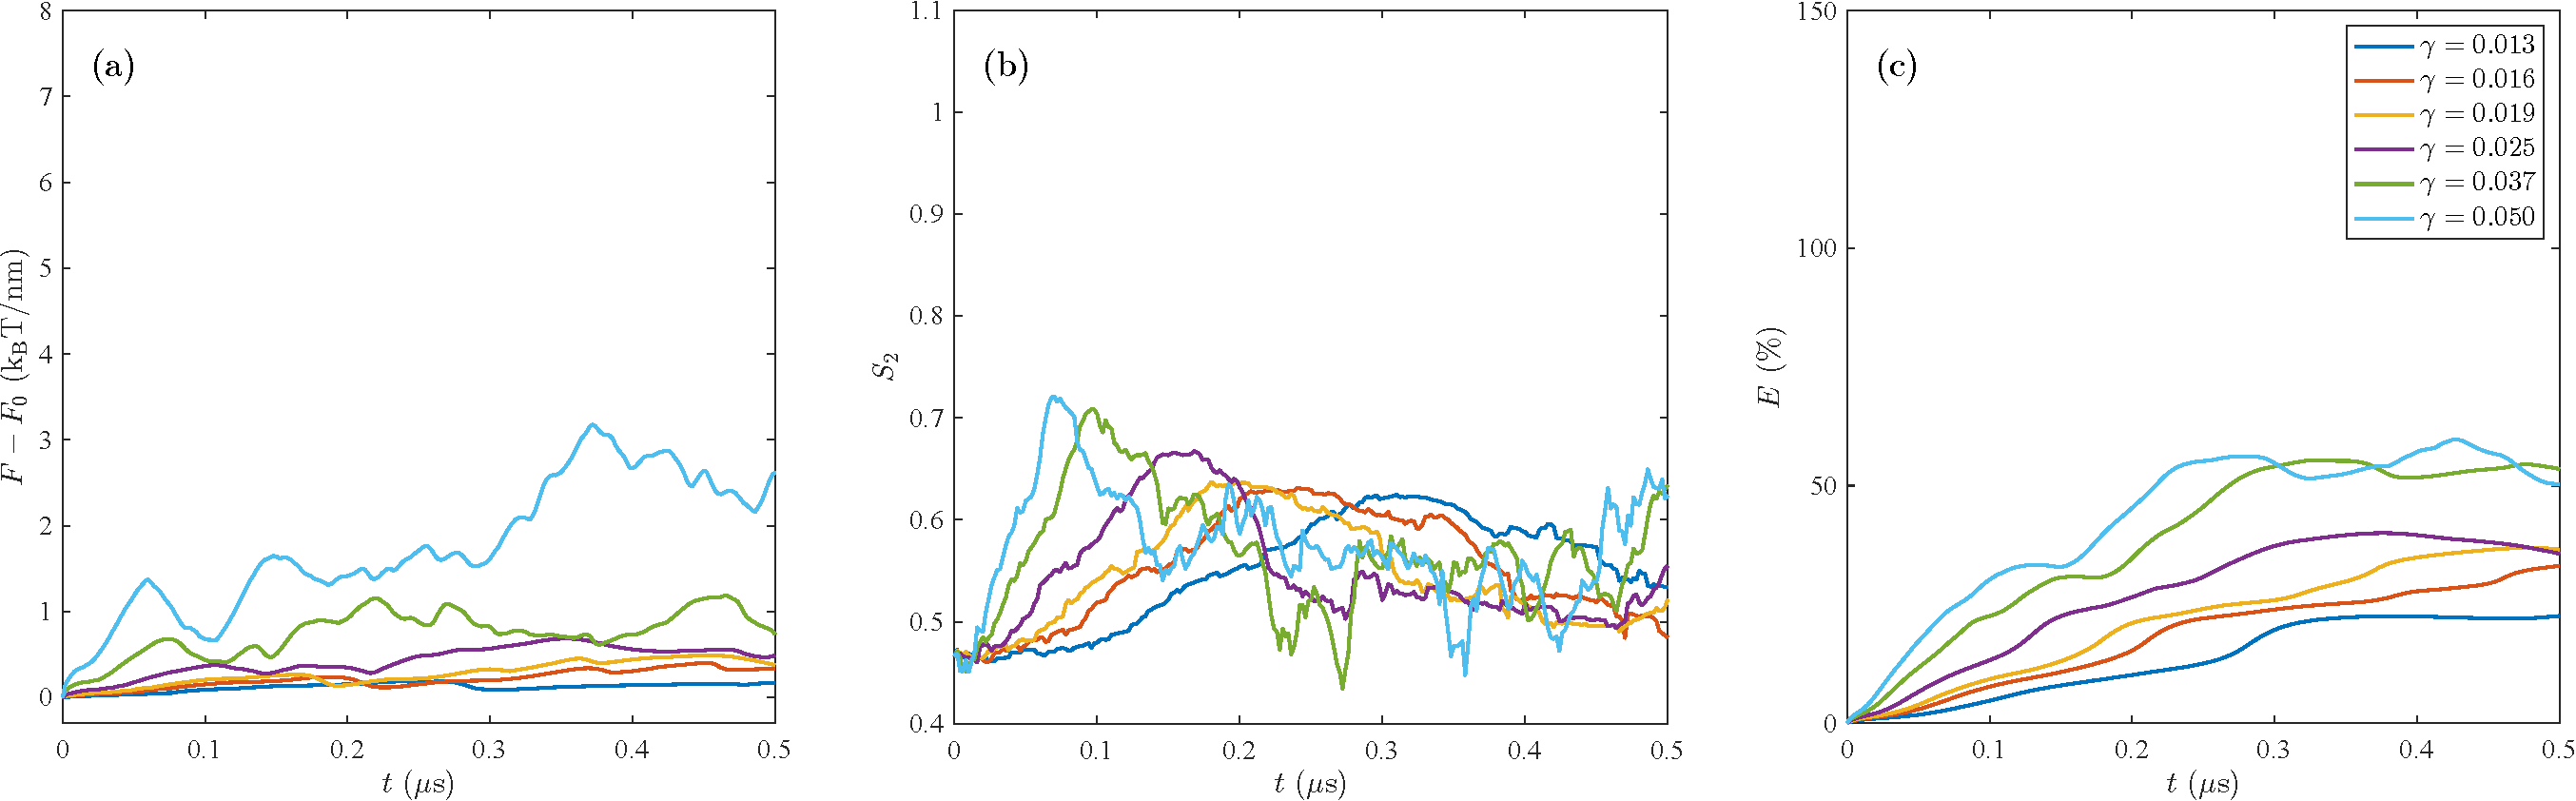
\includegraphics[width=\textwidth]{SMFigures/ULTGRaw.pdf}
\end{center}
\caption{
Relative free energy $F - F_0$,
alignment $S_2$, and strain $E$ for
Type I, bilayer phase under TG flow with choices of shear rates $\dot\gamma=0.013$ -- $0.05$ ns$^{-1}$.
%A unilamellar JP structure under a TG flow with choices of shear rates $\dot\gamma=0.013\sim0.05$. The change in free energy $F$ is plotted in panel (a). Panel (b) shows the scalar order parameter $S_2$ over time $t$. Panel (c) plots the change of strain parameter $E$ in percentage over time $t$.
}
\label{fig:ultgraw}
\end{figure}


\begin{figure}[h!]
\begin{center}
\textbf{Type I, vesicle BL phase under TG flow}\par\medskip
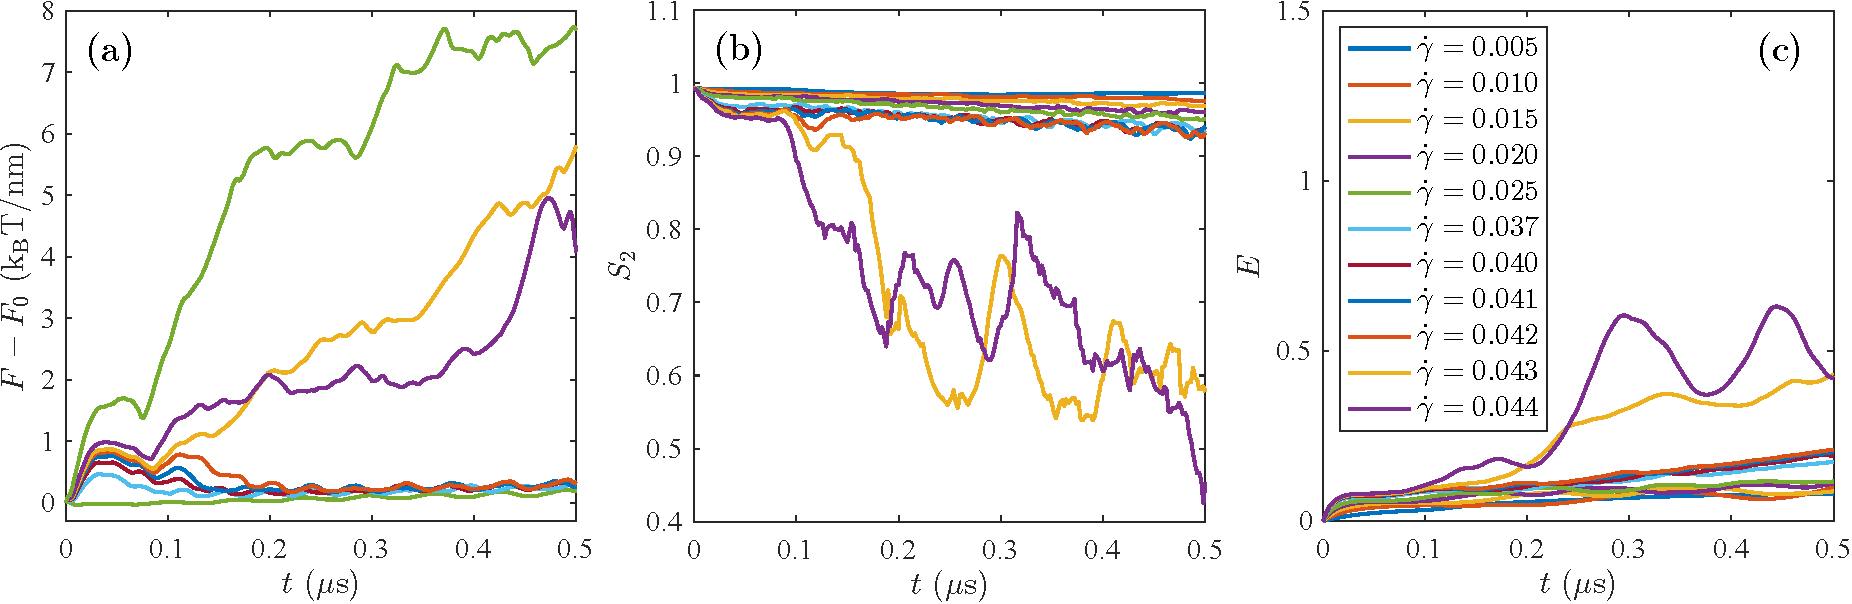
\includegraphics[width=\textwidth]{SMFigures/VeTGRaw.pdf}
\end{center}
\caption{
Relative free energy $F - F_0$,
alignment $S_2$, and strain $E$ for
Type I, vesicle bilayer phase under TG flow with choices of shear rates $\dot\gamma=0.005$ -- $0.044$ ns$^{-1}$.
The JP type is the same as for Supplementary Figure \ref{fig:ultgraw} but with a
ring-shaped, rather than disordered, bilayer for initial configuration.  
%A vesicle JP structure under a TG flow with choices of shear rates $\dot\gamma=0.005\sim0.044$. The change in free energy $F$ is plotted in panel (a). Panel (b) shows the scalar order parameter $S_2$ over time $t$. Panel (c) plots the change of strain parameter $E$ in percentage over time $t$.
}
\label{fig:vetgraw}
\end{figure}




\begin{figure}[h!]
\begin{center}
\textbf{Type II, multilamellar phase under TG flow}\par\medskip
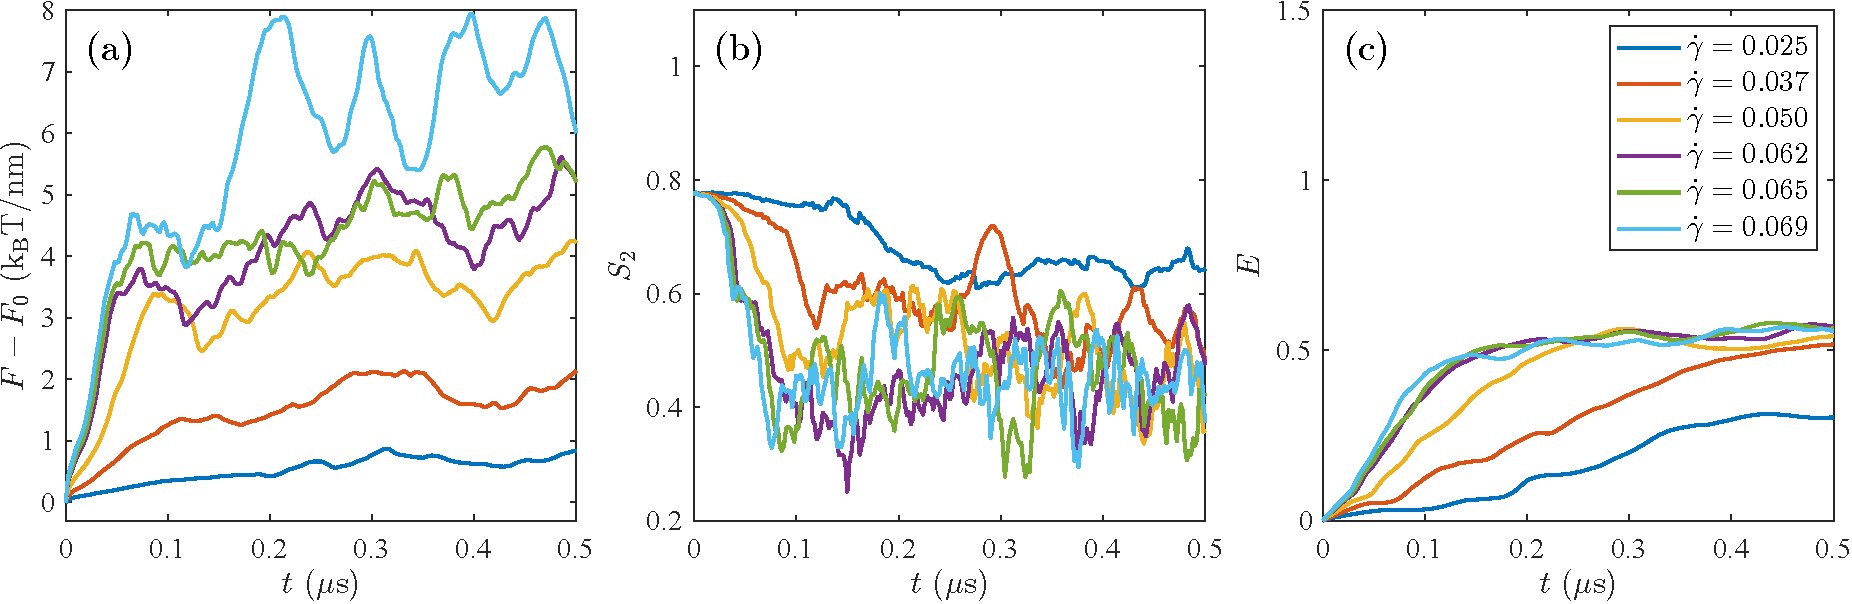
\includegraphics[width=\textwidth]{SMFigures/MLTGRaw.pdf}
\end{center}
\caption{
Relative free energy $F - F_0$,
alignment $S_2$, and strain $E$ for
Type II, multilamellar phase under TG flow with choices of shear rates $\dot\gamma=0.025$ -- $0.069$ ns$^{-1}$.
%A multilamellar JP structure under a TG flow with choices of shear rates $\dot\gamma=0.025\sim0.069$. The change in free energy $F$ is plotted in panel (a). Panel (b) shows the scalar order parameter $S_2$ over time $t$. Panel (c) plots the change of strain parameter $E$ in percentage over time $t$.
}
\label{fig:mltgraw}
\end{figure}


\begin{figure}[h!]
\begin{center}
\textbf{Type III, striated phase under TG flow}\par\medskip
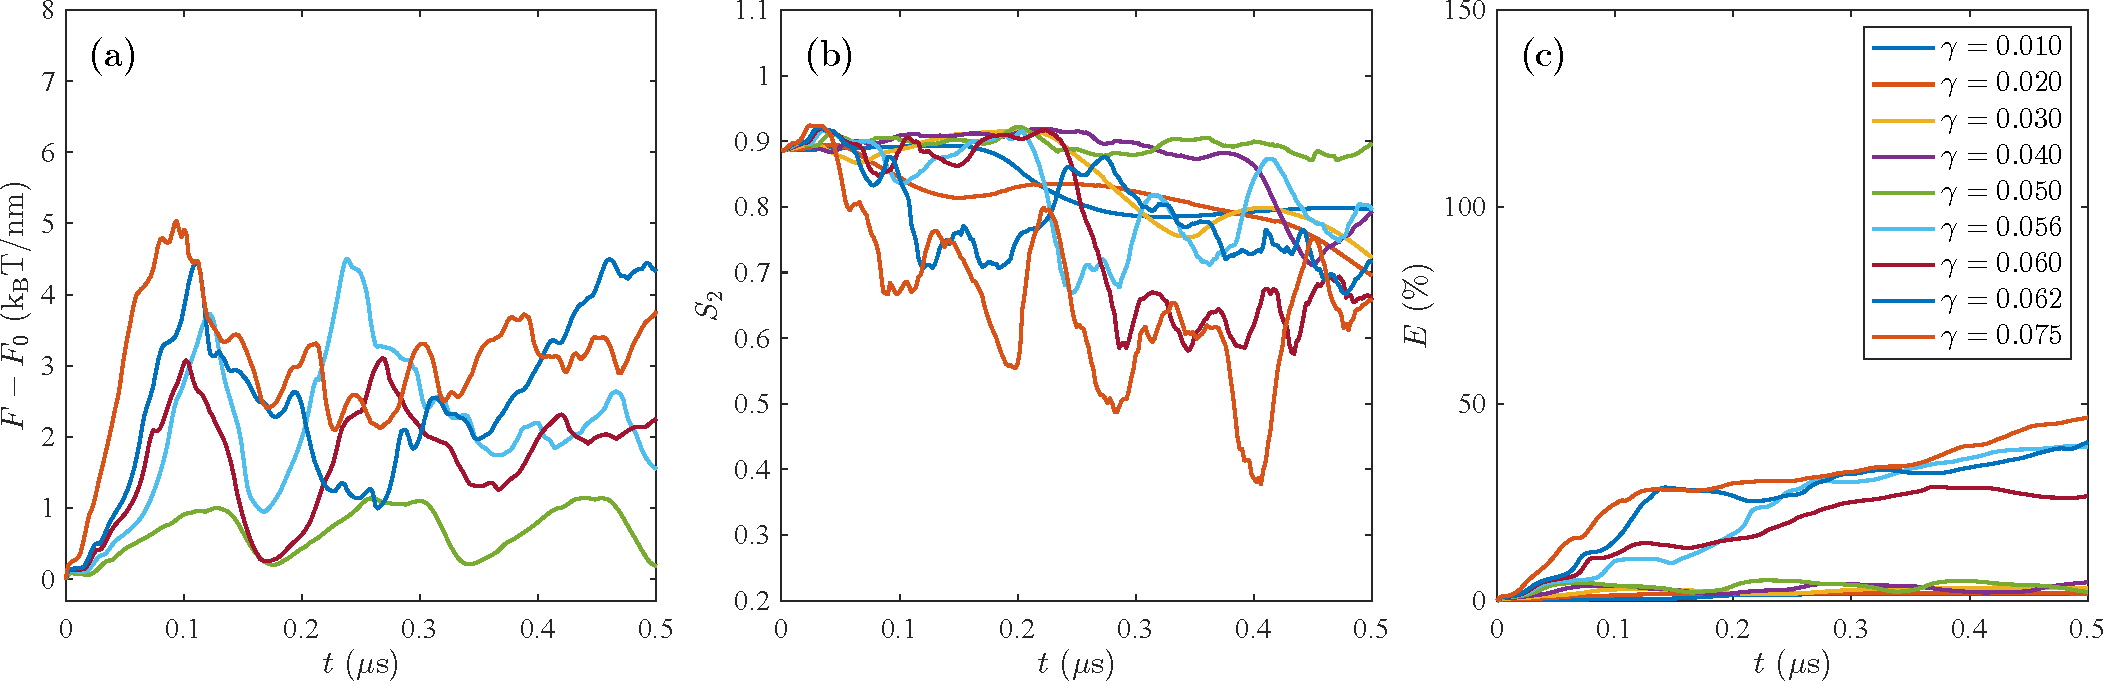
\includegraphics[width=\textwidth]{SMFigures/StTGRaw.pdf}
\end{center}
\caption{
Relative free energy $F - F_0$,
alignment $S_2$, and strain $E$ for
Type III, striated phase under TG flow with choices of shear rates $\dot\gamma=0.01$ -- $0.075$ ns$^{-1}$.
%A striated JP structure under a TG flow with choices of shear rates $\dot\gamma=0.01\sim0.069$. The change in free energy $F$ is plotted in panel (a). Panel (b) shows the scalar order parameter $S_2$ over time $t$. Panel (c) plots the change of strain parameter $E$ in percentage over time $t$.
}
\label{fig:sttgraw}
\end{figure}








\end{document}





%%%%%%%%%%%%%%%%%%%%%%%%%%%%%%%%%%%%%%%%%%%






\section{DRAFT RESULTS BELOW}
{\bf More results:}




\begin{figure}
  \begin{center}
  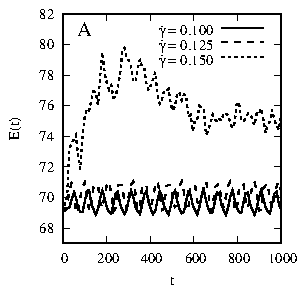
\includegraphics[width=0.3\textwidth]{CS_E.pdf}
   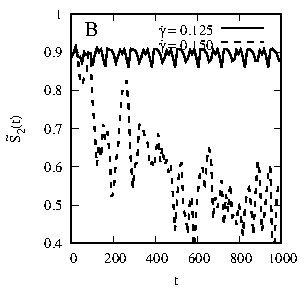
\includegraphics[width=0.3\textwidth]{CS_LOP.pdf}
    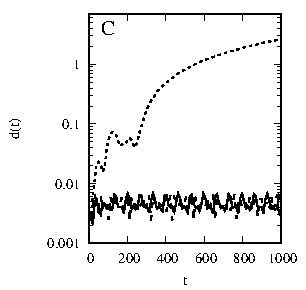
\includegraphics[width=0.3\textwidth]{CS_MSD.pdf}
  \end{center}
\caption{A checkerboard in shear flow with shear rates
  $\dot\gamma=\{0.125, 0.15\}$. We propose the order parameter defined
  by $S_{loc} = \frac12(3\cos(\theta-\bar\theta)^2-1)$}
\end{figure}


\begin{figure}
  \begin{center}
  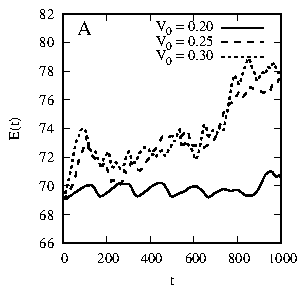
\includegraphics[width=0.3\textwidth]{CTG_E.pdf}
   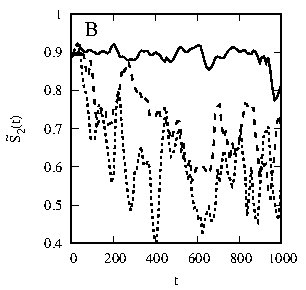
\includegraphics[width=0.3\textwidth]{CTG_LOP.pdf}
    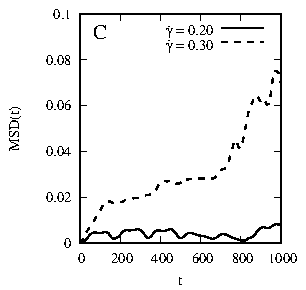
\includegraphics[width=0.3\textwidth]{CTG_MSD.pdf}
  \end{center}
\caption{A checkerboard in Taylor-Green flows when the flow strength $V_0=\{0.2,0.3\}$. }
\end{figure}






\subsubsection{}






%%%

\section{Governing Equations}
We consider a suspension of $N_b$ Janus particles in the fluid domain
$\Omega$.
The boundary of the $\Omega$ is $\bd\Omega = \Gamma_1 \cup
\cdots \cup \Gamma_{N_b}$, where $\Gamma_i$ is the boundary of Janus
particle $i$. We also consider a bounded fluid domain where $\Gamma_0$
is the fixed boundary of $\Omega$. In this case, $\bd\Omega = \Gamma_0
\cup \Gamma_1 \cup \cdots \cup \Gamma_{N_b}$.

%%%
\subsection{Hydrophobic Attraction Potential Mobility Problem} 
The mathematical formulation is a nonlinear system for the dynamics of a
collection of rigid Janus particles. For the sake of completeness, we
summarize the governing equations here, and a complete description is in
our previous work~\cite{Fu2022_JFM}. The interactions satisfy a
system of partial differential equations (PDEs) that describe the
hydrodynamic interactions and hydrophobic interactions. Assuming
inertial terms are negligible, the solvent is governed by the Stokes
equations
\begin{alignat}{3}
\label{eq:stokes}
  -\mu \Delta \uu + \nabla p &= \mathbf{0},     && \xx \in \Omega, \\
  \nabla\cdot \uu &= 0, \qquad && \xx \in \Omega, \\
  \uu - \uu_\infty &\to \mathbf{0}, && |\xx| \to \infty,
\end{alignat}
where $\uu$ is the velocity, $p$ is the pressure, $\uu_\infty$ is the
background flow, and $\mu$ is the constant viscosity. The domain $\Omega
= \Omega(t)$ is the fluid region surrounding the particles and changes
shape as the particles move. Since the particles are rigid, the solvent
velocity satisfies the no-slip rigid body motion boundary condition
\begin{align}
  \vv_i + \omega_i (\xx - \aa_i)^\perp = \uu(\xx), 
    \quad \xx \in \Gamma_i,
\end{align}
where $\vv_i$ is the translational velocity and $\omega_i$ is the
angular velocity. Once these velocities are determined, we use
second-order Adams-Bashforth to update the particle configuration. 

The translational and angular velocities guarantee that the fluid forces
balance the imposed forces. The imposed forces include the hydrophobic
interactions that arise so that particles minimize the free energy of
the structure of the surrounding water molecules. The free energy
functional is
\begin{align}
\label{eq:free_energy}
  F[u] = C \int_{\Omega} \left(\rho |\nabla u|^2 + \rho^{-1} f(u)\right)
  \,d\xx,
\end{align}
where $u$ is an order parameter for the structure of water, $\rho$ is a
decay length, $C$ is a constant, and $f(u)$ is a potential.
%$c$ is ``effective" inter-particle distance below which the steric repulsion becomes important.
Hydrogen-bond persistence times are on the order of picoseconds which is
much smaller than characteristic time for particle motion.
%\cite{MaGa13}. 
Thus we assume $u$ minimizes $F[u]$ for all times. Assuming appropriate
conditions on $f(u)$,
% (\cite{evans10}, \S 8.2),
$u$ satisfies the Euler-Lagrange equation
\begin{alignat}{3}
  \label{eq:SL}
  -\rho^2 \Delta u + \tfrac{1}{2}f'(u) &= 0, && \xx \in \Omega, \\
  u &= g, && \xx \in \bd\Omega, \\
  u &\rightarrow 0, \qquad&& |\xx| \rightarrow \infty.
\end{alignat}
Equation~\eqref{eq:SL} is solved with a boundary integral equation
method. The boundary condition $g$ is a material label that is
transported with the particle.

The particles lower the free energy $F[u]$ of the surrounding water
by moving. We calculate the rate of change of $F[u]$ using
variation of the domain. % ~\cite{Fu2018_SIAM,Bandle2015, Schiffer1954, Grinfeld2010}.
Carrying out this variation yields the stress  
\begin{align}
  \label{eq:stress}
\mathbf{T}
= C \left[ \rho^{-1} f(u) \mathbf{I}
  + \rho \left(|\nabla u|^2 \mathbf{I} - 
  2\nabla u \nabla u^T\right)\right].
\end{align}
The imposed forces and torques come from the integration of $\mathbf{T}$
along the particle boundary. These forces and torques couple the Stokes
equations \eqref{eq:stokes}, to semilinear elliptic equation
\eqref{eq:SL}. Solving for the translational and rotational velocities
gives the particle evolution.

To solve the Stokes equation with the correct boundary conditions, we
represent the velocity as the of a layer potential with Stokeslets and
rotlets
\begin{align}
  \label{eq:velocity}
  \uu(\xx) = \uu_\infty(\xx) + \DD[\eeta](\xx) + 
    \sum_{i=1}^{N_b} \left(\SS(\xx,\aa_i) \cdot \FF_i + 
    \RR(\xx,\aa_i) T_i\right), \quad \xx \in \Omega.
\end{align}
%
Then, the density function $\eeta$, translation velocity $\vv_i$ and
angular velocity $\omega_i$ satisfy
\begin{alignat}{3}
  \nonumber
  \vv_i + \omega_i (\xx - \aa_i)^\perp &= \uu_\infty(\xx)
    -\frac{1}{2} \eeta(\xx) + \DD[\eeta](\xx) \\
  \label{eq:SKIE}
    + \sum_{j=1}^{N_b} &
    \left(\SS(\xx,\aa_j) \cdot \FF_j + \RR(\xx,\aa_j) T_j\right),
    \quad &&\xx \in \Gamma_i,\: i=1,\ldots,N_b, \\
  \label{eq:mobility1}
  \int_{\Gamma_i} \eeta \, \dif s &= \mathbf{F}_i, 
  &&i = 1,\ldots,N_b, \\
  \label{eq:mobility2}
  \int_{\Gamma_i} \eeta \cdot (\xx-\aa_i)^\perp \, \dif s &= T_i,
  &&i = 1,\ldots,N_b.
\end{alignat}

\subsection{Normal Derivative of Double Layer Potential and HAP Energy}

We adopt the double layer potential to express the solution of \eqref{eq:SL} where the condition is $f(u)=u^2$. Then it is given by 
\begin{align}
\label{eq:energy_BIE}
u({\bf x}) = \DD[\sigma](\xx) = \int_\Gamma \frac{\partial G(\xx-\yy)}{\partial \nnu_\yy}\sigma(\yy)\, \dif s_\yy,
\end{align}
%
where $G(\xx)$ is the fundamental solution to the screened Laplace
equation \eqref{eq:SL} and $\nnu_\yy$ is the outward normal.
Since the free energy functional can be written as 
\begin{align}
\label{eq:free_energy2}
  E[u(\xx)] &= C\rho \int_\Gamma u \frac{\partial u}{\partial \nnu}  \,\dif s, \quad \xx\in\Gamma_i,
\end{align}
%
we can then refer to the identity (\cite{Hsiao2008}, \S 1.2) to calculate this boundary integral equation without evaluating the normal derivative of the double layer potential directly.

Consider
\begin{align}
\nnu_\xx \cdot \nabla_\zz u(\zz) &=\nnu_\xx \cdot \nabla_\zz \int_\Gamma \frac{\partial G(\zz-\yy)}{\partial \nnu_\yy}\sigma(\yy) \,\dif s_\yy\\
&=\int_\Gamma \nnu_\xx\cdot \left(\nabla_\zz\nabla_\yy^\top  G(\zz-\yy)\right)\cdot \nnu_\yy\sigma(\yy)  \,\dif s_\yy\\
&=-\int_\Gamma \nnu_\xx\cdot \left(\nabla_\yy\nabla_\yy^\top G(\zz-\yy)\right)\cdot\nnu_\yy\sigma(\yy)\ \dif s_\yy\\
&=-\int_\Gamma {\bf t}_\xx\cdot\Delta_\yy G(\zz-\yy) {\bf t}_\yy \sigma(\yy)\ \dif s_\yy+\int_\Gamma({\bf t}_\xx\cdot\nabla_\yy)({\bf t}_\yy\cdot\nabla_\yy G(\zz-\yy))\sigma(\yy)\ \dif s_\yy\\
&= -\int_\Gamma {\bf t}_\xx\cdot\frac1\rho^2 G(\zz-\yy) {\bf t}_\yy \sigma(\yy)\ \dif s_\yy - 
({\bf t}_\xx\cdot\nabla_\zz)\int_\Gamma \frac{\partial G(\zz-\yy)}{\partial s_\yy}\sigma(\yy)\ \dif s_\yy\\
&= -\frac1\rho^2 {\bf t}_\xx\cdot \int_\Gamma G(\zz-\yy){\bf t}_\yy \sigma(\yy)\ \dif s_\yy + 
({\bf t}_\xx \cdot \nabla_\zz)\int_\Gamma G(\zz-\yy)\frac{\partial \sigma(\yy)}{\partial s}\ \dif s_\yy.
\end{align}
%
Here ${\bf t}_\xx$ is the tangent vector at the point $\xx$ and $d/ds$ is the arclength derivative.
Letting $\zz\to\xx\in\Gamma$, we obtain
%
\begin{equation}
\label{eq:normal_deriv}
\frac{\partial}{\partial \nnu_\xx} \DD[\sigma](\xx) = -\frac1\rho^2 {\bf t}_\xx\cdot \SSS[\sigma{\bf t}](\xx) + \frac{\partial}{\partial s}\SSS\left[\frac{\partial \sigma}{\partial s}\right](\xx).
\end{equation}
%

Substituting \eqref{eq:normal_deriv} to \eqref{eq:free_energy2} provides the total energy calculation
throughout this paper and this expression takes the advantage of not calculating the quadruple layer potential which has well-known obstacle in numerical implementation.

%Suppose we split the solution to the screened Laplace boundary value problem~\eqref{eq:SL}
%into smooth portion $w_i$ and singular portion $u_i$. That is, 
%\begin{equation}
%w_i({\bf x}) = u({\bf x}) - u_i = u({\bf x}) - \int_{\Gamma_i }\left(\pderiv{}{\nnu_\yy}
%    K_0 \left(\frac{|\xx - \yy|}{\rho}\right)\right) \sigma_i(\yy) \,
%    \dif s_\yy, \quad \xx \in \Gamma_i.
%\end{equation}
%Consider the case when $f(u)=u^2$ in~\eqref{eq:free_energy}, we can rewrite the free energy functional as 
%
%\begin{align}
%\label{eq:free_energy2}
%  E[u(\xx)] &= C\rho \sum_{i=1}^{N_b}\int_{\Gamma_i} u \frac{\partial u}{\partial \nnu}  \,\dif s
%= C\rho\sum_{i=1}^{N_b}\int_{\Gamma_i} u \left(\frac{\partial w_i}{\partial \nnu}+\frac{\partial u_i}{\partial \nnu} \right) \, \dif s, \quad \xx\in\Gamma_i.
%\end{align}
%%%%
%Follow the divergence theorem on the last term in the equation above and denote $g_i(x)$ as the boundary data on $\Gamma_i$, we obtain
%\begin{align}
%\label{eq:free_energy3}
%  E[u(\xx)] &= C\rho\sum_{i=1}^{N_b}\left(\int_{\Gamma_i} u \frac{\partial w_i}{\partial \nnu} \,\dif s  + \int_{\mathbb{R}^n\setminus \overline{U}_i} \left( \nabla u \cdot\nabla u_i + u\Delta u_i\right) \,\dif \xx\right)\\
%%
%&= C\rho\sum_{i=1}^{N_b}\left(\int_{\Gamma_i} u \frac{\partial w_i}{\partial \nnu} \,\dif s  + \int_{\mathbb{R}^n\setminus \overline{U}_i} u\Delta u_i\,\dif \xx
%+\int_{\Gamma_i}\left(u+\frac12\sigma\right)\frac{\partial u_i}{\partial \nnu} \,\dif s     
%- \int_{\mathbb{R}^n\setminus \overline{U}_i} u\Delta u_i\,\dif \xx \right)\\
%&= C\rho\sum_{i=1}^{N_b}\left(\int_{\Gamma_i} u \frac{\partial w_i}{\partial \nnu} + 
%\left(g_i+\frac12\sigma_i\right)\frac{\partial u_i}{\partial \nnu}   \,\dif s \right), \quad \xx \in \Gamma_i.
%\end{align}
%
%
%

%  &= C\rho\sum_{i=1}^{N_b}\left(\int_{\Gamma_i} g_i \frac{\partial w_i}{\partial \nnu} 
% +  \left(u_i+\frac12\sigma\right)  \frac{\partial g_i}{\partial \nnu} \,\dif s - \int_{\mathbb{R}^n\setminus \overline{U}_i}\Delta g_i  \left(u_i+\frac12\sigma\right)  - g_i \left(u_i+\frac12\sigma\right) \,\dif \xx\right) \\
% &= C\rho\sum_{i=1}^{N_b}\int_{\Gamma_i} g_i \frac{\partial w_i}{\partial \nnu}+ \left(u_i+\frac12\sigma\right)  \frac{\partial g_i}{\partial \nnu}\,\dif s, \quad \xx\in\Gamma_i.



%%
%$\sigma$ satisfies the second-kind integral equation
%\begin{equation}
%\label{eq:screenedSKIE}
%  g(\xx) = \frac{1}{2}\sigma(\xx) + 
%    \frac{1}{2\pi}\int_{\bd\Omega} \left(\pderiv{}{\nnu_\yy}
%    K_0 \left(\frac{|\xx - \yy|}{\rho}\right)\right) \sigma(\yy) \, 
%    \dif s_\yy, \quad \xx \in \bd\Omega,
%\end{equation}

\section{Numerical Results}

\subsection{Self-Assembled Janus Particle with Specific Boundary Conditions}

Distinct morphologies can be obtained from 
the HAP model by shifting the boundary condition $g(\xx)$.
Consider the linear case where $f(u) = u^2$.
This choice makes \eqref{eq:SL} a boundary value
problem for the screened-Laplace equation
and the solutions have a boundary layer structure that decays to $0$ in the
bulk with the decay length $\rho$.
We consider three kinds of boundary conditions
on particle $\Gamma_i$:
\begin{equation}
  \label{eq:bcs}
  \begin{tabular}{c|c|c}
     \text{(i)} & \text{(ii)} & \text{(iii)} \\
    \hline
    \rule{0pt}{4ex} 
      $g(\mathbf{x}) = \displaystyle \frac{1+\cos (\theta_i(\xx))}{\sqrt{3\pi r}}$
    & $g(\mathbf{x}) = \displaystyle \frac{2+\cos (\theta_i(\xx))}{\sqrt{9\pi r}}$
    & $g(\mathbf{x}) = \displaystyle \frac{\cos (\theta_i(\xx))}{\sqrt{\pi r}}$
\end{tabular}
\end{equation}
The number $\theta_i(\xx)$ is the angle formed by the position $\xx$,
the particle center $\aa_i$, and the particle director $\dd_i$.
(Figure~\ref{fig:flow_map}). The normalizations e.g., $(\pi r)^{-1/2}$,
provide a uniform surface energy $\int_{\Gamma_i} g^2 \,ds = 1$ for
circular particles of radius $r$. The cases (ii) and (iii) are obtained
by applying a vertical shift and scaling to case (i). Using this setup,
we simulate the dynamics of 60 particles with one set of random initial
positions and orientations as shown in Figure~\ref{fig:relax}(a)

\begin{figure}
  \begin{center}
  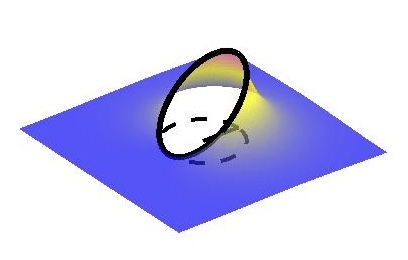
\includegraphics[width=0.2\textwidth]{LPA.jpg}
  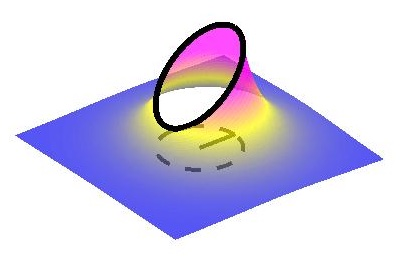
\includegraphics[width=0.2\textwidth]{LPB.jpg}
  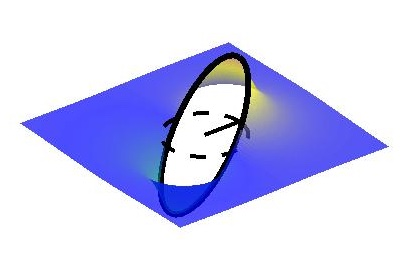
\includegraphics[width=0.2\textwidth]{LPC.jpg}
  \end{center}
  \vspace{-20pt}  
  \caption{\label{fig:bcs} Boundary conditions characterize the water
  structure at the particle interface: an amphiphilic particle (left), a
  hydrophobic particle with anisotropic intensity (middle), a water
  structure with positive/negative charge (right). The dashed curve is
  the boundary of the disk and the arrow is its director for each
  particle.}
\end{figure}


\begin{figure}
  \begin{center}
  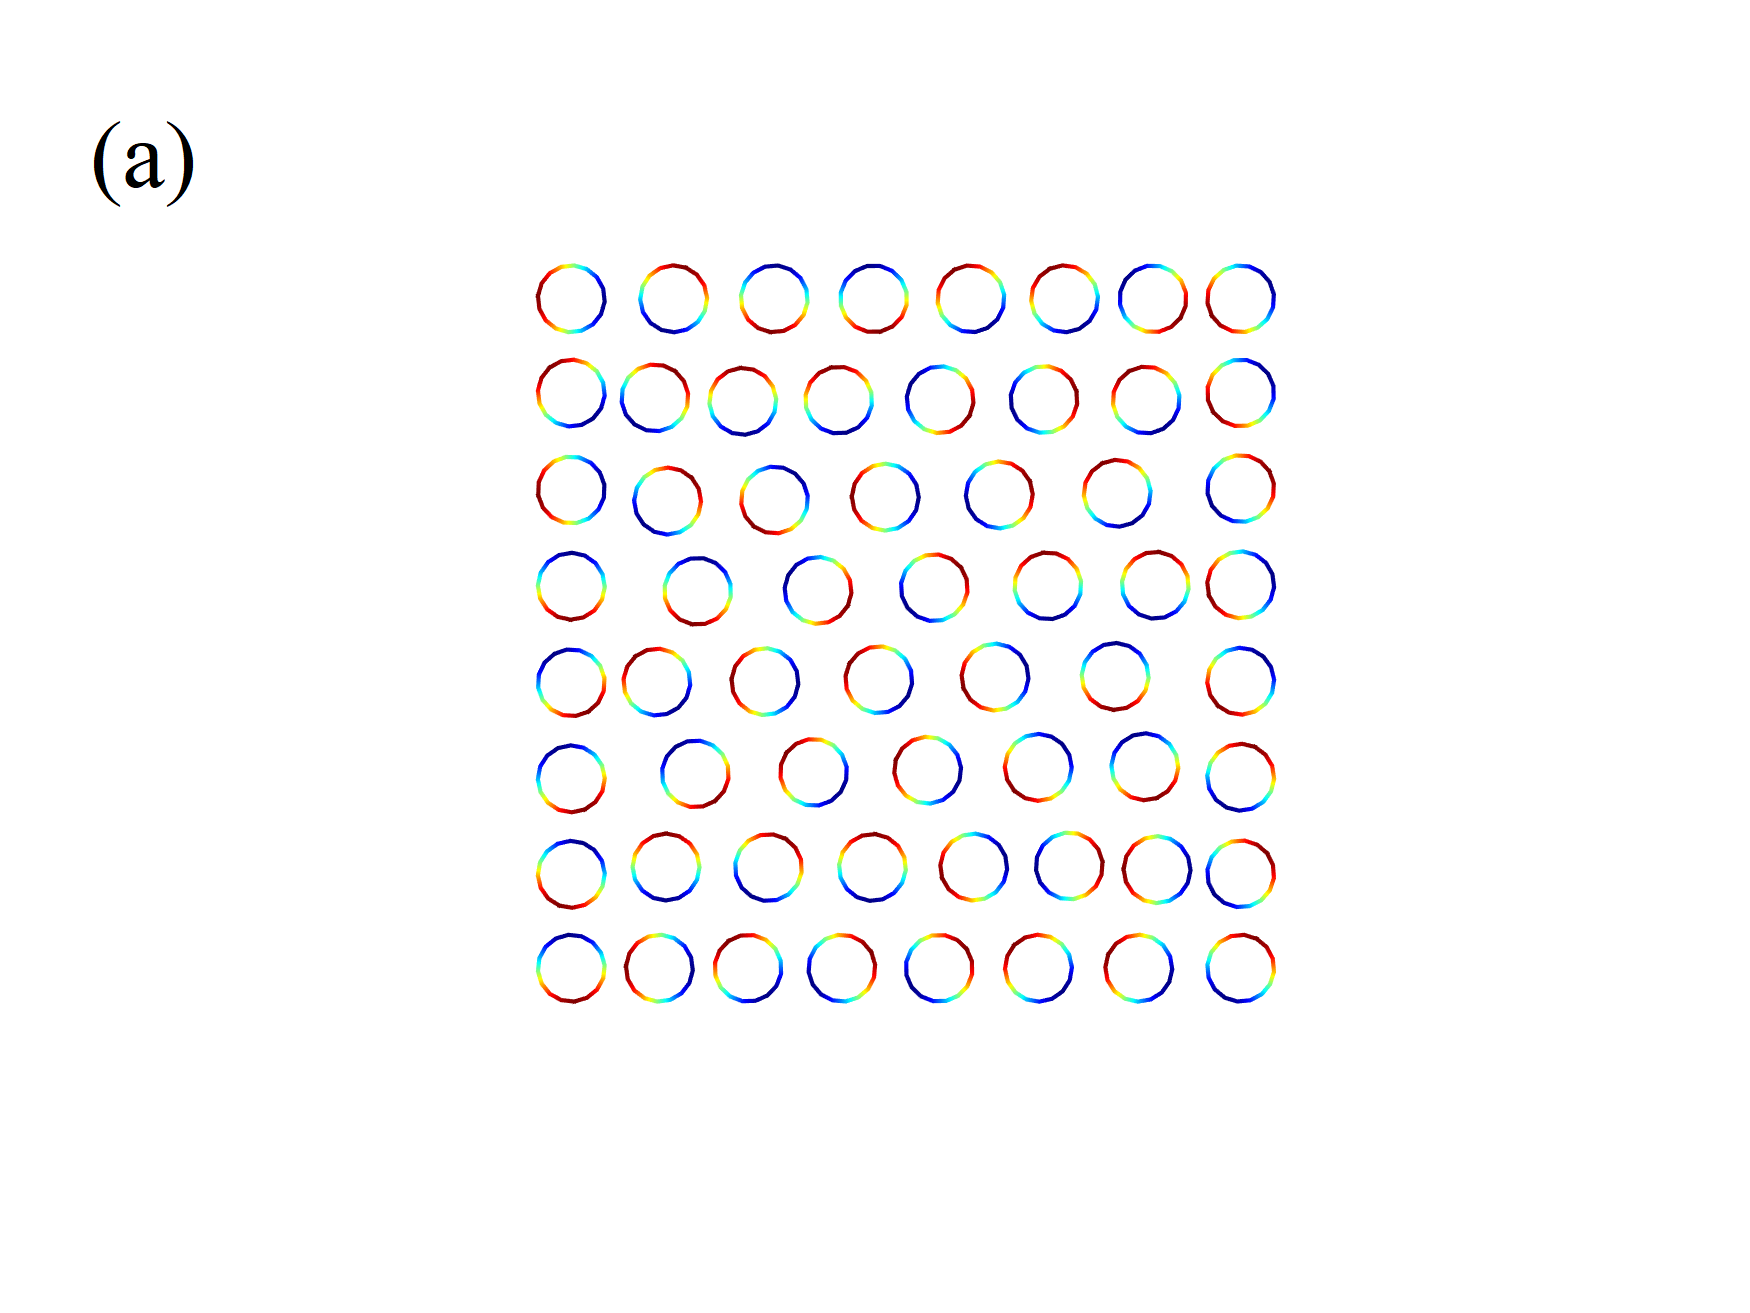
\includegraphics[width=0.4\textwidth]{Fig2a.png}
  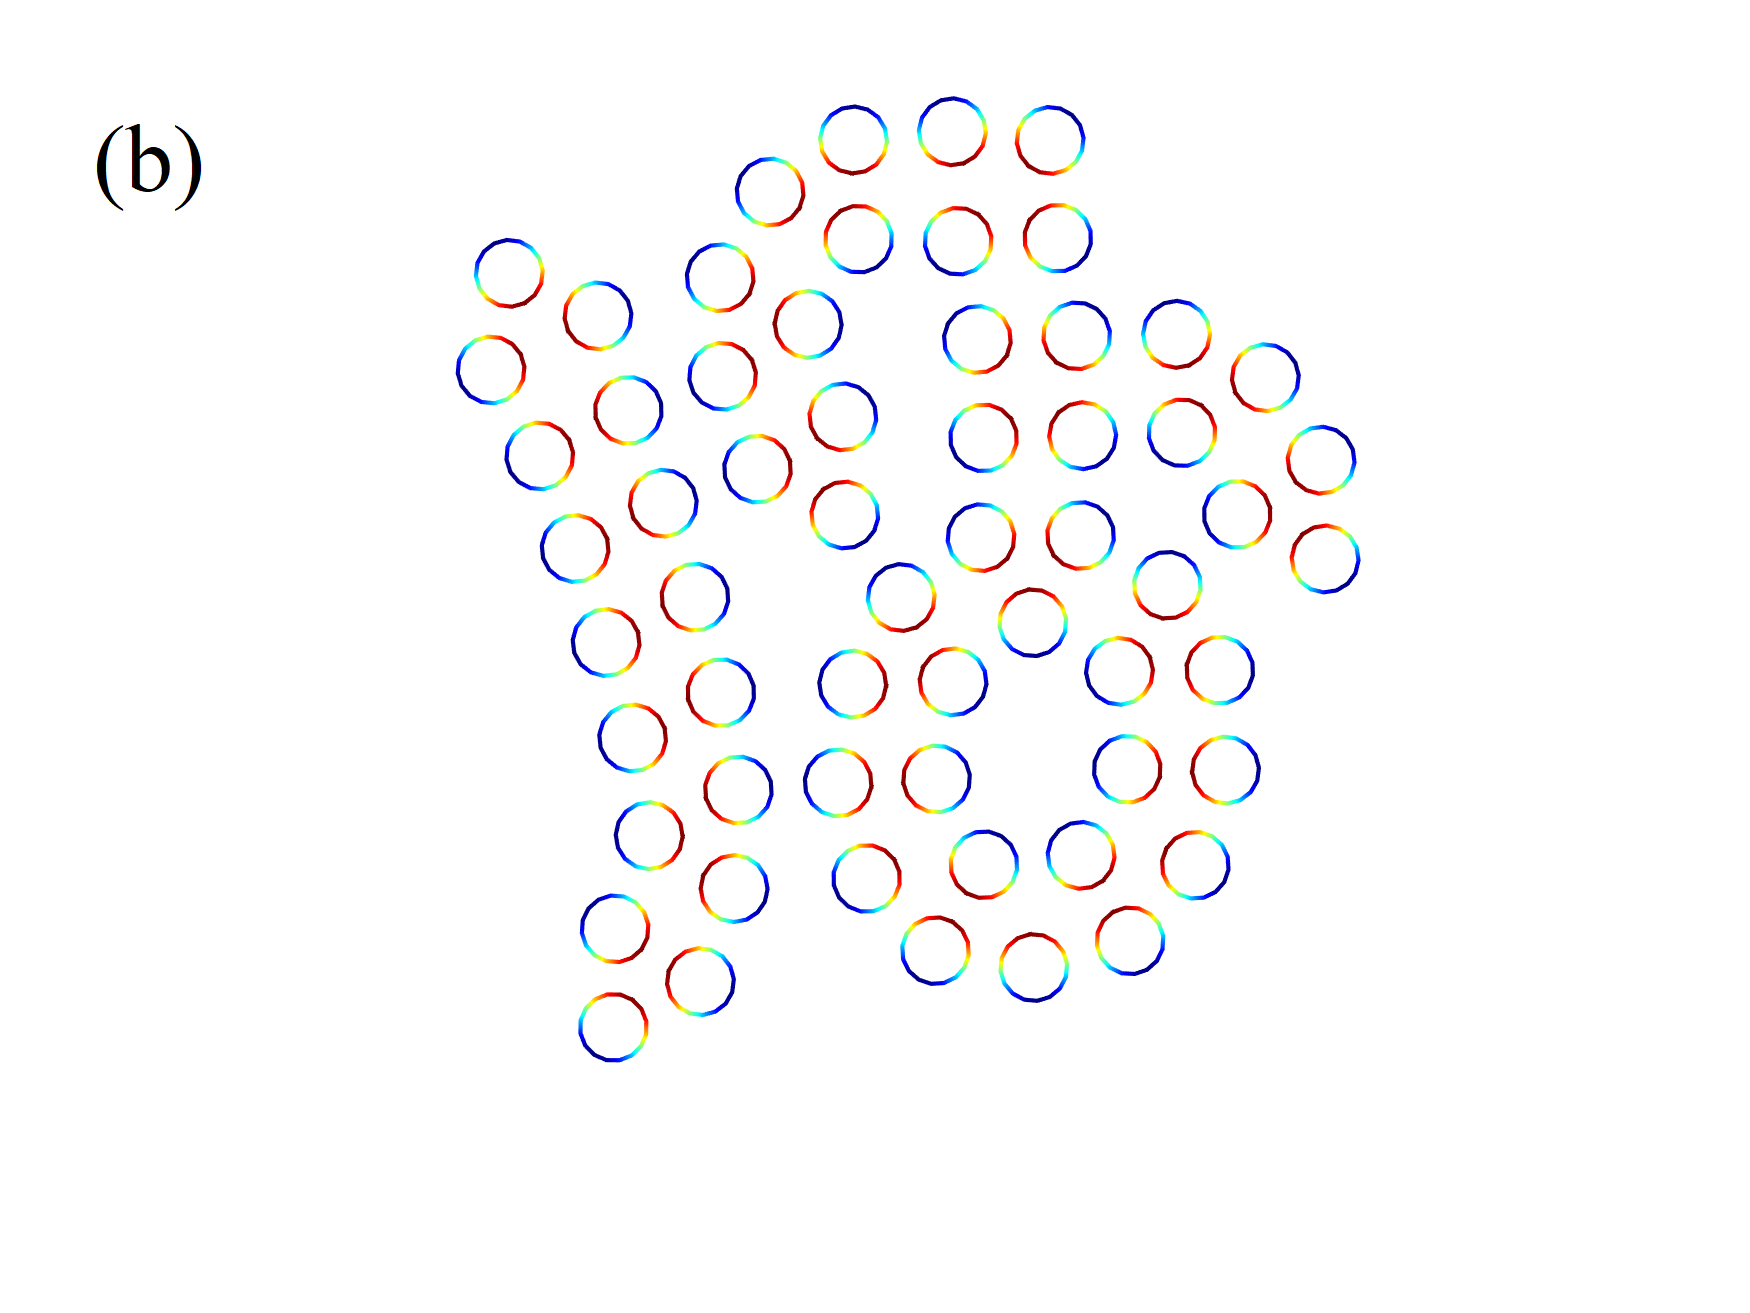
\includegraphics[width=0.4\textwidth]{Fig2b.png}\\
  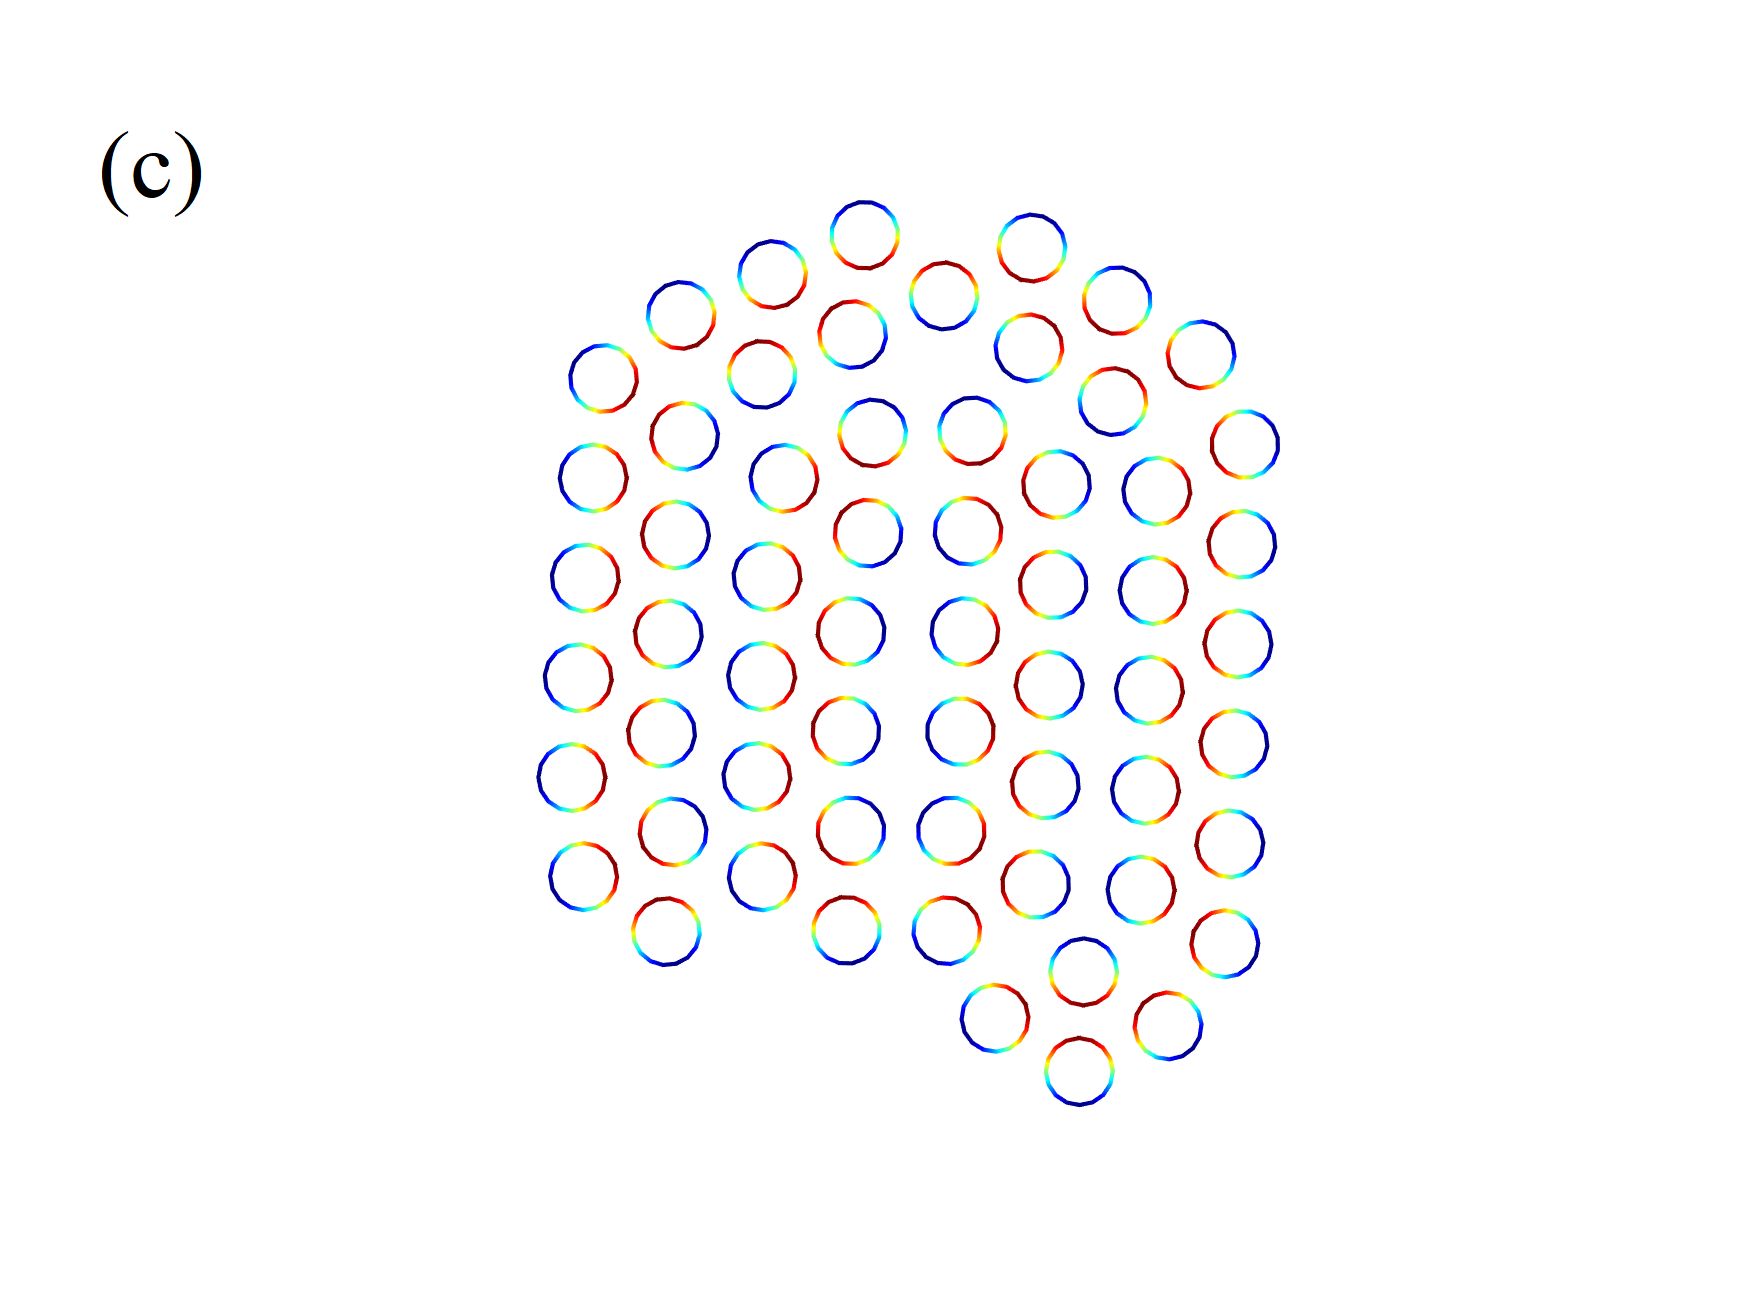
\includegraphics[width=0.4\textwidth]{Fig2c.png}
  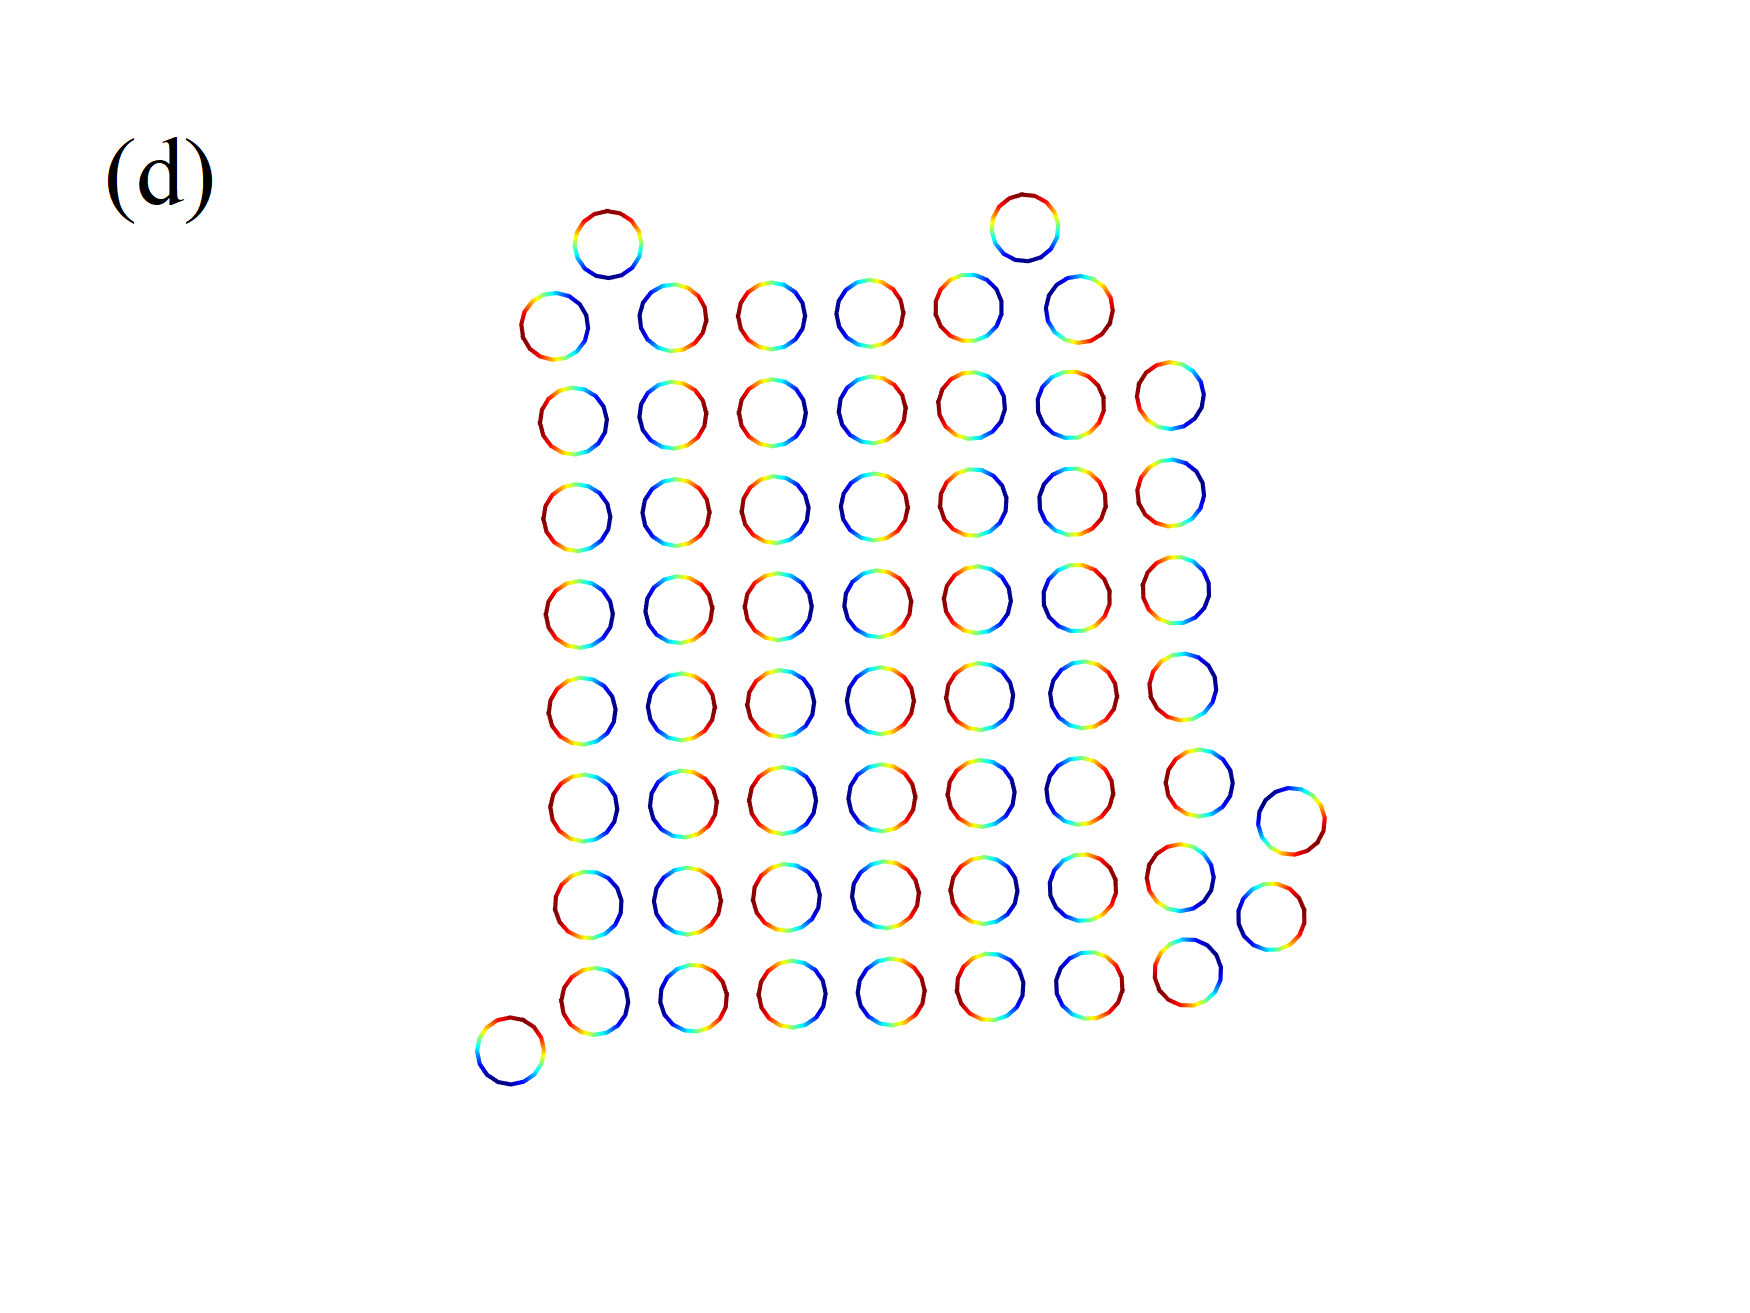
\includegraphics[width=0.4\textwidth]{Fig2d.png}
  \end{center}
  \vspace{-20pt}  
  \caption{\label{fig:relax} (a) Initial configuration for $N_b=60$
  structures. In order to expedite the self-assembly procedure, all
  particles are placed in a $8\times8$ box initially. (b)--(d)
  Equilibrium states for all boundary conditions~\eqref{eq:bcs}(i)--(iii), respectively. Colors represent the boundary values that increases from minimum (blue) to maximum (red).  Panel (b) reaches the equilibrium at $t=1200$; Panel (c) reaches the steady-state at $t=600$; Panel (d) reaches the final state at $t=180$.}
\end{figure}



\begin{figure}
  \begin{center}
  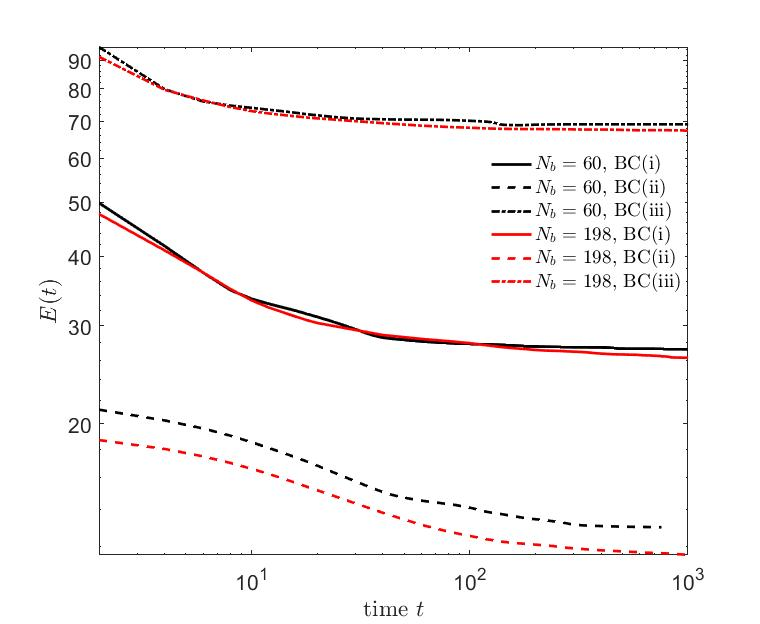
\includegraphics[width=0.5\textwidth]{Relax_Energy.jpg}
  \end{center}
  \vspace{-20pt}  
  \caption{\label{fig:relax_energy} Energy profile for all three boundary conditions.}
\end{figure}

Case (i) models amphiphilic particles.
Amphiphilic particles have a hydrophobic tail and a hydrophilic head
and these are accounted for as follows.
The hydrophilic side takes the value $u =0$.
This mimics the apolar head of a lipid, for example, which does
not alter the structure of adjacent waters. The hydrophobic side
represents hydrocarbons and takes the value 
$u > 0$. The interaction between particles is attractive,
and particles will collectively orient their tails toward
one another. Fig~\ref{fig:relax}(b) demonstrates multiple bilayer structures such as pancake and vesicle shapes.


Multilamelar bilayers arise when both sides of the particle 
are hydrophobic. 
The boundary condition \eqref{eq:bcs}(ii) 
gives a particle with a hydrophobic intensity that is greater
on the $\theta_i = 0$ side than on the $\theta_i = \pi$ side.
The initial self-assembly is similar to that in case (i).
The difference arises in the long-time dynamics where the bilayers
no longer remain well-separated. 
Rather, the bilayers form layers 
as a consequence of the interfacial tension of exposed particle
heads.%~\cite{Huetal19, deMeetal21}. 
Fig~\ref{fig:relax}(c) shows the multilamellar structure with 8 layers when $N_b=60$. 
The number of folds depends on several factors, for instances, number of
particles and initial configurations.


Finally, boundary condition \eqref{eq:bcs}(iii) models 
a particle whose head surface repels the tail surface as proposed in
\cite{MaRa76, Ma77}.
The particles initially form chains with their directors perpendicular to the
length of the chain. The equilibrium structure
resembles a checkerboard pattern
where each particle coordinates
its head with the head of three other particles and its tail with the
tail of three other particles. % Fig~\ref{fig:self-assembly}(c).
Fig~\ref{fig:relax}(d) gives an example that this boundary condition results a checker board/stripes equilibrium state.


Fig~\ref{fig:relax_energy} shows the energy profile of boundary conditions (i)--(iii) using 
\eqref{eq:free_energy2} with \eqref{eq:normal_deriv} for normal derivative expression. As expected, for all simulation runs, the total energy of the systems decreases and reaches equilibrium states.



\subsection{Collective Janus Particles Suspended in a Shear Flow}
%%%


Consider placing the equilibrium state of boundary condition \eqref{eq:bcs} (ii) for 60 particles in a shear flow,
\begin{equation}
\uu_\infty(\xx) = \dot\gamma ({\bf e}_y\cdot\xx){\bf e}_x,
\end{equation}
%
where $\dot\gamma$ is the shear rate. Fig~\ref{fig:shear_1} (a)--(c) show the snapshots of simulation results when $\dot\gamma=0.05$.
We measure the ratio of major and minor axes $\lambda$ by adopting an ellipse fitting using the singular value decomposition and track this aspect ratio for this multi-lamellar structure when the flow is on. 
The result is shown in panel (d) and we observe that the multi-lamellar structure will be slightly stretched and the aspect ratio $\lambda=3.5$ increases over time.
%
Notice that for this simulation, the center of mass position of the
initial configuration is not at the origin and it is slightly to the
right of the origin. We also track the aspect ratio $\lambda$ for the
case that the center of mass position is shifted to the origin. Panel
(d) also shows that the dynamics of two sets of simulations are
invariant of center of mass position in a shear flow.

%
\begin{figure}
  \begin{center}
  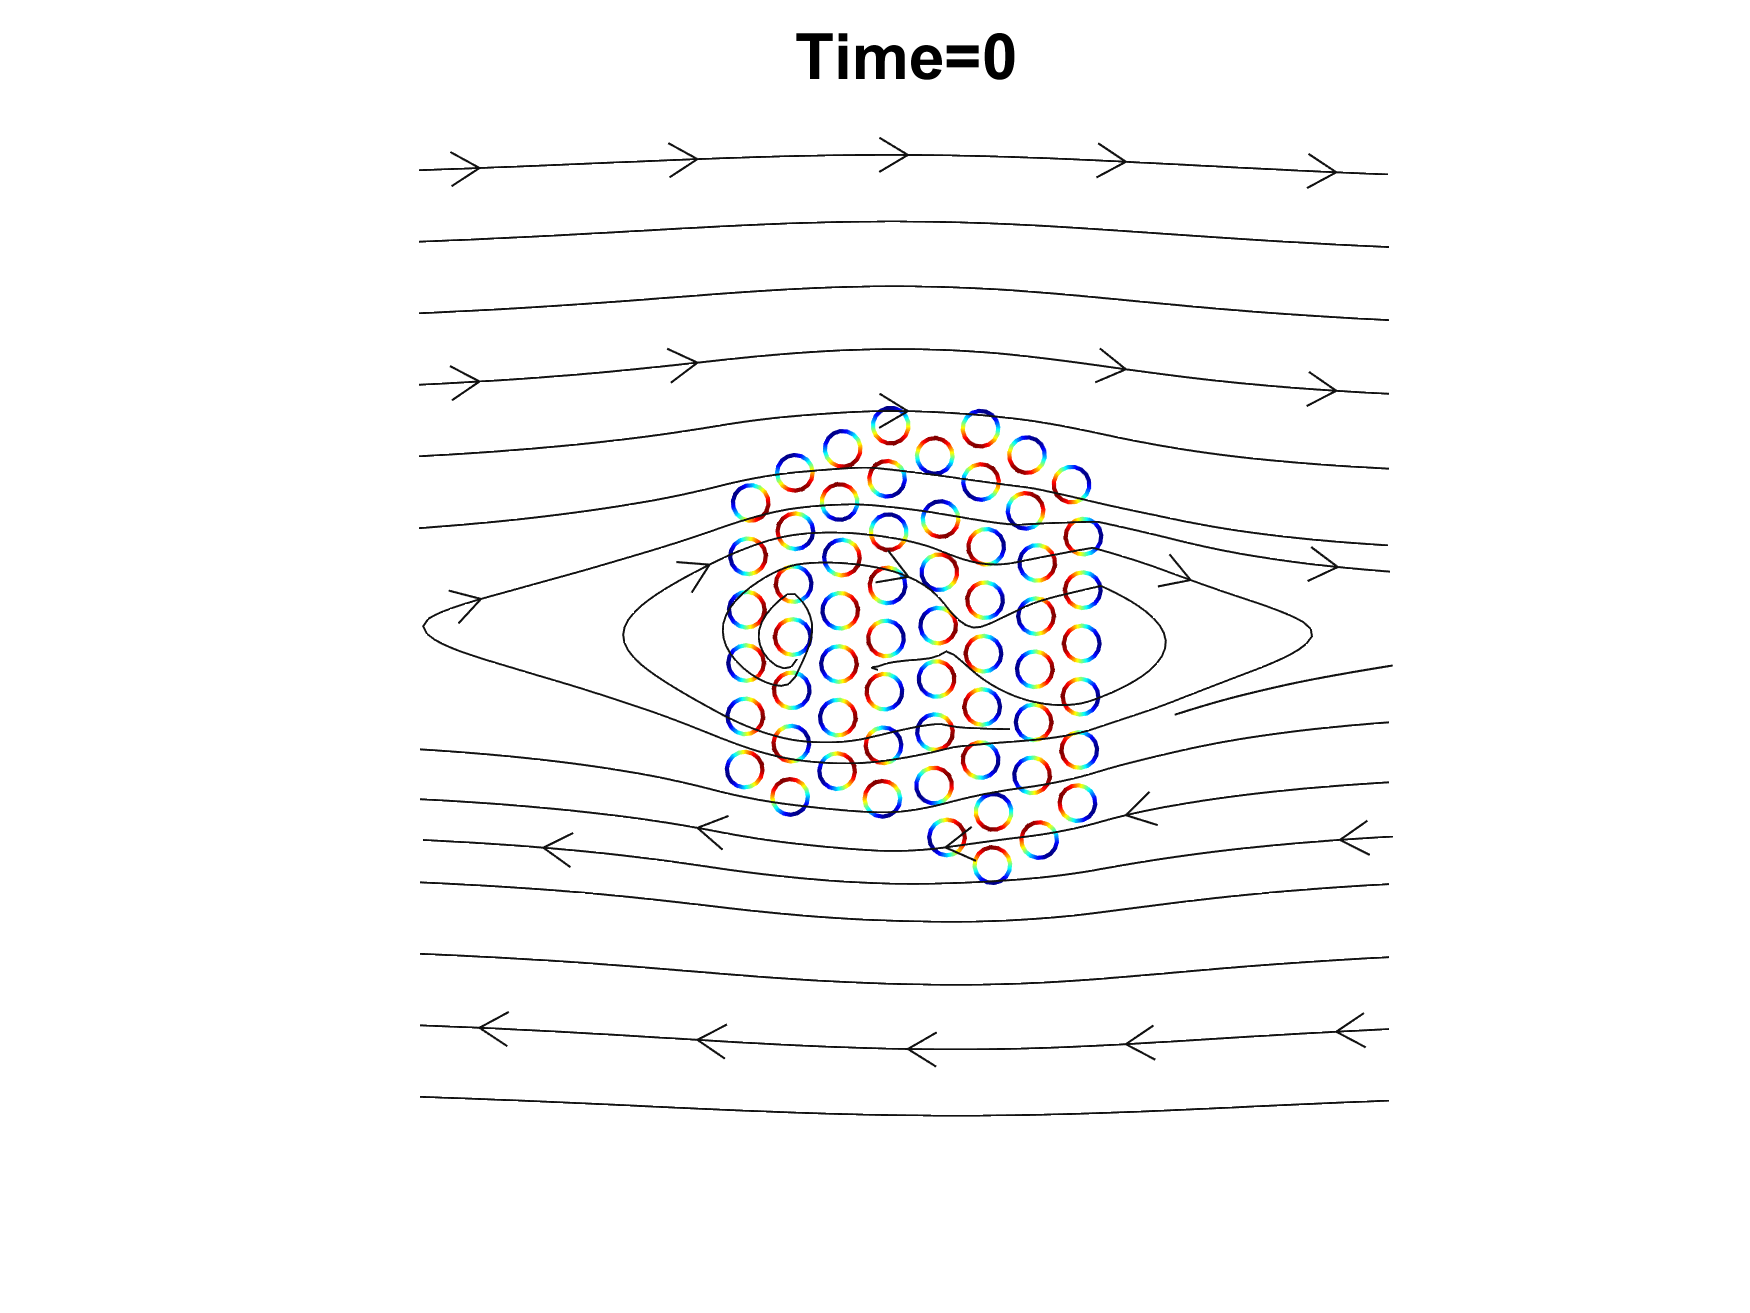
\includegraphics[width=0.21\textwidth]{shear_0.png}
  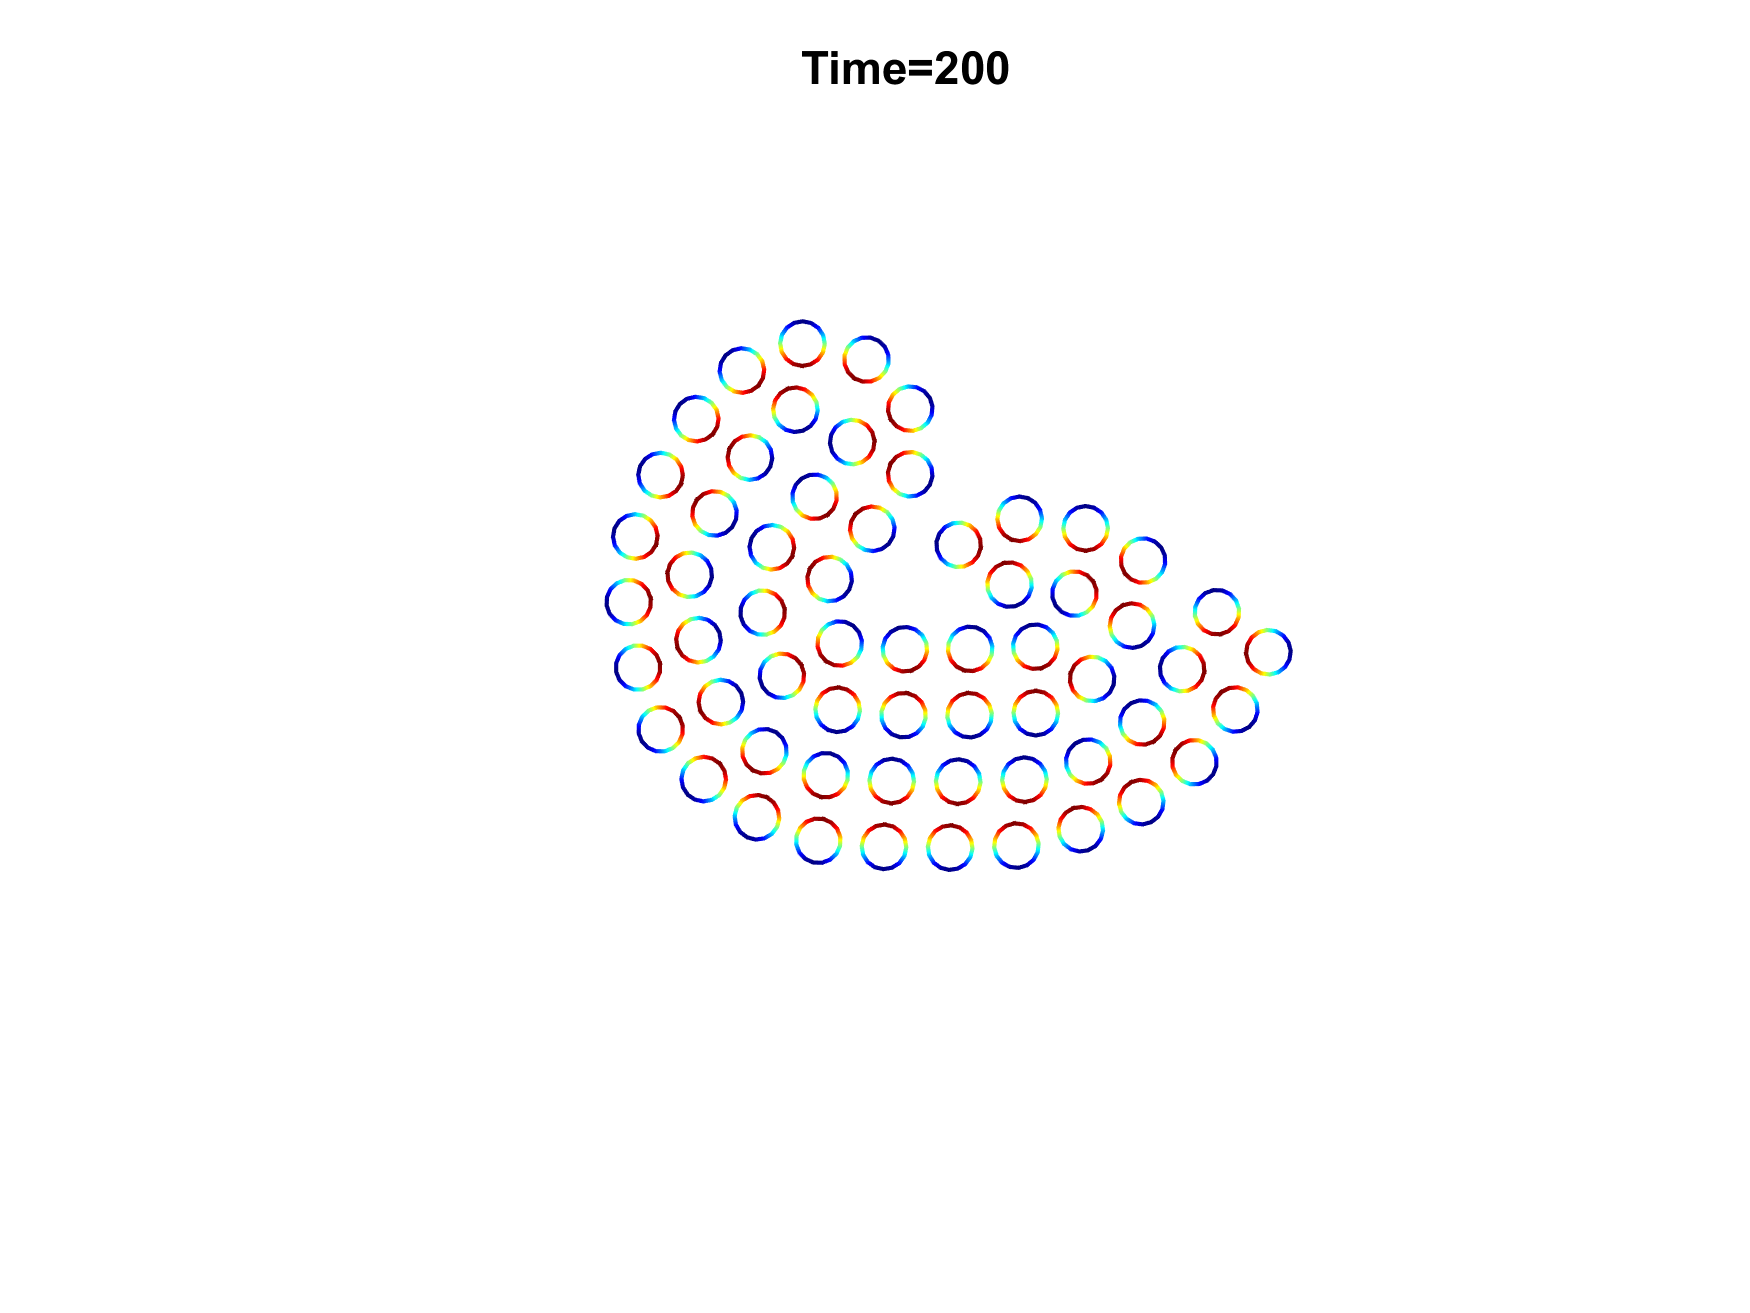
\includegraphics[width=0.21\textwidth]{shear_1000.png}
  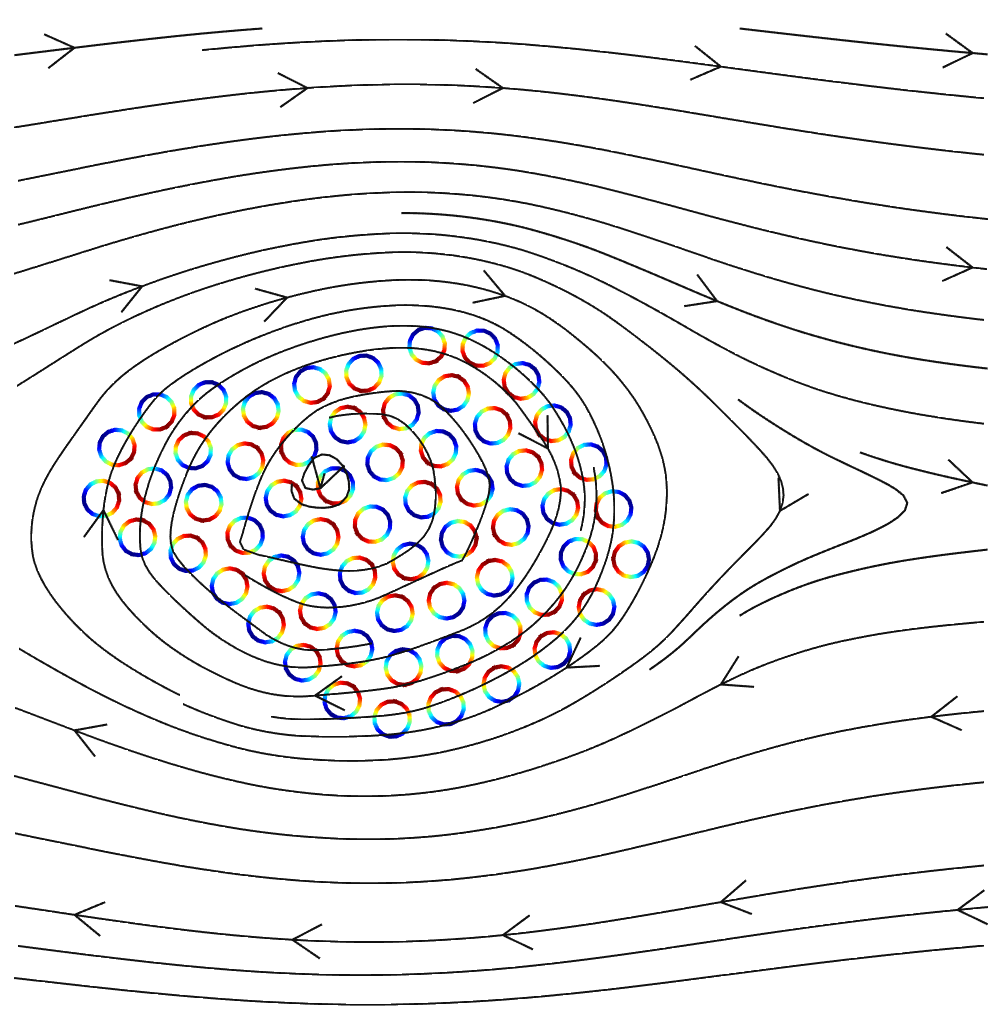
\includegraphics[width=0.21\textwidth]{shear_2000.png} 
  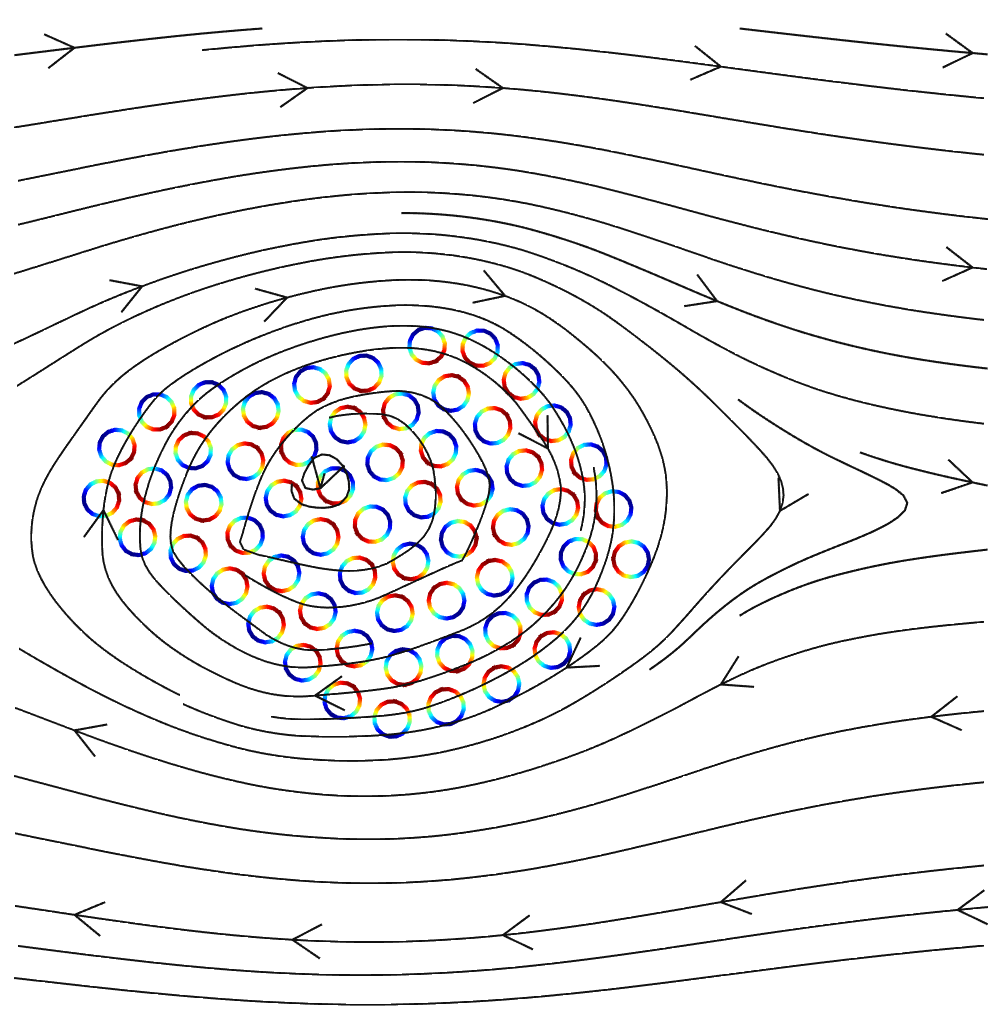
\includegraphics[width=0.21\textwidth]{shear_2000.png} \\
  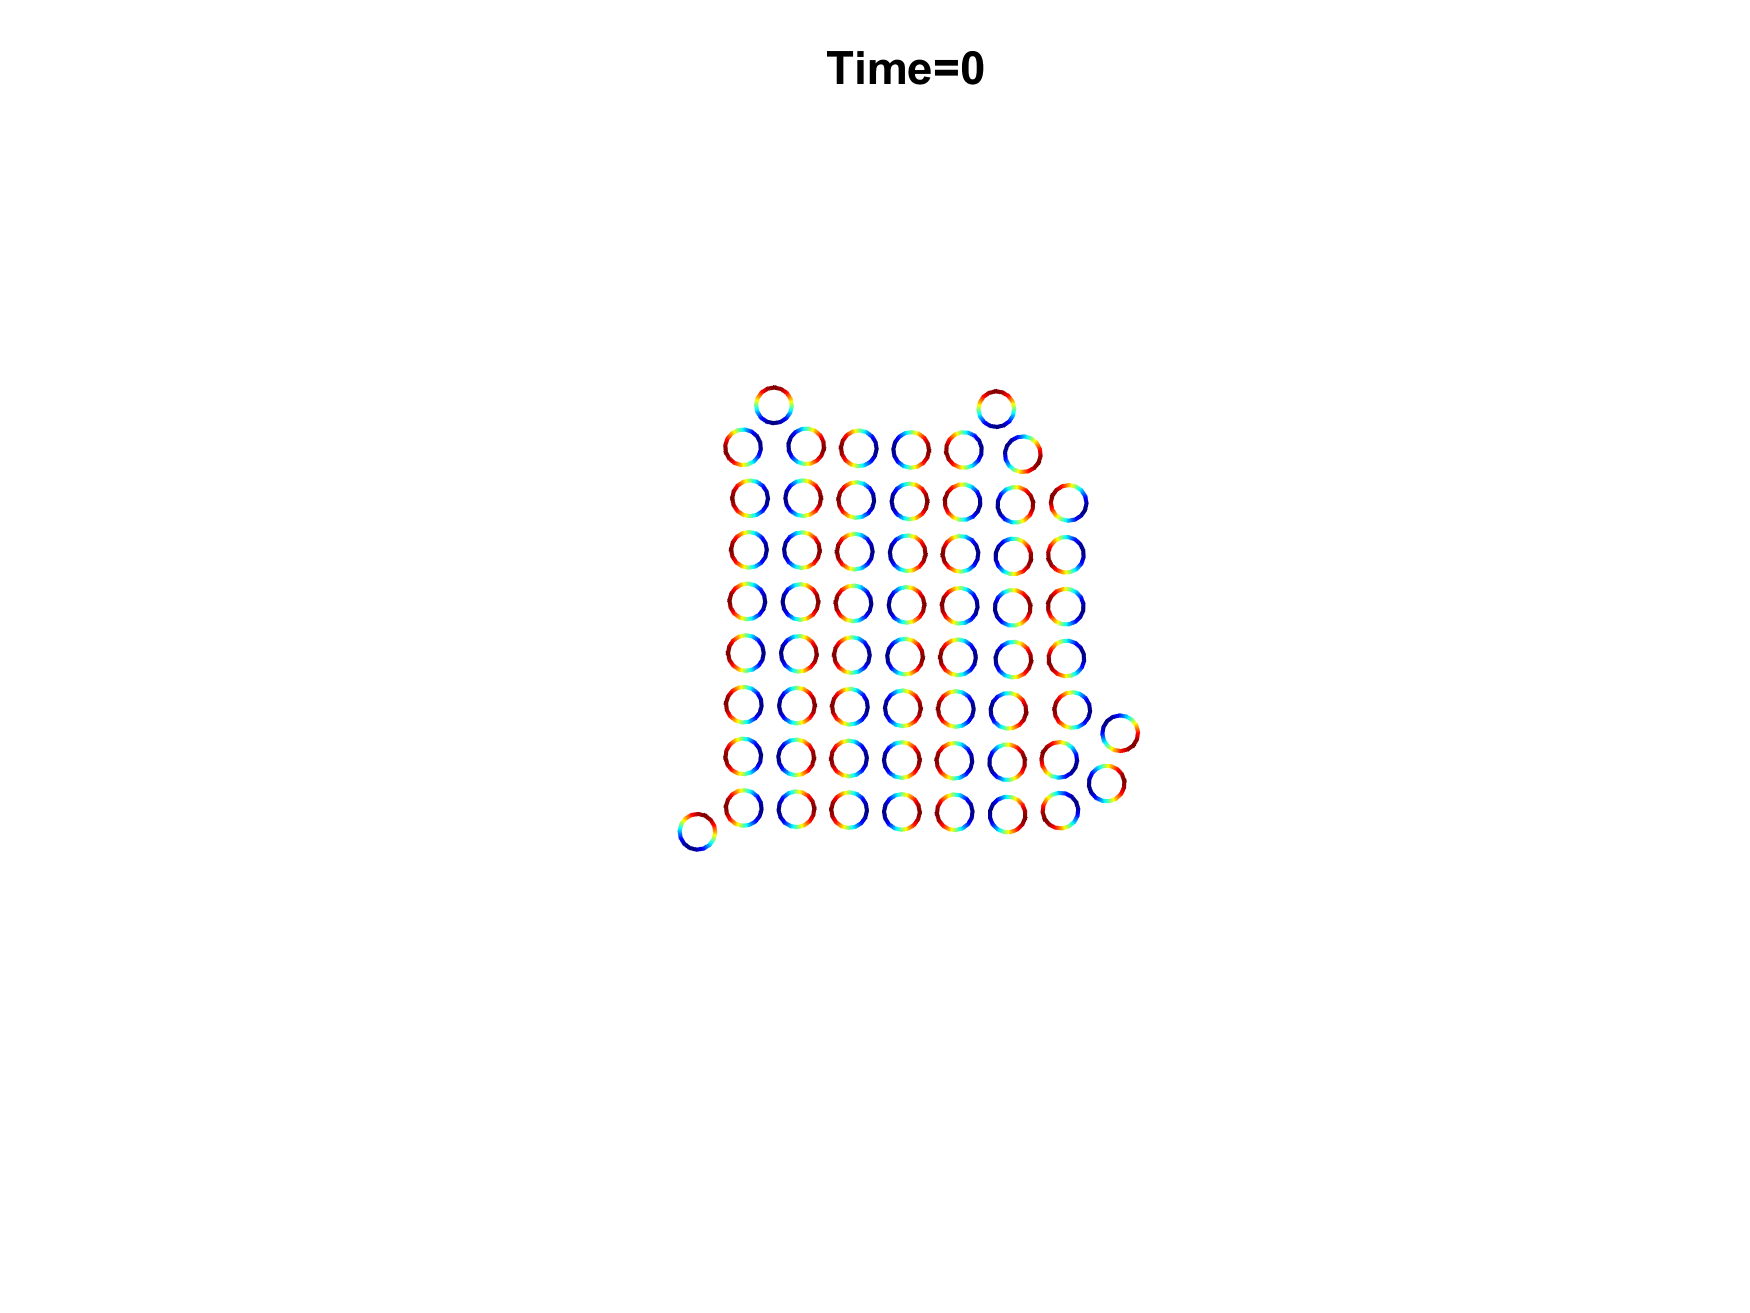
\includegraphics[width=0.21\textwidth]{shear_checker_0.png}
  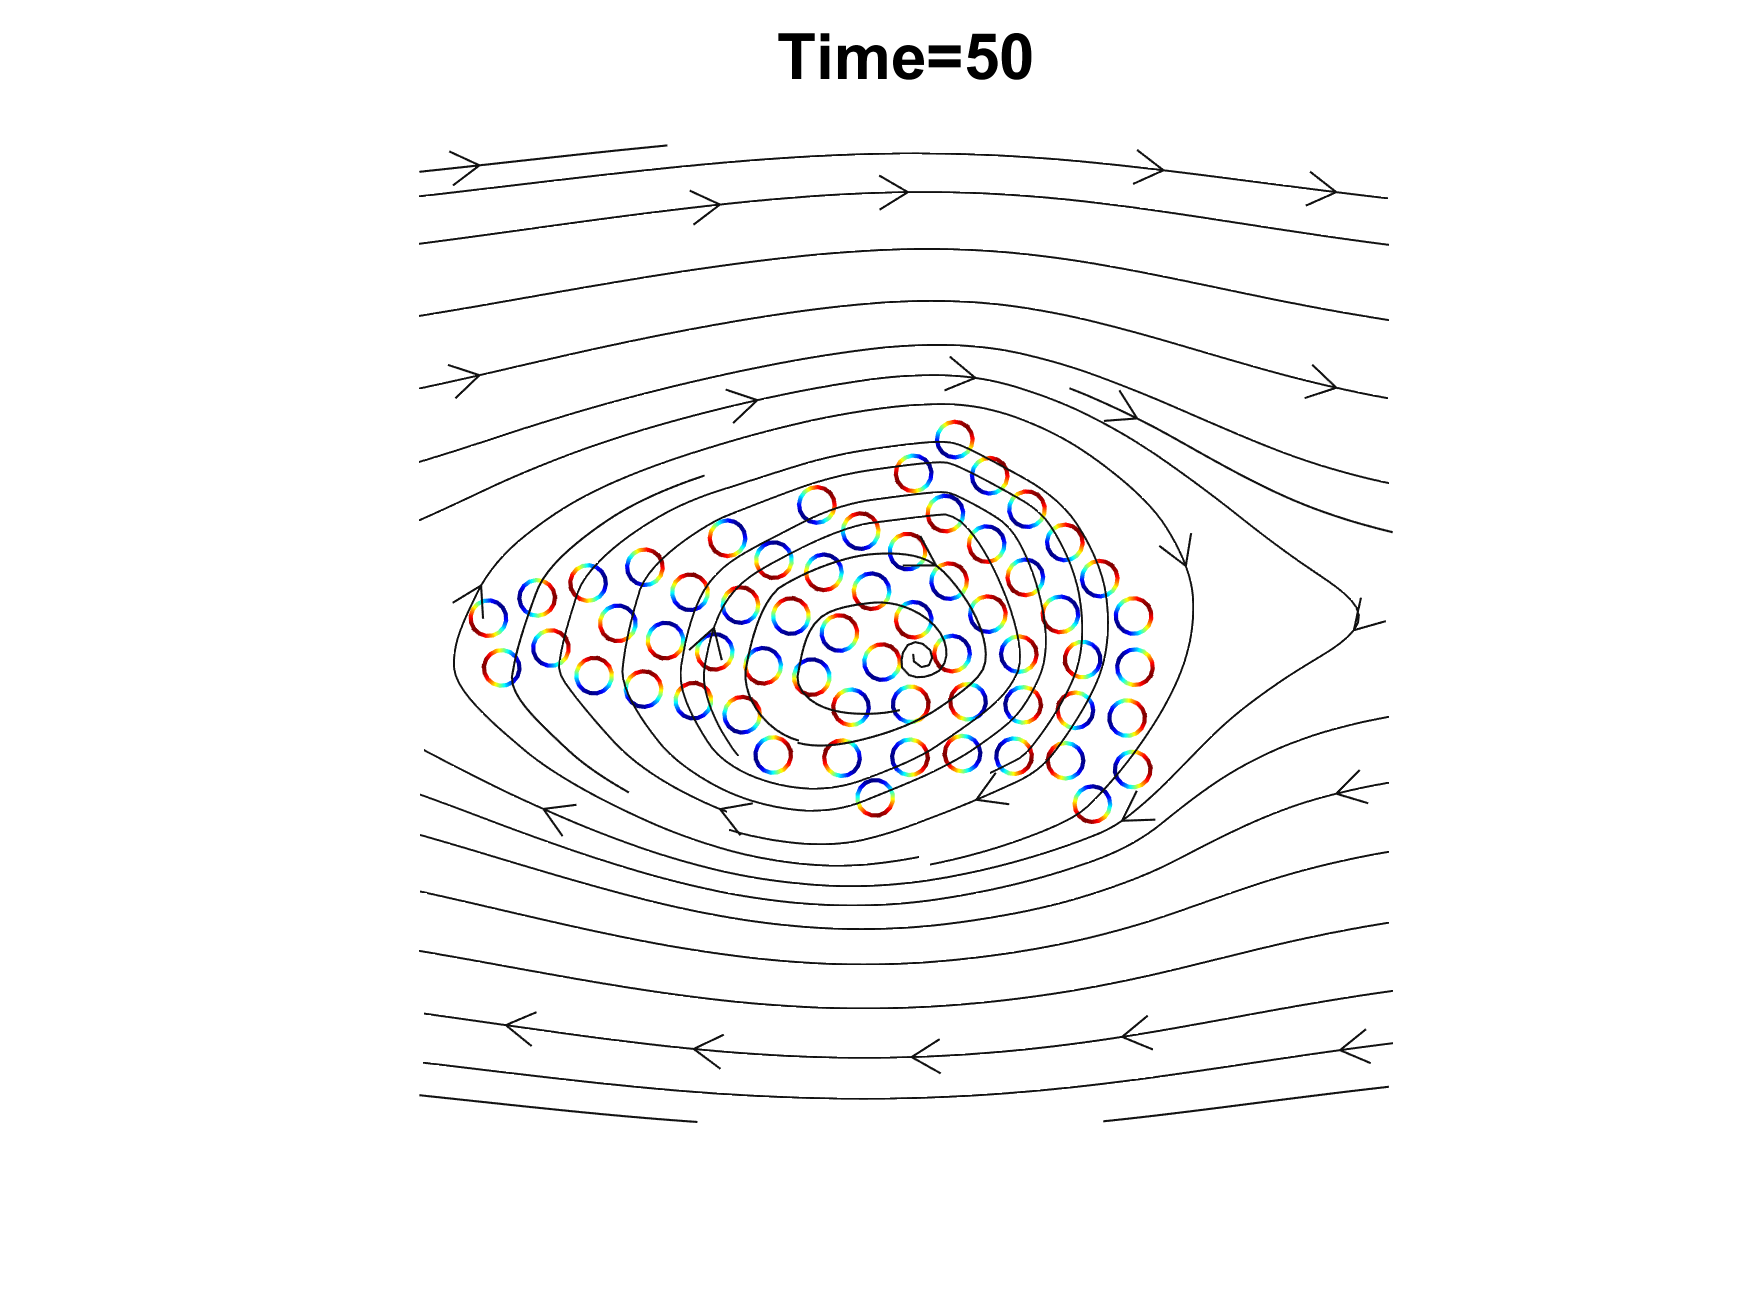
\includegraphics[width=0.21\textwidth]{shear_checker_250.png}
  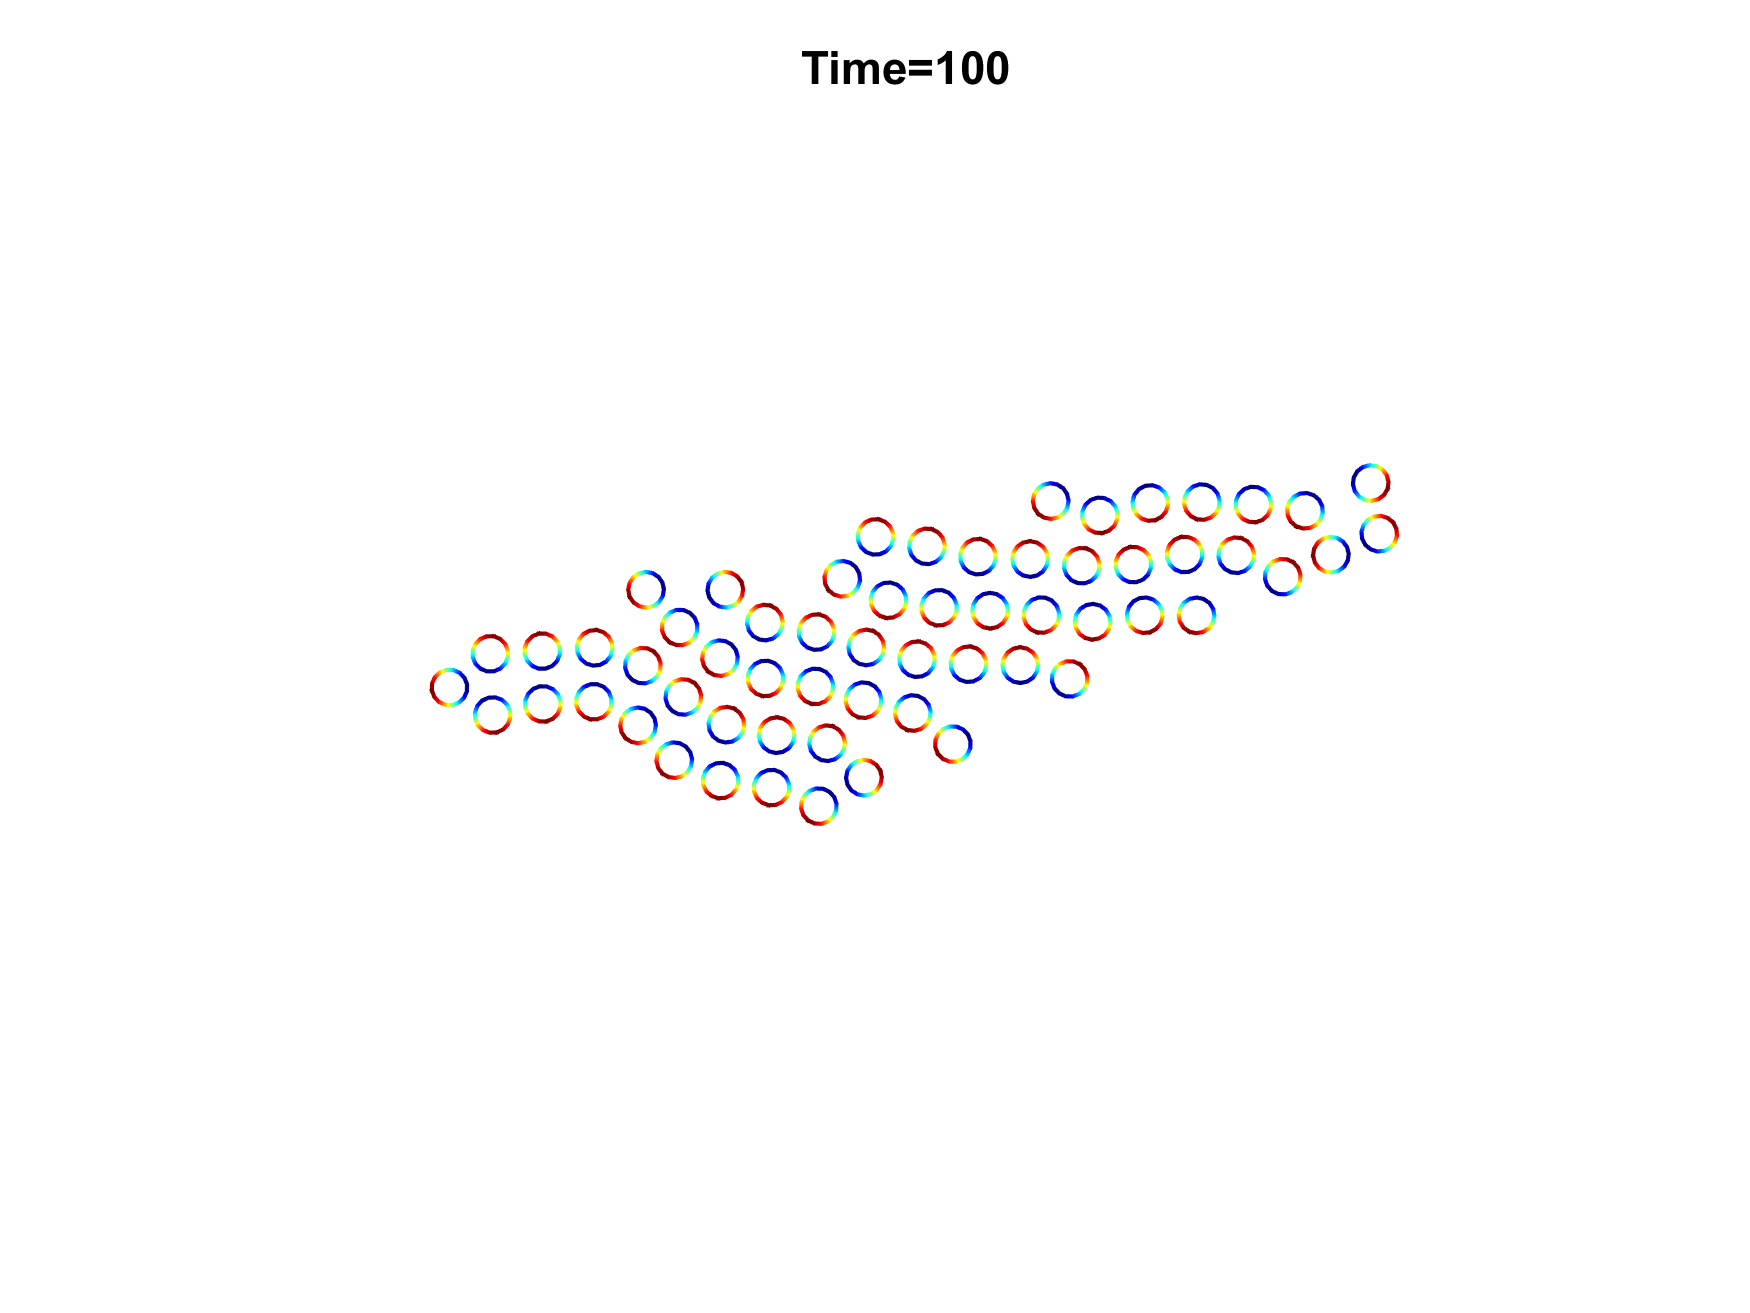
\includegraphics[width=0.21\textwidth]{shear_checker_500.png}
  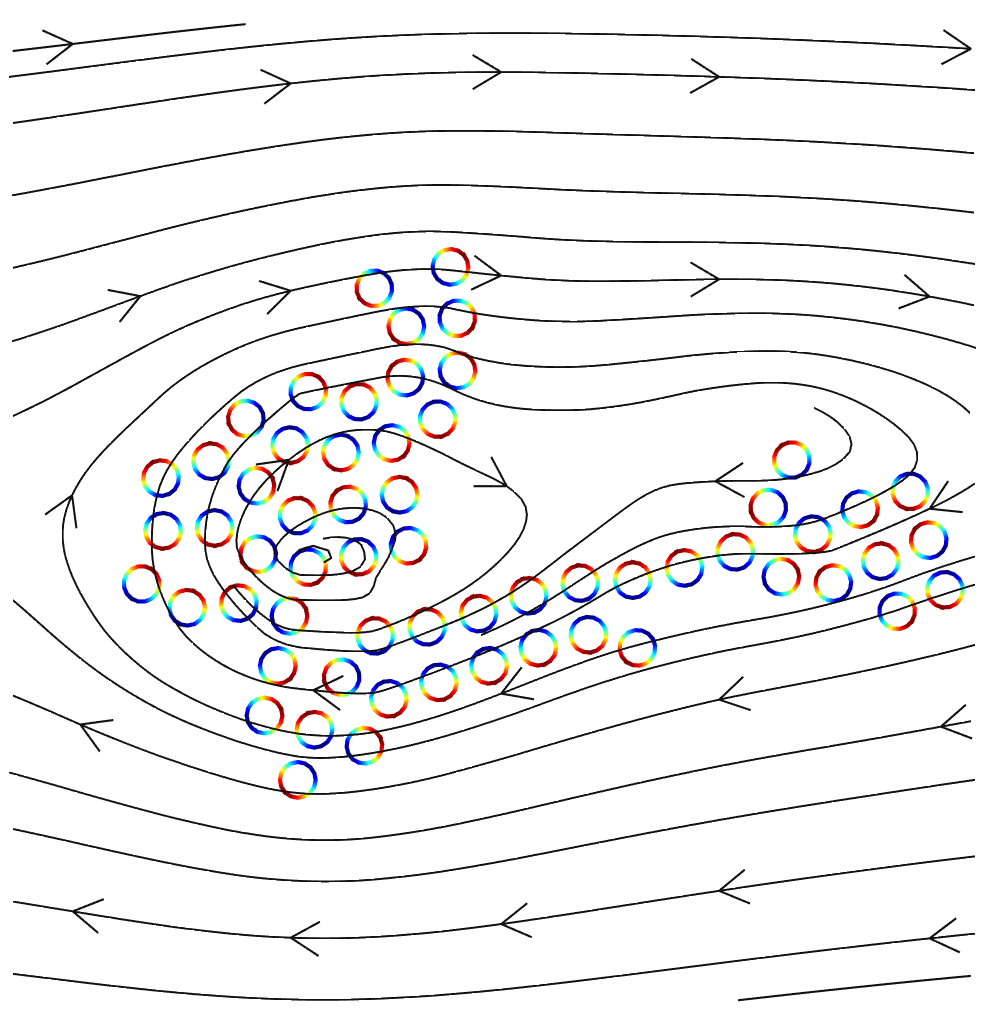
\includegraphics[width=0.21\textwidth]{shear_checker_750.png} \\
  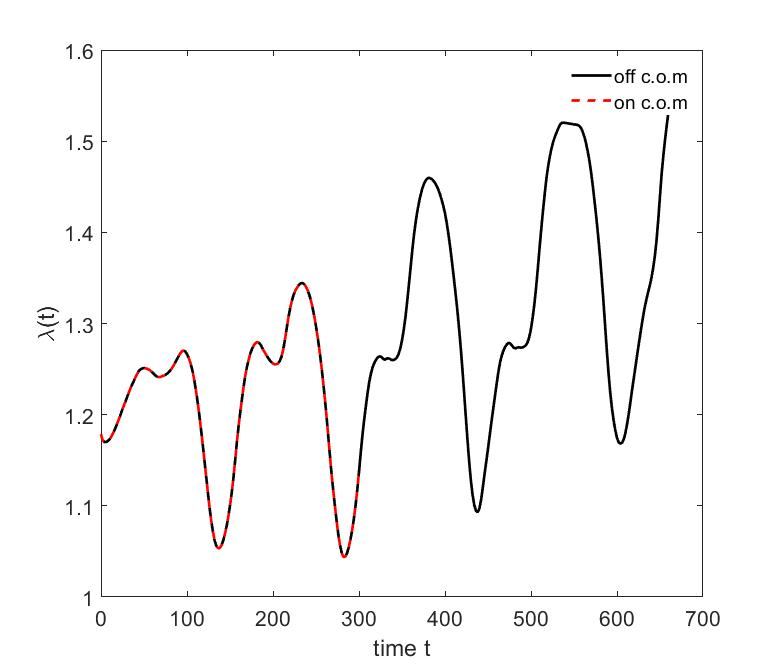
\includegraphics[width=0.4\textwidth]{lambda_fig1.jpg}
  \end{center}
  \vspace{-20pt}  
  \caption{\label{fig:shear_1} Snapshots of simulation using boundary condition \eqref{eq:bcs}(ii) in a shear flow when $\dot\gamma=0.05$. }
\end{figure}
%

%Consider the energy profiles for two simulations where the centor of mass is on and off the origin.
%Fig~\ref{fig:shear_energy1} shows numerical results for both energy profiles and magnitude of energy differences is significantly large when there is a large deformation, for instance, the case when a multi-lamellar structure deformed to a pancake shape.
%
%\begin{figure}
%  \begin{center}
%  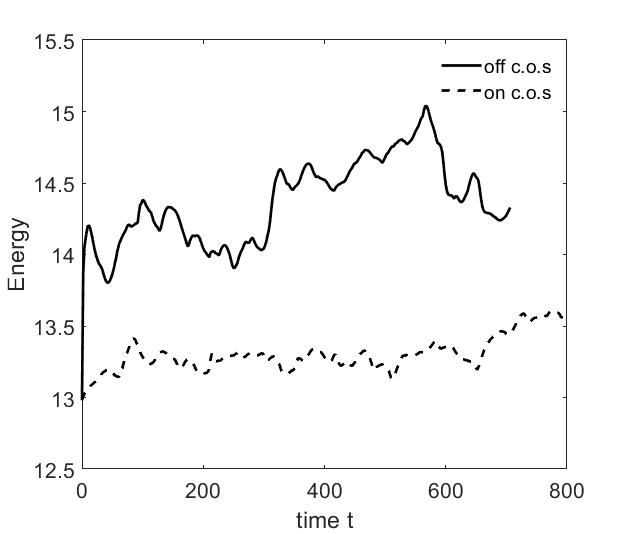
\includegraphics[width=0.5\textwidth]{shear_energy1.jpg}
%  \end{center}
%  \vspace{-20pt}  
%  \caption{\label{fig:shear_energy1} Energy profiles tracked during the simulations using boundary condition \eqref{eq:bcs}(ii) in a shear flow when $\dot\gamma=0.05$. }
%\end{figure}




%%%

The second set of simulation is putting the equilibrium state of the
boundary condition \eqref{eq:bcs} (iii), the checker board, in a shear
flow. After a set of empirical numerical investigations, we obtain a
critical shear rate $\dot\gamma=0.15$ where the checker board deforms
into stripes and small groups of JP. Figure~\ref{fig:shear_2}(a)--(d) show configurations when $t=\{0,50,100,150\}$. %The deformation starts with stripe separations
%
%\begin{figure}
%  \begin{center}
%  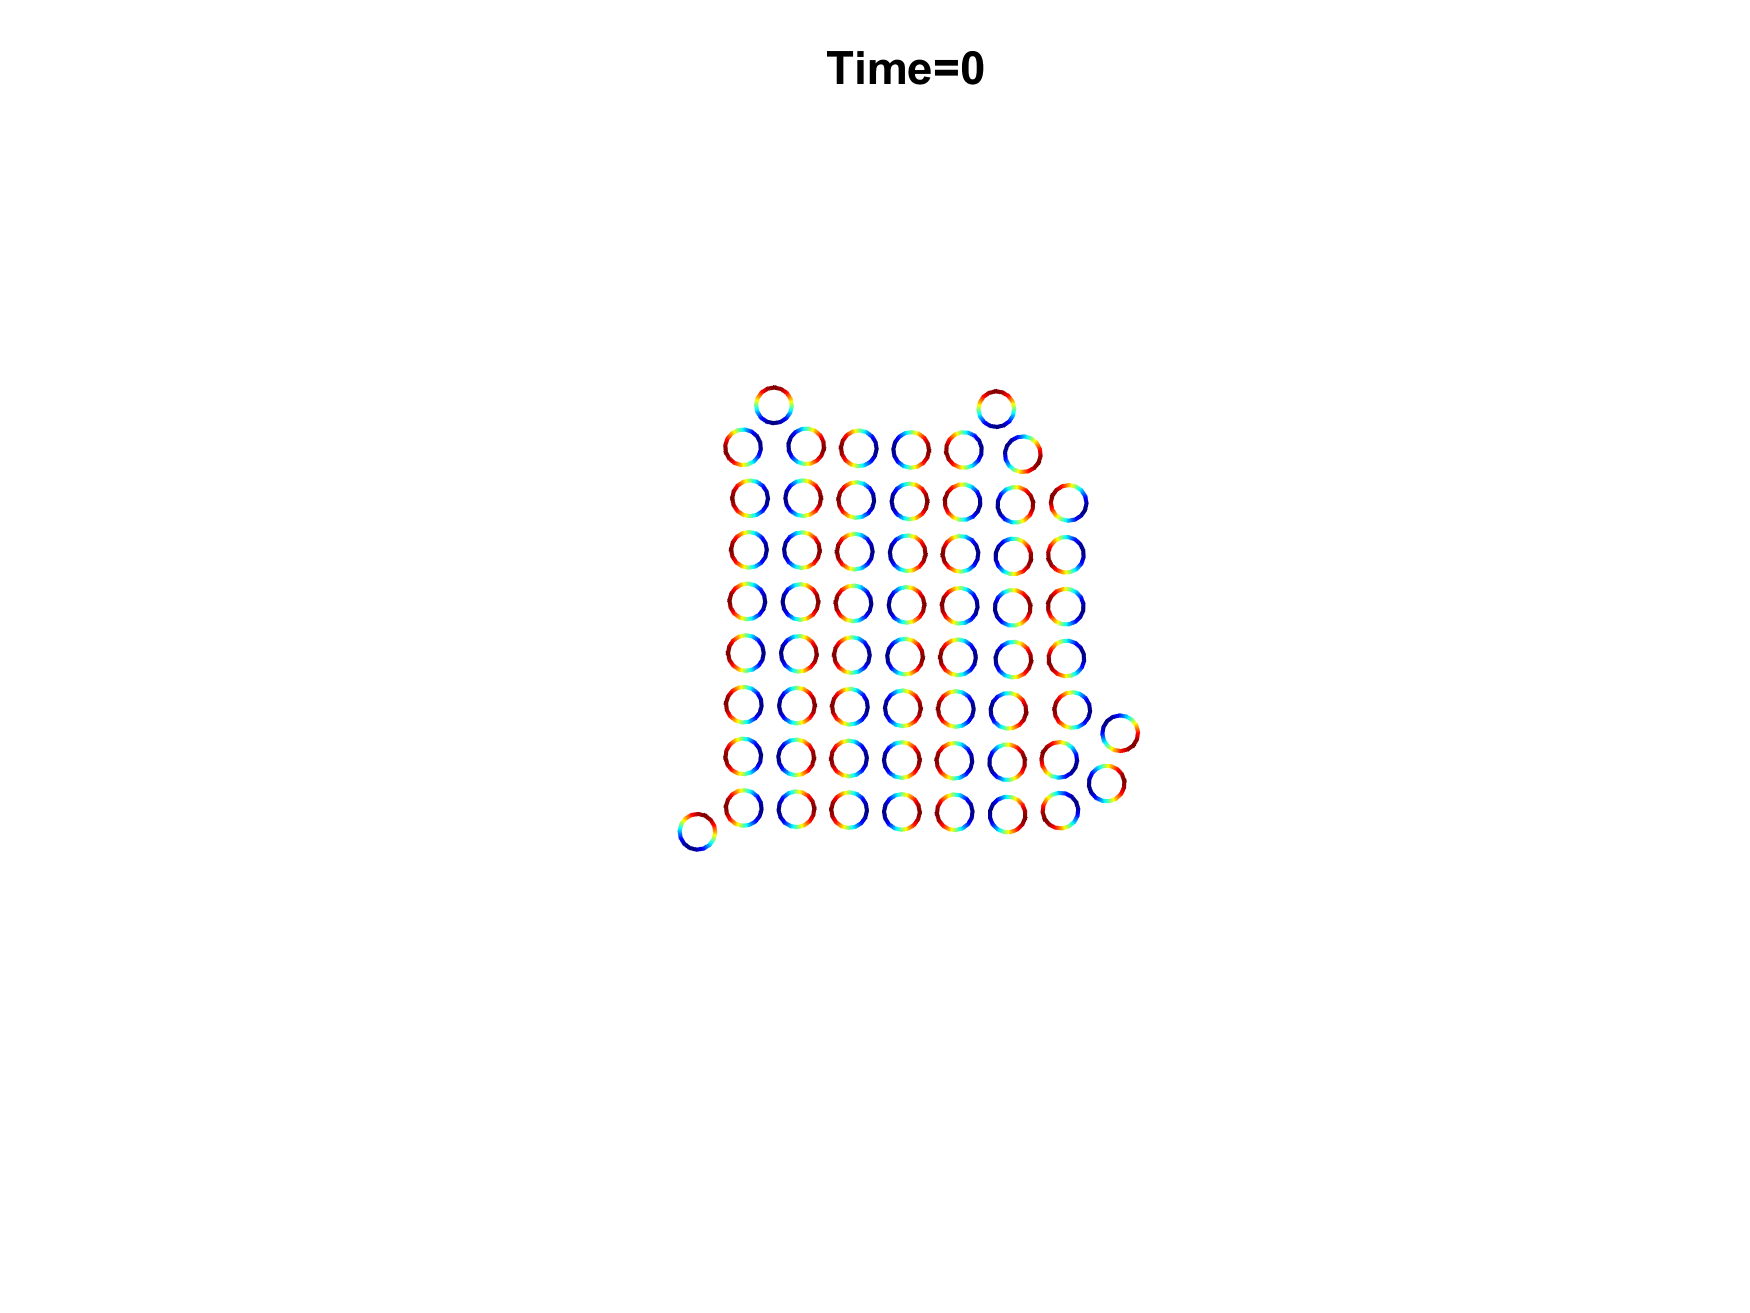
\includegraphics[width=0.4\textwidth]{shear_checker_0.png}
%  \includegraphics[width=0.4\textwidth]{shear_checker_250.png}\\
%  \includegraphics[width=0.4\textwidth]{shear_checker_500.png}
%    \includegraphics[width=0.4\textwidth]{shear_checker_750.png}
%  \end{center}
%  \vspace{-20pt}  
%  \caption{\label{fig:shear_2} Snapshots of simulation using boundary condition \eqref{eq:bcs}(iii) in a shear flow when $\dot\gamma=0.15$. }
%\end{figure}


\subsection{Collective Janus Particles Suspended in a Taylor-Green Flow}

Similar to shear flow simulations, we then place equilibrium states of all boundary conditions \eqref{eq:bcs} in a rotating Taylor-Green Flow with a length scale $l$,
\begin{equation}
\uu_\infty(\xx) = V_0 \left(-\cos(l{\bf e}_x\cdot\xx)\sin(l{\bf e}_y\cdot\xx){\bf e}_x+\sin(l{\bf e}_x\cdot\xx)\cos(l{\bf e}_y\cdot\xx){\bf e}_y\right).
\end{equation}
%
The magnitude of the vortex flow is controlled by the velocity scale
$V_0$.  Similar to the setup in the shear flow cases, we shift the
center of mass position to the origin then turn on the Taylor-Green flow
with $V_0=0.1$ and tune the sides of zero-velocity box to $\pi$, i.e.,
$l=0.5$, Figure~\ref{fig:TG_1}(a)--(c) show three frames of simulation
results and we track the aspect ratio $\lambda$ described in the
previous section which is provided in panel (d).  The stiffness of the
multi-lamellar structure is able to compete with the flow therefore the
structure does not deform to any states other than multi-lamellar shape.
We also found that the flow strength coefficient above $V_0=0.1$ will
result to clear group separations during the simulations.  Comparing
with the case when $V_0=0.2$, we provide a frame in
Figure~\ref{fig:TG_2}(a) and the energy comparison is shown in panel
(b). Numerical results validate the phenomenon that a higher
Taylor-Green vortex flow generates large structure separations with
higher total energy.


\begin{figure}
  \begin{center}
  \includegraphics[width=0.4\textwidth]{TG_0.png}
  \includegraphics[width=0.4\textwidth]{TG_2500.png}\\
  \includegraphics[width=0.4\textwidth]{TG_5000.png}
    \includegraphics[width=0.4\textwidth]{TG_dist.jpg}
  \end{center}
  \vspace{-20pt}  
  \caption{\label{fig:TG_1} Snapshots of simulation using boundary condition \eqref{eq:bcs}(b) in a Taylor-Green flow when $V_0=0.1$ and $l=0.5$.}
\end{figure}


\begin{figure}
  \begin{center}
  \includegraphics[width=0.4\textwidth]{TG0p2_2000.png}
  \includegraphics[width=0.4\textwidth]{TG_energy1.jpg}
  \end{center}
  \vspace{-20pt}  
  \caption{\label{fig:TG_2} (a) Snapshots of simulation using boundary condition \eqref{eq:bcs}(b) in a Taylor-Green flow when $V_0=0.2$, $l=0.5$, and $t = 400$. (b) Energy profiles for two cases $V_0=0.1$ and $V_0=0.2$. }
\end{figure}



\subsection{Steady-State Structure Confined in Narrow Channels}


Here are demonstrations of having JP vesicle and multi-lamellar
structure in a narrow channel under a shear flow.  Simulation results
and snapshots are shown in Figures~\ref{fig:confined_vesicle} and
Figure~\ref{fig:confined_lamellar} where the JP vesicle has $N_b=25$
particles and JP lamellar has $N_b=40$ particles, respectively. Both
starting configurations are pre-relaxed and the channel width in the
narrow part is about 5 length units in the vesicle case and 4 length
units in the lamellar case.


\begin{figure}
  \begin{center}
  \includegraphics[width=0.4\textwidth]{VesConf_0.png}
  \includegraphics[width=0.4\textwidth]{VesConf_2000.png}\\
  \includegraphics[width=0.4\textwidth]{VesConf_5000.png}
  \includegraphics[width=0.4\textwidth]{VesConf_10000.png}
  \end{center}
  \vspace{-20pt}  
  \caption{\label{fig:confined_vesicle} A JP vesicle confined in a narrow channel where $N_b=25$ and $\dot\gamma=0.01$.  }
\end{figure}




\begin{figure}
  \begin{center}
  \includegraphics[width=0.4\textwidth]{MultConf_100.png}
  \includegraphics[width=0.4\textwidth]{MultConf_600.png}\\
  \includegraphics[width=0.4\textwidth]{MultConf_1200.png}
  \includegraphics[width=0.4\textwidth]{MultConf_2400.png}
  \end{center}
  \vspace{-20pt}  
  \caption{\label{fig:confined_lamellar} A JP multi-lamellar structure confined in a narrow channel where $N_b=40$ and $\dot\gamma=0.05$.  }
\end{figure}


\section{Conclusions}




%%%

% If in two-column mode, this environment will change to single-column
% format so that long equations can be displayed. Use
% sparingly.
%\begin{widetext}
% put long equation here
%\end{widetext}

% figures should be put into the text as floats.
% Use the graphics or graphicx packages (distributed with LaTeX2e)
% and the \includegraphics macro defined in those packages.
% See the LaTeX Graphics Companion by Michel Goosens, Sebastian Rahtz,
% and Frank Mittelbach for instance.
%
% Here is an example of the general form of a figure:
% Fill in the caption in the braces of the \caption{} command. Put the label
% that you will use with \ref{} command in the braces of the \label{} command.
% Use the figure* environment if the figure should span across the
% entire page. There is no need to do explicit centering.

% \begin{figure}
% \includegraphics{}%
% \caption{\label{}}
% \end{figure}

% Surround figure environment with turnpage environment for landscape
% figure
% \begin{turnpage}
% \begin{figure}
% \includegraphics{}%
% \caption{\label{}}
% \end{figure}
% \end{turnpage}

% tables should appear as floats within the text
%
% Here is an example of the general form of a table:
% Fill in the caption in the braces of the \caption{} command. Put the label
% that you will use with \ref{} command in the braces of the \label{} command.
% Insert the column specifiers (l, r, c, d, etc.) in the empty braces of the
% \begin{tabular}{} command.
% The ruledtabular enviroment adds doubled rules to table and sets a
% reasonable default table settings.
% Use the table* environment to get a full-width table in two-column
% Add \usepackage{longtable} and the longtable (or longtable*}
% environment for nicely formatted long tables. Or use the the [H]
% placement option to break a long table (with less control than 
% in longtable).
% \begin{table}%[H] add [H] placement to break table across pages
% \caption{\label{}}
% \begin{ruledtabular}
% \begin{tabular}{}
% Lines of table here ending with \\
% \end{tabular}
% \end{ruledtabular}
% \end{table}

% Surround table environment with turnpage environment for landscape
% table
% \begin{turnpage}
% \begin{table}
% \caption{\label{}}
% \begin{ruledtabular}
% \begin{tabular}{}
% \end{tabular}
% \end{ruledtabular}
% \end{table}
% \end{turnpage}

% Specify following sections are appendices. Use \appendix* if there
% only one appendix.
%\appendix
%\section{}



